\documentclass[12pt, oneside]{article}   	% use "amsart" instead of "article" for AMSLaTeX format
\usepackage{geometry}                		% See geometry.pdf to learn the layout options. There are lots.
\geometry{letterpaper}                   		% ... or a4paper or a5paper or ... 
%\geometry{landscape}                		% Activate for for rotated page geometry
%\usepackage[parfill]{parskip}    		% Activate to begin paragraphs with an empty line rather than an indent
\usepackage{graphicx}				% Use pdf, png, jpg, or eps� with pdflatex; use eps in DVI mode
\usepackage{amsmath}
\usepackage{mathtools}
								% TeX will automatically convert eps --> pdf in pdflatex		
\usepackage{amssymb}
\numberwithin{equation}{section}
\numberwithin{table}{section}
\usepackage{color}
\usepackage[toc,page]{appendix}
\usepackage[hypcap]{caption}
\usepackage{caption}
\usepackage{glossaries}
\usepackage{commath}
\usepackage{float}
\usepackage{pbox}
\usepackage{lipsum}
%\usepackage{caption}
\usepackage{subcaption}
\usepackage{wrapfig}
%\usepackage{natbib}
%==== TITLE PAGE ======================================================================================




% Set Margin Sizes
%%%%%%%%%%%%%%%%%%%%%%%%%%%
 \geometry{
 a4paper,
 left= 30mm,
 right= 30mm,
 top= 25mm,
 bottom= 25mm,
 }
%%%%%%%%%%%%%%%%%%%%%%%%%%%
  
% Set Line Spacing
%%%%%%%%%%%%%%%%%%%%%%%%%%%
\usepackage{setspace}
\singlespacing
%\onehalfspacing
%\doublespacing
%\setstretch{1.1}
%%%%%%%%%%%%%%%%%%%%%%%%%%%

\title{\textbf{{Monocular Vision Based SLAM} Using Kinematic State Estimation}\\\vspace{7.5 mm}\Large{by}\\\vspace{7.5 mm}\Large{Aidan Russel Landsberg}\\\vspace{45 mm}\large{Report submitted in partial fulfilment of the requirements of the module Project(E) 448 for the degree Baccalaureus in Engineering in the Department of Electrical and Electronic Engineering at the University of Stellenbosch}\\\vspace{45mm}\large{Department of Electrical and Electronic Engineering,\\ University of Stellenbosch,\\
Private Bag X1, Matieland 7602, South Africa.}\\\vspace{20mm}\large{Supervisor: Dr. C.E. (Corn\'{e}) Van Daalen}}
\date{May 2015}	% Activate to display a given date or no date
						
\usepackage{eso-pic}
\newcommand\BackgroundPic{
\put(0,0){
\parbox[b][\paperheight]{\paperwidth}{%
\vfill
\centering

\includegraphics[keepaspectratio]{Figures/crest.JPG}%
\vfill
}}}

\begin{document}

\AddToShipoutPicture*{\BackgroundPic}

\maketitle
\thispagestyle{empty}
\newpage
\thispagestyle{empty}
%%%%%%%%%%%%%%%%%%%%%%%%%%%%%%%%%%%%%%%%%%%%%%%%%%%%%%%%%%%%%%%%%%%%%%%%%%
 \newgeometry{
 a4paper,
 left= 30mm,
 right= 20mm,
 top= 25mm,
 bottom= 25mm,
 }
%%%%%%%%%%%%%%%%%%%%%%%%%%%%%%%%%%%%%%%%%%%%%%%%%%%%%%%%%%%%%%%%%%%%%%%%%%
\newpage
\section*{Summary}
This study seeks to improve localisation using a single camera as the measurement sensor. Simultaneous localisation and mapping  (SLAM) is implemented using a kinematic state estimator. In this implementation, an inertial measurement unit measures the movement of the system and the kinematic state estimator aims to accurately predict this trajectory while the camera images are used to potentially correct errors made in the prediction.The theory necessary to derive the system from first principles is discussed before this theory is used to implement the design of the system. The results of this system show that the kinematic state estimator works correctly although a full implementation is not possible yet. 
\thispagestyle{empty}
%%%%%%%%%%%%%%%%%%%%%%%%%%%%%%%%%%%%%%%%%%%%%%%%%%%%%%%%%%%%%%%%%%%%%%%%%%
\newpage
\section*{Opsomming}
Hierdie artikel poog om die lokalisering van 'n robot te verbeter met meetings van 'n enkele kamara. Gelyktydige plek en kaarting (SLAM) word gebruik deur die hulp van 'n kinematiese afstaker. In hierdie implementering, 'n traagheid meeteenheid word gebruik om die dynamika van die stelsel te meet.  Die theorie agtergrond nodig om so 'n implementering van SLAM te inkorporeer word bespreek. Die afleiding nodig om die ontwerp te realieseer word ook bespreek. Die resultaten van die stelsel wis dat die kinematiese afstaken wel koek werk alhoewel die stelsel volledig nie geimplementeer word nie.    
\newpage
%%%%%%%%%%%%%%%%%%%%%%%%%%%%%%%%%%%%%%%%%%%%%%%%%%%%%%%%%%%%%%%%%%%%%%%%%%
%%%%%%%%%%%%%%%%%%%%%%%%%%%%%%%%%%%%%%%%%%%%%%%%%%%%%%%%%%%%%%%%%%%%%%%%%%
%%%%%%%%%%%%%%%%%%%%%%%%%%%%%%%%%%%%%%%%%%%%%%%%%%%%%%%%%%%%%%%%%%%%%%%%%%
%%%%%%%%%%%%%%%%%%%%%%%%%%%%%%%%%%%%%%%%%%%%%%%%%%%%%%%%%%%%%%%%%%%%%%%%%%
%%%%%%%%%%%%%%%%%%%%%%%%%%%%%%%%%%%%%%%%%%%%%%%%%%%%%%%%%%%%%%%%%%%%%%%%%%
% Report Begins
%%%%%%%%%%%%%%%%%%%%%%%%%%%%%%%%%%%%%%%%%%%%%%%%%%%%%%%%%%%%%%%%%%%%%%%%%%
%%%%%%%%%%%%%%%%%%%%%%%%%%%%%%%%%%%%%%%%%%%%%%%%%%%%%%%%%%%%%%%%%%%%%%%%%%
%%%%%%%%%%%%%%%%%%%%%%%%%%%%%%%%%%%%%%%%%%%%%%%%%%%%%%%%%%%%%%%%%%%%%%%%%%
\pagenumbering{roman}
%%%%%%%%%%%%%%%%%%%%%%%%%%%%%%%%%%%%%%%%%%%%%%%%%%%%%%%%%%%%%%%%%%%%%%%%%%
\newpage
\section*{Acknowledgements}
%\addcontentsline{toc}{section}{Acknowledgements}
I would like to express my sincere gratitude toward the following individuals for their role in this project:\\

\begin{itemize}
\item My heavenly Father, for providing me with the intellectual capacity, guidance and support necessary during this project while remaining faithful and true in the toughest of times.\\
\item My study leader, Dr. Corn\'{e} Van Daalen, for his endless enthusiasm, guidance, patience, support, time and invaluable insight. As well as for personally setting aside the time to propose and supervise this project. \\
\item My parents, for their endless support and motivation. As well as for making all the necessary sacrifices to provide me with the opportunity to complete this project. \\
\item Mr. Arno Barnard, for his advice regarding the embedded design.\\
\item My girlfriend Bianca La Gorc\'{e}, for supporting me endlessly.\\
\item Benjamin Pannell, for being a great personal mentor and friend. As well as for providing me with insight regarding various software concepts. \\
\item Luca Duesimi, for aiding in the design and construction of the stability platform. \\
\item Warren Farmer, Kurt Coetzer and Lowku Leeuwenaar, for helping construct the stability platform.       
\end{itemize}
\newpage
%%%%%%%%%%%%%%%%%%%%%%%%%%%%%%%%%%%%%%%%%%%%%%%%%%%%%%%%%%%%%%%%%%%%%%%%%%
\section*{Declaration}
%\addcontentsline{toc}{section}{Declaration}
I, the undersigned, hereby declare that the work contained in this report is my own original work unless indicated otherwise.
\vspace{200mm}
\\
Signature.....................................................		Date..........................................................
\newpage
%%%%%%%%%%%%%%%%%%%%%%%%%%%%%%%%%%%%%%%%%%%%%%%%%%%%%%%%%%%%%%%%%%%%%%%%%%
% Table of contents
%%%%%%%%%%%%%%%%%%%%%%%%%%%%%%%%%%%%%%%%%%%%%%%%%%%%%%%%%%%%%%%%%%%%%%%%%%
%%%%%%%%%%%%%%%%%%%%%%%%%%%%%%%%%%%%%%%%%%%%%%%%%%%%%%%%%%%%%%%%%%%%%%%%%%
\tableofcontents
\newpage

\listoffigures
\listoftables
%%%%%%%%%%%%%%%%%%%%%%%%%%%%%%%%%%%%%%%%%%%%%%%%%%%%%%%%%%%%%%%%%%%%%%%%%%
\newpage
\section*{Acronyms}
%\addcontentsline{toc}{section}{Acronyms}
\begin{table}[h]
\caption*{}
%\begin{center}
\begin{tabular}{l l}
\textbf{2D} 	 & Two-dimensional \\
\textbf{3D} 	 & Three-dimensional \\
\textbf{CMOS}	 & Complementary Metal-Oxide Semiconductor \\   
\textbf{EKF}	 & Extended Kalman Filter \\
\textbf{GPIO}    & General-purpose input/output \\
\textbf{IMU} 	 & Inertial Measurement Unit \\
\textbf{KF}         & Kalman Filter \\
\textbf{I2C}	 & Inter-Integrated Circuit Bus \\
\textbf{ISR}	 & Interrupt Service Routine \\
\textbf{LIDAR}   & Light Detection and Ranging \\
\textbf{MonoSLAM} & Monocular Simultaneous Localisation and Mapping \\
\textbf{PDF}	 & Probability Density Function \\ 
\textbf{PTAM} 	 & Parallel Tracking and Mapping \\ 
\textbf{RV}	 & Random Variable \\
\textbf{SIS} 	 & Sequential Importance Sampling \\
\textbf{SPI} 	 & Serial Peripheral Interface \\
\textbf{SLAM} 	 & Simultaneous Localisation and Mapping \\
\textbf{USB} 	 & Universal Serial Bus
\end{tabular}
%\end{center}
\label{accr}
\end{table}%

\newpage
%%%%%%%%%%%%%%%%%%%%%%%%%%%%%%%%%%%%%%%%%%%%%%%%%%%%%%%%%%%%%%%%%%%%%%%%%%
\section*{List of Symbols}
%\addcontentsline{toc}{section}{List of Symbols}
\begin{table}[h]
\caption*{}
%\begin{center}
\begin{tabular}{l l}
$W$ & Inertial reference fame \\
$C$ & Camera's free coordinate body frame \\
$\Delta T$ & Sampling instance \\
$ \pi $ & Constant denoting the ratio between a circles radius and its circumference \\
$\boldsymbol{\mu}$ & Mean vector of a Gaussian random variable \\
$\boldsymbol{\Sigma}$ & Covariance matrix of a Gaussian random variable \\
$\eta$ & Normalisation contant \\
$ \textbf{I}$ & Identity matrix \\
$\boldsymbol{\omega}$ & angular velocity (expressed in radians per second)\\
$\textbf{R}^{CW}$ & Rotation matrix projecting an entity from the body frame to the inertial frame \\ 
$\textbf{C}$ & Camera calibration matrix\\
$f$ & Focal length of camera\\
$k_u$ & Focal length normalisation constant\\
$k_v$ & Focal length normalisation constant\\
$u_0$ & Principal Point $x$-coordinate \\
$v_0$ & Principal Point $y$-coordinate \\ 
\end{tabular}
%\end{center}
\label{sym}
\end{table}%

\newpage
%%%%%%%%%%%%%%%%%%%%%%%%%%%%%%%%%%%%%%%%%%%%%%%%%%%%%%%%%%%%%%%%%%%%%%%%%%
\section*{Notation}
%\addcontentsline{toc}{section}{Notation}
\begin{table}[h]
\caption*{}
\begin{center}
\begin{tabular}{|c | l|}
\hline
\textbf{Notation} &  \textbf{Entities}\\
\hline
\hline
$x$ 			& Lower case italic text represents a scalar\\
\hline
$x^W$ 		& Superscripts represent the coordinate frame (e.g. $W$ or $C$) \\
\hline
$\textbf{X}^{x}$ 	& Capital boldface text with a superscript variable represents a Jacobian\\
\hline
$x^T$		& Superscript $T$ however represents the transpose \\
\hline
$x_t$ 		& Subscripts bind a values to a specific instance (e.g. time or feature) \\
\hline
$\bar x$		& Overscore text represent an estimate \\
\hline
$\abs x$		& A modulus denotes the absolute value \\ 
\hline
$\norm x$		& A double modulus denotes the norm \\ 
\hline
$\dot{x}$		& Dot symbols represent derivatives\\
\hline
$\textbf{x}$ 	& Lowercase boldface text represents a vector \\ 
\hline
\textbf{X}		& Capital boldface text represents a Matrix \\
\hline
\hline
			& \textbf{Processes} \\
\hline
\hline
$quat(x)$		& Function that converts a variable into a quaternion  \\
\hline
$bel(x)$ 		& Function that computes the Belief \\
\hline
$x\otimes x$ 	& Represents a quaternion multiplication\\
\hline
$\cfrac{d x}{d t}$ & Liebniz's notation to denote a standard derivative \\		
\hline
$\cfrac{\partial x}{\partial t}$ & Liebniz's notation to denote a partial derivative \\		
\hline
\end{tabular}
\end{center}
\label{not}
\end{table}%
\newpage
%%%%%%%%%%%%%%%%%%%%%%%%%%%%%%%%%%%%%%%%%%%%%%%%%%%%%%%%%%%%%%%%%%%%%%%%%%

%%%%%%%%%%%%%%%%%%%%%%%%%%%%%%%%%%%%%%%%%%%%%%%%%%%%%%%%%%%%%%%%%%%%%%%%%%
\newpage
% Introduction
\pagenumbering{arabic}
%%%%%%%%%%%%%%%%%%%%%%%%%%%%%%%%%%%%%%%%%%%%%%%%%%%%%%%%%%%%%%%%%%%%%%%%%%
\section{Introduction}
%%%%%%%%%%%%%%%%%%%%%%%%%%%%%%%%%%%%%%%%%%%%%%%%%%%%%%%%%%%%%%%%%%%%%%%%%%
\subsection{Robotic Localisation and Mapping}
\textit{Robotics} aims to equip machines with the capability of operating autonomously in the physical world to serve various practical purposes. These machines (robots) are designed to resemble human behaviour and action, so that they can substitute for humans in unknown and potentially hazardous environments ranging from planetary exploration to assembly lines~\cite{mars,indus}. To achieve complete autonomous operation, it is essential that the robot is capable of observing its surrounding environment, subsequently building a map thereof in order to locate itself within this map. The aforementioned processes are more commonly referred to as \textit{map building} and \textit{localisation} respectively. Ultimately, the physical world presents many unforeseen factors and circumstances. These factors contribute to \textit{uncertainty} and generally emerge due to a robot's lack of critical information. Factors such as environments, sensors, robots, models and computation all lead to an increase in uncertainty and can prohibit accurate map building and subsequently, localisation. \textit{Probabilistic robotics} however, models these uncertainties mathematically in order to provide fundamental probabilistic algorithms that can be used to obtain reasonably accurate and efficient solutions to map building and localisation. 

\textit{Occupancy grid mapping} is map building algorithm that uses probabilistic algorithms. Initially presented in a study by Elfes and Moravec~\cite{occupancy}, occupancy grid mapping seeks to calculate the probability that a given position in the environment is occupied by an obstacle. Occupancy grid mapping typically uses range sensors, such as sonar or laser range finders to calculate these probabilities and represent them in a \textit{dense} spatial map. An example of an occupancy grid map is depicted in Figure~\ref{fig:occgrid}. The disadvantages of using occupancy grid mapping however, is that the robot's pose (a robot's position and orientation) is assumed to be known and that the environment is assumed to be static, limiting the practical applications thereof. A further overview of alternative map generating techniques is presented in a study by Thrun~\cite{thrun2007}.     
\begin{figure}[H]
\centering%\begin{center}
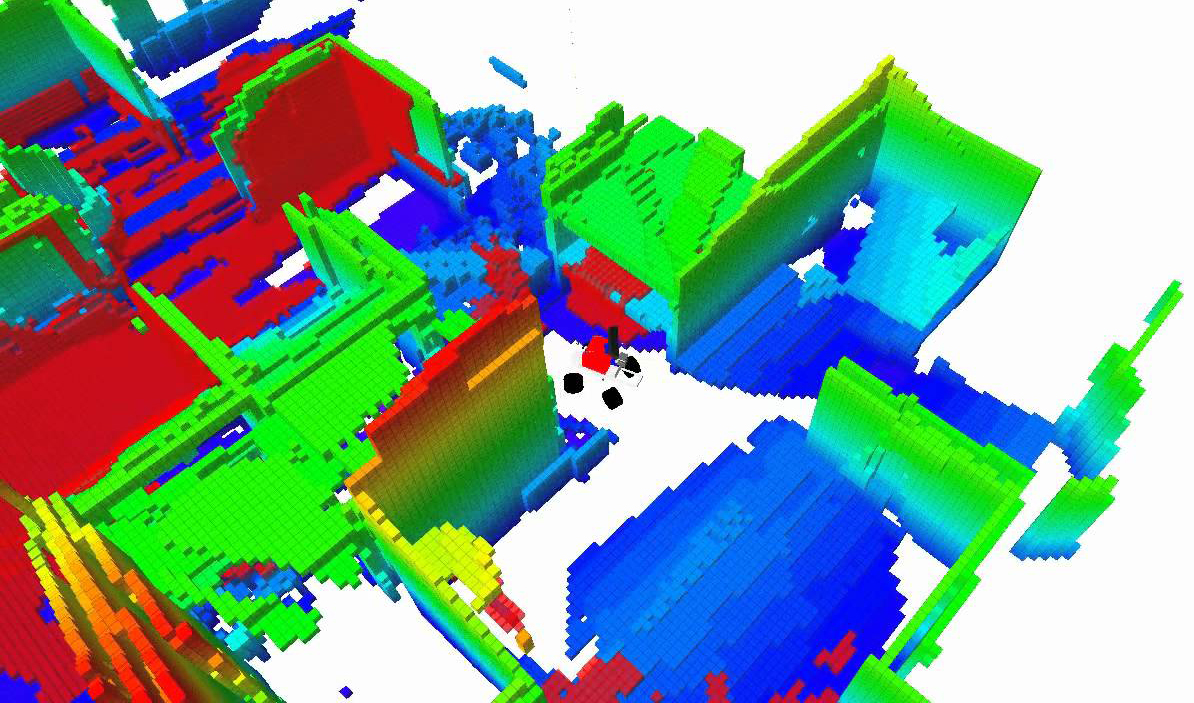
\includegraphics[width=0.49\textwidth, height=0.3\textwidth]{Figures/grid1.jpg}
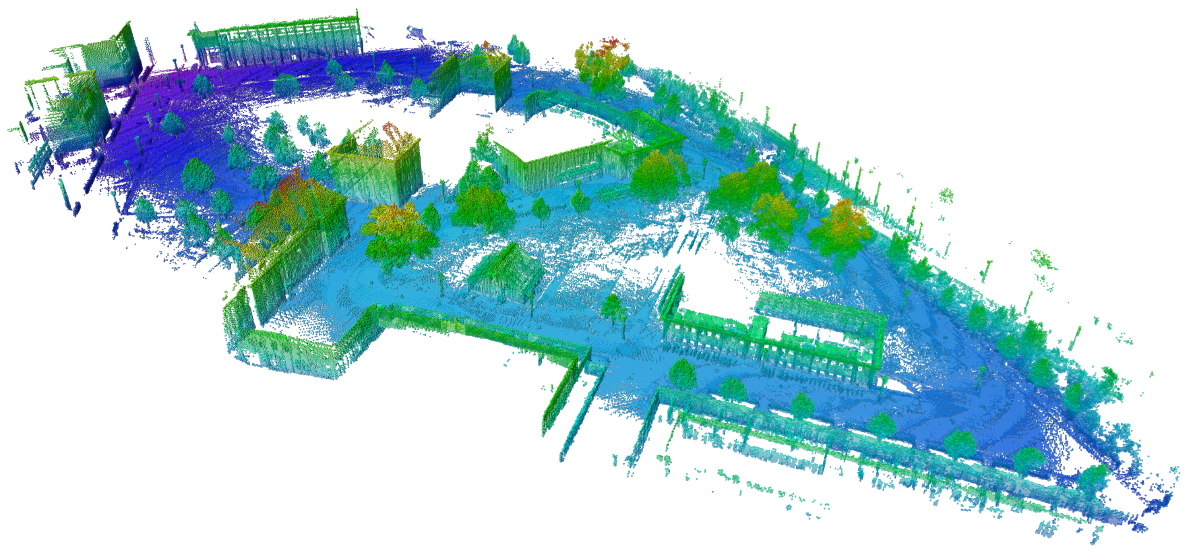
\includegraphics[width=0.49\textwidth, height=0.3\textwidth]{Figures/occ2.png}
\caption{Examples of three-dimensional (3D) occupancy grid (dense) maps. Adapted from~\cite{octomap}.}
\label{fig:occgrid}
%\end{center}
\end{figure} 
Solutions to the \textit{Simultaneous localisation and mapping} (SLAM) problem however, presents methods that concurrently realises map building and localisation~\cite{slam}. SLAM can be described as utilising both the sensor measurements and the control inputs of the robot to construct a continuously expanding map of features in the surrounding environment, while concurrently estimating its location with respect to these features. The sensor measurements provide information about the robot's surroundings and the control inputs provide the information about how the robot is moving. A SLAM map typically represents the locations of its features as a \textit{sparse} set (as opposed to a dense occupancy grid map). An example of a SLAM map is depicted in Figure~\ref{fig:map}. 

The relationship between map building and localisation remains essential to the SLAM problem. If the localisation technique is incorrect, subsequently obtained sensor information will be incorrect, resulting in map estimates that differ from the actual state of the environment. An incorrectly modelled environment will render the sensor information useless, as this information will not correspond with those expected by the constructed map. Ultimately, the resulting localisation approximation will drift over time and eventually become extremely inaccurate. Most modern realisations of SLAM rely on certain probabilistic methods, namely \textit{recursive state estimation} to provide suitable estimates that minimise the uncertainty regarding the mapping and localisation relationship. 

The most commonly used recursive state estimation techniques include both~\textit{optimal filtering} techniques~\cite{ekfslam} as well as \textit{sequential importance sampling} (SIS) techniques~\cite{fast,fast2}. The differences regarding the aforementioned methods can be described as follows: an optimal filtering technique only considers a single hypothesis upon modelling, whereas SIS techniques consider multiple hypothesis. A further summary regarding the aforementioned probabilistic approaches is provided in a study by Chen~\cite{chen2003}.

\begin{figure}[H]
\centering
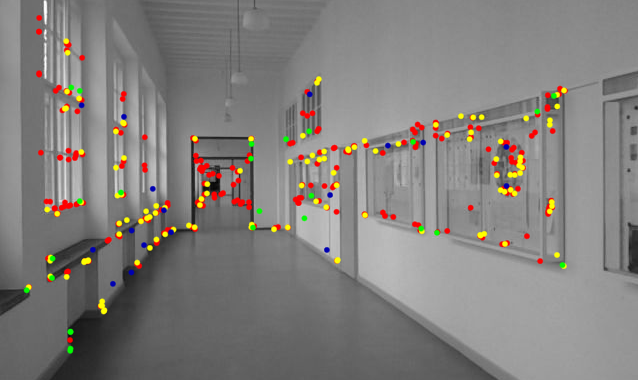
\includegraphics[width=0.49\textwidth, height=0.3\textwidth]{Figures/PTAM_cam.png}
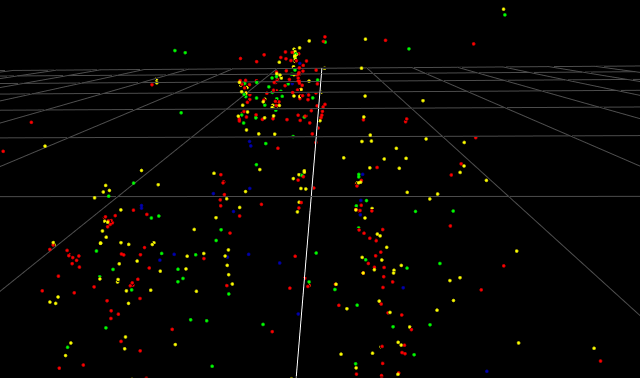
\includegraphics[width=0.49\textwidth, height=0.3\textwidth]{Figures/PTAM_map.png}
\caption{Left: Image frame indicating the feature points. Colours represent the size of a feature (warm colours being the smallest and cool colours being the largest). Right: Reconstructed SLAM three-dimensional (3D) map depicting the feature points with respect to a ground plane (shown as a grid). Adapted from~\cite{scale_visodom}.}
\label{fig:map}
\end{figure}

%Other fundamental parameters and specifications (type of measurement sensor, map dimensionality and sparsity etc.) also determine which specific implementation of the SLAM problem is most applicable. Generally, the main distinguishment between the various realisations of SLAM is the choice of sensor. \\\\
The choice of implementation to solve the SLAM problem will primarily depend on the type of sensor(s) along with the time constraint imposed upon the application (e.g. online map generation vs. offline map generation). Furthermore parameters such as the resultant map's dimensionality as well as their sparsity representation (e.g. point clouds or sparse sets) are typically considered upon a suitable implementation. 

Figure~\ref{fig:slam} depicts the SLAM procedure and is further explained in Table~\ref{tab:Slam}. The robot stores an internal representation (or estimate) of the positions of the features, its pose as well as the uncertainty associated with each of these entities. It should be noted that these uncertainties are not statistically independent of one another. At each frame, a \textit{prediction} regarding the robot's pose, a \textit{measurement} of the observed feature and an \textit{update} of the internal representation is made. 
%\subsubsection{Range Finder Approaches}
%Range finder approaches utilise a beam or a wave to determine the distance to an obstacle in the environment. Generally, the distance to an obstacle from the range finder can be obtained through measuring the time it takes for a pulse generated in a beam/wave to return to the transmitter, after it has reflected off the obstacle. Two-dimensional range finders are only able to obtain these aforementioned distances in a given plane at an opening angle (e.g. range finders with an opening angle of $180^{\circ}$ obtain all range measurements within a $180^{\circ}$ field of view in the given plane). Three-dimensional range finders however, aren't limited to a single plane and can obtain range measurements in all planes within a field of view equivalent to the opening angle. The 3D point in space where the pulse is reflected can then be reconstructed given that the orientation of the range finder are known, resulting in a 3D point cloud. Range finder approaches include sonar, laser, infra-red and ultrasonic. Laser range finders, more commonly referred to as LIDAR (Light Detection And Ranging) are generally considered to provide the best accuracy, especially with regard to depth measurements. The choice of range finder however, varies dependent on the application and specifications of the system at hand.\\
%Range finders obtain large amounts of data regarding the range to obstacles in the environment, especially in the 3D map case. As a result, non-probabilistic methods (as opposed to those previously discussed) are implemented. One such method, namely \textit{scan matching}, aims to merge overlapping point clouds into a single point cloud. This approach, like many range finder approaches however, generally present a great cost in both processing as well as finance. 

\begin{figure}[H]
\centering%\begin{center}
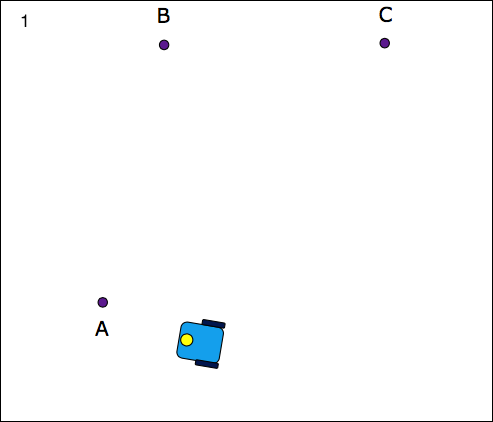
\includegraphics[width=0.32\textwidth, height=0.25\textwidth]{Figures/step1.png}
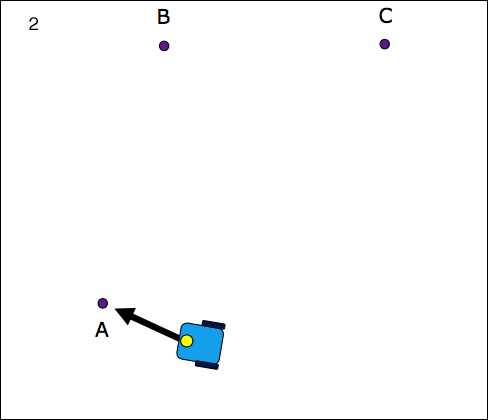
\includegraphics[width=0.32\textwidth, height=0.25\textwidth]{Figures/step2.png}
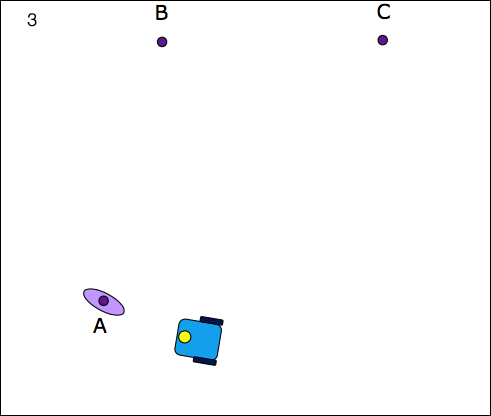
\includegraphics[width=0.32\textwidth, height=0.25\textwidth]{Figures/step3.png}
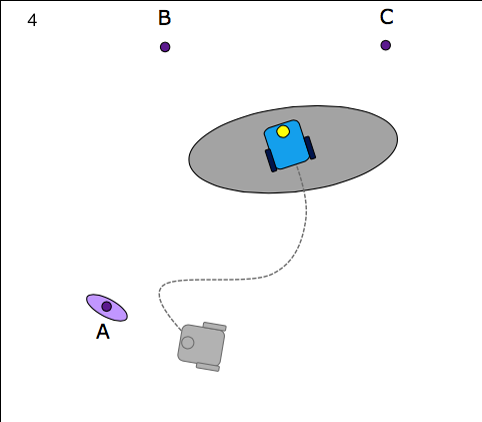
\includegraphics[width=0.32\textwidth, height=0.25\textwidth]{Figures/step4.png}
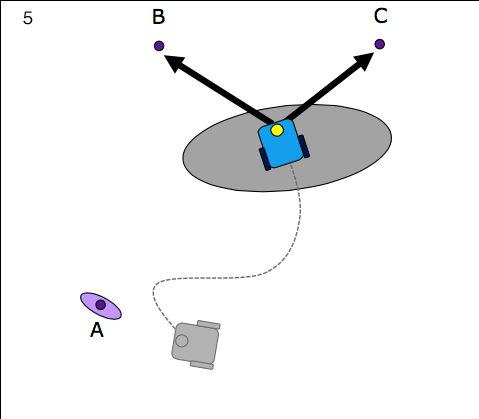
\includegraphics[width=0.32\textwidth, height=0.25\textwidth]{Figures/step5.png}
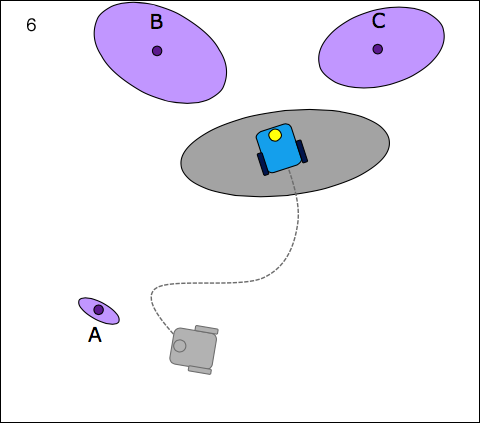
\includegraphics[width=0.32\textwidth, height=0.25\textwidth]{Figures/step6.png}
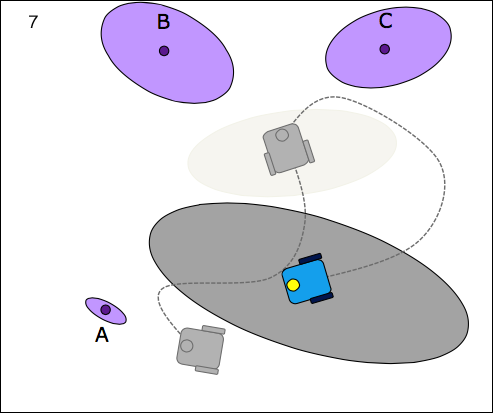
\includegraphics[width=0.32\textwidth, height=0.25\textwidth]{Figures/step7.png}
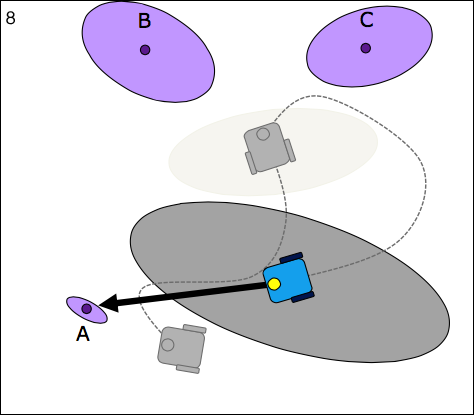
\includegraphics[width=0.32\textwidth, height=0.25\textwidth]{Figures/step8.png}
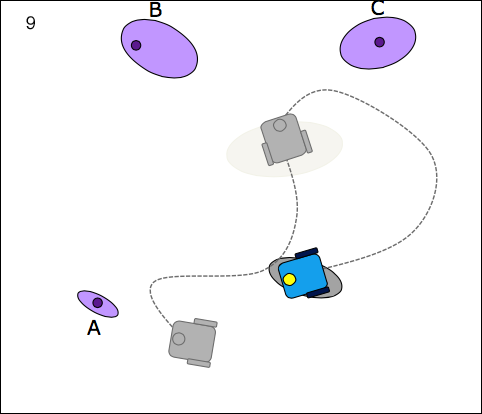
\includegraphics[width=0.32\textwidth, height=0.25\textwidth]{Figures/step9.png}
\caption{A basic representation of the SLAM procedure. Grey ellipses depict uncertainty regarding the robot's pose and purple ellipses depict uncertainty regarding the feature positions. Adapted from~\cite{step1}.}
\label{fig:slam}
%\end{center}
\end{figure}

\begin{table}[h]
\caption{Individual steps undertaken to solve the SLAM problem.}
%\begin{center}
\begin{tabular}{|l|l|}
\hline
Image & \multicolumn{1}{|c|}{Process} \\
\hline
$1-3$ & \pbox{15cm}{Robot begins exploration, observes feature A and updates the internal representation accordingly.}\\
\hline
$4$ & Robot moves, subsequently increasing uncertainty regarding its pose.\\
\hline
$5-6$ & \pbox{15cm}{Robot observes features B and C and updates the internal representation. Note that the increase in pose uncertainty yields a greater uncertainty in feature position due to the relationship between the robot's pose and the feature estimates.}\\
\hline
$7-8$ & \pbox{15cm}{Robot moves, again increasing uncertainty regarding its pose before re-observing old feature A. This is referred to as \textit{loop closure}.} \\
\hline
$9$ & \pbox{15cm}{Because the feature locations and robot's pose estimates are not statistically independent, the uncertainty regarding the pose as well as that of all feature positions decreases.}\\
\hline
\end{tabular}
%\end{center}
\label{tab:Slam}
\end{table}% 

\textit{A feature can also be referred to as a landmark and the aforementioned terms will from hereon in be used synonymously.}
%\newpage
%%%%%%%%%%%%%%%%%%%%%%%%%%%%%%%%%%%%%%%%%%%%%%%%%%%%%%%%%%%%%%%%%%%%%%%%%%           
%\subsubsection{Vision Based Approaches}
%Vision based approaches utilise the data captured from cameras. Camera's project the 3D features they observe in the world around them onto a 2D \textit{image plane}. Once projected, the 2D image is then digitised into pixel coordinates where they can then be interpreted, analysed and manipulated in software. There has been a great improvement in the quality of data captured by cameras in the past decade, allowing very reliable projections of the environment. Additionally, cameras are compact, reliable and relatively low-cost with respect to alternative sensors used in SLAM implementations.\\\\
%Camera systems can be configured in different ways to realise SLAM, utilising anything from a single camera to many calibrated cameras. Each configuration yields its unique advantages (as well as disadvantages) with successful published implementations existing for each configuration. The two most popular implementations include that of a single camera system and that of a stereo pair. Each of the aforementioned implementations are briefly described below along with their respective pros and cons: 
%\begin{enumerate}
%\item \textbf{Single Camera}\\
%Single camera systems (a.k.a monocular systems) rely on using the image data of a single camera only. Although there have been various successful implementations and variations using single camera systems~\cite{dav2007,ptam,visodom}, it remains an issue that the depth of a feature cannot be recovered from a single image. The utilisation of a single camera however, ensures a lower cost as well as a relatively simple SLAM realisation as apposed to that of alternative SLAM approaches.
%\item\textbf{Stereo Calibrated Camera Pair} 
%\\Stereo camera pairs utilise two identical cameras fixed at a given distance between them. These systems are able to effectively recover the depth of a feature in an image from a single observation, through matching a this feature across both images. The setup for such a system however, is somewhat complex as the individual cameras are required to be carefully calibrated. Additionally, stereo systems generally provide a greater computational and financial expense than that of a monocular system.   
%\end{enumerate}
%A meaningful comparison between the aforementioned algorithms is given by~\cite{comp}. 
\newpage
%%%%%%%%%%%%%%%%%%%%%%%%%%%%%%%%%%%%%%%%%%%%%%%%%%%%%%%%%%%%%%%%%%%%%%%%%%    
\subsection{Problem Description}\label{sec:into2}
A vision-based autonomous vehicle operating within an unknown and restricted environment requires a constant update regarding its \textit{current location}. Many autonomous systems have limited knowledge regarding the surrounding environment but may possess a sensor capable of observing the environment - in this case a camera(s). It is therefore essential that a solution to this specific localisation problem incorporates the ability to use sensor measurements to build a map on the fly while concurrently locating itself within the map. In a restricted environment, it is likely that a robot will return to a previously observed region, making it essential to incorporate robust \textit{repeatable} localisation where drift from ground truth can be corrected. % Cameras are easily accessible, relatively accurate sensors that are far less expensive than other sensors such as ultrasonic or laser rangefinder sensors. A vision-based solution that utilises a camera should therefore be considered.

Vision-based SLAM implementations as depicted in Figure~\ref{fig:slam} provide the necessary functionality to achieve repeatable localisation. SLAM algorithms utilising single cameras~\cite{dav2007,sola,ptam} have provided elegant yet accurate solutions to the SLAM problem, reconstructing accurate SLAM maps and subsequently achieving localisation. One such algorithm presented by Davison et al.~\cite{dav2007}, termed \textit{MonoSLAM}, allows for real-time repeatable localisation of a handheld camera moving within a restricted environment. MonoSLAM, along with the work succeeding it~\cite{dav2007,highspeed2008,scale2010,idp}, has achieved successful results in retrieving the trajectory of a robot, forming a persistent SLAM map and ultimately maintaining repeatable localisation. Although a map of features is not the desired outcome, it remains essential to solving the localisation problem. 

There are however, inherent disadvantages of a MonoSLAM system. Firstly, the utilisation of a single camera prohibits the system from immediately obtaining an accurate depth estimate. A feature is required to be observed from several different viewpoints before an accurate depth estimate can be made. Secondly, the motion model, namely a \textit{constant linear and angular velocity} model, constrains the movement of the system to ``smooth" trajectories - as depicted in Figure~\ref{fig:camvel}. If erratic forces or disturbances act upon the system, the pose of the robot is generally lost, and in most cases irrecoverable. Lastly, because there is no sufficient knowledge of the motion of the robot, the system is not well suited in certain practical scenarios. 
\begin{figure}[H]
\centering%\begin{center}
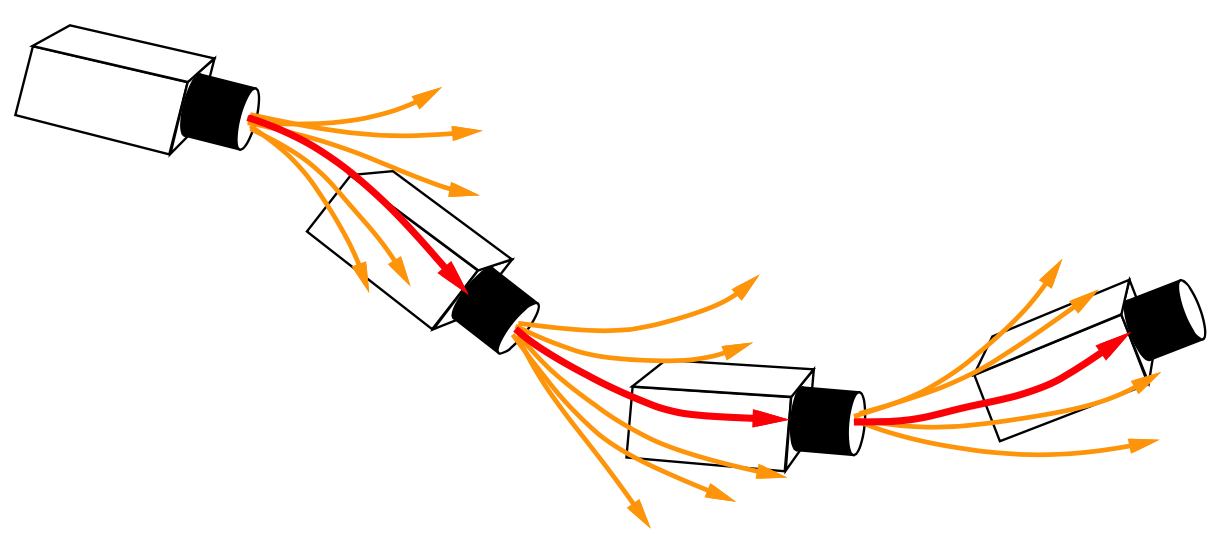
\includegraphics[width=0.48\textwidth, height=0.2\textwidth]{Figures/camvel.png}
\caption{Visualisation of the smooth trajectories of the constant linear and angular velocity model. Adapted from~\cite{dav2007}}
\label{fig:camvel}
%\end{center}
\end{figure}
Information obtained from additional sensors could potentially improve the disadvantages presented by MonoSLAM. Single camera SLAM implementations using information from an additional measurement sensor (e.g. a laser range finder), such as that presented in a study by Fu et al.~\cite{lasermono}, are not only too expensive but would be difficult to integrate with a single camera system from a modelling perspective. A more elegant solution that uses measurements to improve the motion estimates is required.   

To extend the range of practical applications of MonoSLAM, a motion model capable of estimating the pose of a robot due to a variety of movements is essential. The current constant linear and angular velocity model limits the robot to smooth movements and therefore needs to be adjusted or replaced. Using additional information can provide the current velocity motion model with more accurate state estimates, but cannot allow movements that aren't ``smooth". Davison et. al~\cite{dav2007}, confirms that additional information such as angular velocities obtained from a \textit{gyroscope} improve the state estimates, but cannot compensate for a change in motion dynamics. 

A \textit{kinematic estimator} directly measures the derivatives (first and second order) of the position and orientation of the robot as opposed to calculating them from the control inputs and the system's physical model. Inertial measurement units (IMU) can directly measure these derivates and typically comprise of an accelerometer and a gyroscope (and sometimes a magnetometer) that record the accelerations and angular velocities respectively. Incorporating such a subsystem could allow a wider variety of practical scenarios as the target system isn't constrained to a specific motion.
%%%%%%%%%%%%%%%%%%%%%%%%%%%%%%%%%%%%%%%%%%%%%%%%%%%%%%%%%%%%%%%%%%%%%%%%%%%
\subsection{Project Objectives}\label{sec:into3}
This project seeks to utilise the aforementioned MonoSLAM system of Davison et al. and improve the localisation thereof by using \textit{additional} sensor information. The improvement(s) of the system should allow the existing system to obtain better localisation and extend the range of applications upon which the system can be applied while maintaining the original performance standard: repeatable localisation at 30 Hz for approximately 100 features. The system should utilise a \textit{single} camera as the measurement sensor and preferably support real-time operation. All processing regarding the SLAM algorithm can be done on a standard PC that communicates with the sensors via a serial port. The project budget is R $1500.00$. The primary objectives of this project include:
\begin{itemize}
\item \textbf{Performing an overview on the current techniques used to realise SLAM} \\
In order to understand how SLAM is implemented, an understanding of probability theory and state estimation is required. These concepts - specifically recursive state estimation and the Bayes filter - need to be researched and analysed before choosing a suitable technique to implement.
\item \textbf{Analysis of the kinematic estimator as an alternative motion model}\\
A kinematic estimator is suggested as a alternative motion model. The kinematic estimator needs to be researched, mathematically derived and simulated. The results from the simulation should correspond to the mathematical derivation. The advantages and disadvantages of the kinematic estimator also need to be investigated.
\item \textbf{Hardware Design of the System} \\
The kinematic estimator requires additional measurements obtained from an IMU. The IMU is required to interface with the PC via a micro-controller. The micro-controller allows precise synchronisation between the images sampled by the camera and the IMU measurements. A functional diagram of the system's hardware components are depicted in Figure~\ref{fig:sys}. 
\item \textbf{Comparison between proposed and original MonoSLAM implementations}\\
If time allows, a set of tests are required to be derived and implemented to establish whether the proposed improvement(s) indeed satisfy the desired requirements.  
\end{itemize}
\begin{figure}[h]
%\begin{center}
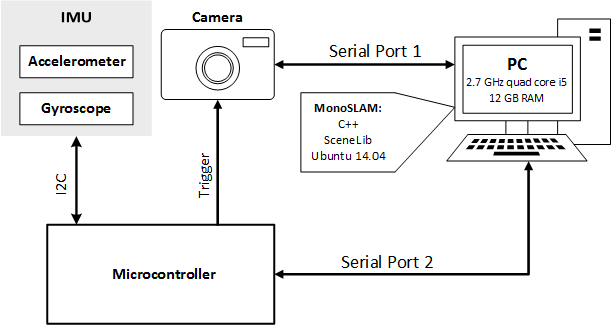
\includegraphics[width=\textwidth, height=0.45\textwidth]{Figures/Overview.png}
\caption{Diagram representing the interaction between the system's hardware and software components}
\label{fig:sys}
%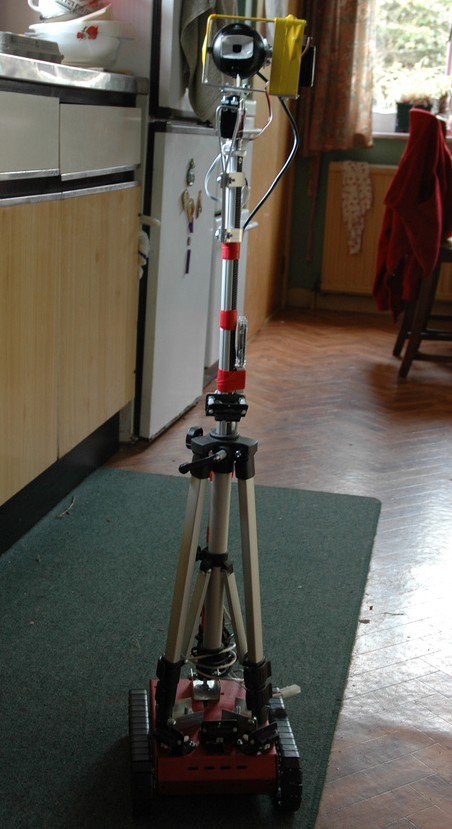
\includegraphics[width=\textwidth, height=0.5\textwidth]{Figures/rob.jpg}
%\end{center}
\end{figure}

%It is initially assumed that these measurements provide the necessary information to improve motion estimates. This project will primarily focus on deriving an accurate kinematic estimator as the motion model of a MonoSLAM system that incorporates inertial measurements to better approximate the trajectory of a robot. 
%An EKF (EKF) is chosen as the probabilistic method that realises the solution to the SLAM problem. The EKF is chosen for its simplicity to implement and because it is assumed that the Unscented KF (UKF)\textcolor{red}{[ref]} will only provide a greater efficiency if the number of landmarks are large. Considering that a restricted environment is being explored by the robot, it is expected as presented by Davison et al.~\cite{dav2007}, that the number of landmarks present in the SLAM map will not exceed 100. Furthermore it is assumed that a first order linearisation presents a good enough approximation for the modelling of the system dynamics. 

%The process regarding the construction of this map of features, namely that of recursive state estimation, is to be implemented through the use of an (Extended) KF. The map initially, completely void of any landmarks, is recursively updated according to the subsequent fusions of both the prediction and  the measurement presented to the KF. As new (potentially interesting) features are observed, the state estimates of both the camera as well as the landmarks are both updated - augmenting the state vector with additional features (if indeed they are observed) while deleting any landmarks that are no longer of interest. In order to obtain the best possible result, the algorithm should strive to obtain accurate state estimation regarding the movement of the robot as well as a sparse set of high-quality landmarks. Each of the steps regarding the realisation of the previously mentioned map of features are to be defined, described and analysed in the sections that follow. 
%The ultimate goal of any three dimensional (3D) SLAM approach, is to obtain a probabilistic 3D map of point features, representing at every time instance, the estimates of both the state of the robot as well as the positions of every feature observed. The previously mentioned features of interest are more commonly referred to as \textit{landmarks} and the aforementioned terms will, from hereon in, be used synonymously.  Most importantly though, the map is to contain the \textit{uncertainty} associated with each of the aforementioned estimates.\\ The past decade however, has yielded many acceptable and impressive solutions as in~\cite{highspeed2008, scale2010,srukf}, to the aforementioned requirements using a single camera, with the original proposal presented by Davison et al.~\cite{dav2007}, more commonly referred to as MonoSLAM (Monocular vision based SLAM). In MonoSLAM, the robot is set to \textbf{only} obtain sensor information through the utilisation of a singular camera system. There are however, inherent disadvantages of such a system: Firstly, the utilisation of a single camera prevents the system from immediately obtaining an accurate depth estimate. Landmarks are required to be examined from various viewpoints before an appropriate depth estimation can be concluded. Secondly, the motion model (namely a constant velocity model) constrains the movement of the system to smooth, constant trajectories. In the event that erratic, immediate disturbances act upon the system, the pose of the robot is generally lost, and in most cases irrecoverable. Lastly, because no sufficient knowledge regarding the movement of the robot exists - its practical application is vastly limited. \\The proposed approach to be presented in the following paper, aims to improve the system to limit of these disadvantages, namely the latter two. This paper aims to extend the aforementioned system of Davison with the utilisation of \textit{additional} sensor information regarding the robot's motion. An inertial measurement unit (IMU) will provide this additional information, recording the movement of the robot through space as a result of the control inputs to the system. The additional data allows the system to be modelled as a rigid, kinematic body upon which kinematic estimation can be applied. Inevitably, a kinematic estimator allows the system a greater knowledge of its movement - because it is being measured through inertial sensors.\\\\
%The process regarding the construction of this map of features, namely that of recursive state estimation, is to be implemented through the use of an (Extended) KF. The map initially, completely void of any landmarks, is recursively updated according to the subsequent fusions of both the prediction and  the measurement presented to the KF. As new (potentially interesting) features are observed, the state estimates of both the camera as well as the landmarks are both updated - augmenting the state vector with additional features (if indeed they are observed) while deleting any landmarks that are no longer of interest. In order to obtain the best possible result, the algorithm should strive to obtain accurate state estimation regarding the movement of the robot as well as a sparse set of high-quality landmarks. Each of the steps regarding the realisation of the previously mentioned map of features are to be defined, described and analysed in the sections that follow. 
%\newpage
%The intended contribution of this paper realises an improvement in not only the state estimation of the system, but localisation as a whole. Additionally the kinematic estimator embedded within the system should serve as a means to integrate the proposed system as part of a larger system regardless of that system's physical model.  Moreover, the proposed system is required to operate in real time at a rate of at least the 30 Hz for 100 landmarks; as achieved by Davison in his original work presented in \cite{dav2007}.  
%%%%%%%%%%%%%%%%%%%%%%%%%%%%%%%%%%%%%%%%%%%%%%%%%%%%%%%%%%%%%%%%%%%%%%%%%%
\subsection{Project Outline}
The remainder of this report is presented as follows:\\\\
\textbf{Chapter 2: Probabilistic State Estimation Techniques}\\
This chapter presents all of the necessary research to effectively design and implement a solution to the SLAM problem. This chapter focusses on introducing the reader to the basic theory pertaining to probability theory and recursive state estimation. The chapter further explains how recursive state estimation can be implemented to provide a solution(s) to the SLAM problem.\\\\
\textbf{Chapter 3: Design}\\
This chapter provides a detailed overview of MonoSLAM. The relevant variable representation and functional components are initially discussed. The chapter then seeks to derive the state transition probability model, now comprised of a kinematic estimator. An overview of the extended Kalman filter's measurement update is also given.\\\\
\textbf{Chapter 4: Implementation}\\
This chapter sets out to predict the behaviour of the various subsystems through simulation. The results from the analysis of the kinematic estimator, extended Kalman filter and inertial measurement unit are all analysed accordingly.\\\\
\textbf{Chapter 5: Testing and Results}\\
This chapter presents all the relevant tests carried out to determine the proposals validity. The results of these tests are subsequently analysed.\\\\
\textbf{Chapter 6: Conclusions and Recommendations}\\
This chapter provides a summary recommendations by the author that is applicable to future work. The final conclusion is formulated analysing the state of the final system compared to the objectives of the project. 
\newpage
%%%%%%%%%%%%%%%%%%%%%%%%%%%%%%%%%%%%%%%%%%%%%%%%%%%%%%%%%%%%%%%%%%%%%%%%%%    
%\section{Literature Study}
%\newpage
%%%%%%%%%%%%%%%%%%%%%%%%%%%%%%%%%%%%%%%%%%%%%%%%%%%%%%%%%%%%%%%%%%%%%%%%%%    
\section{Theory: Probabilistic State Estimation Techniques}
\subsection{Introduction}
The following chapter will provide a brief, yet concise introduction to the fundamental algorithms that are necessary to implement SLAM. The fundamental concepts, particularly the various techniques associated with the implementation thereof will be addressed. The goal of this section is to introduce the fundamental concepts as well as the mathematical and probabilistic principles that form the basis of state estimation in the robotics field of study.

Initially, the Bayes filter; that is the algorithm that forms the basis of all state estimation techniques presented in this report, will be introduced and formally discussed. Thereafter, the Gaussian Filter family - particularly the \textit{Kalman Filter} (KF) - as well as its variants - are to be introduced, discussed and defined in terms of the context of this project. It is worthwhile to note that theory in this chapter resembles material from the book Probabilistic Robotics by Thrun et al.~\cite{probrob} and is adapted therefrom for convenience.  
%This chapter provides a brief, yet concise introduction to the fundamental theoretical concepts and algorithms that are necessary to implement SLAM. Firstly, the concept of estimating state variables using a motion model and sensor measurements is initially described. The chapter then presents a suitable state estimation method, namely the Bayes filter. Additionally, the KF, a particular implementation of the Bayes filter is derived. Finally, the KF is appropriately extended to present the EKF, the state estimation algorithm chosen to realise this project.    

\subsection{Recursive State Estimation}\label{sec:state}
 %Quantities exist that are not directly observable, yet are still able to be obtained through sensor data. Sensors though, obtain limited data regarding certain quantities and most importantly, are affected and often corrupted by \textit{noise}.   
%Probabilistic robotics yields a unique yet fundamental concept at its core, that is: estimating a state through sensor data. \\
State variables define the mathematical state of a system's dynamics and describe the impact of the system's future behaviour in the absence of external factors. Although a robot's dynamics can be mathematically modelled, they have quantities that are not directly observable but can be obtained through sensor measurements. Sensors though, obtain limited data regarding certain quantities and most importantly, are corrupted by \textit{noise}.

State estimation then, seeks to recover state variables using measured sensor data, control inputs to the system as well as the system model. The value obtained is referred to as a \textit{state estimate}. In the case of SLAM, the state estimates of a robot incorporate the robot's pose as well the position of each landmark in the environment.  

\textit{Recursive state estimation} however, doesn't require the system to keep a complete history of \textit{all} measurements and control inputs, using only the current control inputs and measurements to update the previous state estimate. Probabilistic state estimation algorithms - to be investigated in this section - compute \textit{belief} distributions regarding state variables where the belief reflects a robot's internal knowledge of its state. 

In the case of SLAM, the robot is required to know its location at each time instance $t$. The belief must thus be calculated at each time step.  In order to achieve recursive state estimation, the state estimates of the robot should only incorporate the latest measurements. Additionally, the calculation of the belief should incorporate the previous estimates. Provided that the the system also obeys the Markov assumption - that previous data and future data are independent provided that the current state $\textbf{x}_t$ is known - the \textit{Bayes filter} provides such recursive state estimation. 
\newpage
%%%%%%%%%%%%%%%%%%%%%%%%%%%%%%%%%%%%%%%%%%%%%%%%%%%%%%%%%%%%%%%%%%%%%%%%%%
\subsection{Bayes filter}\label{sec:bayes}
The previously mentioned belief of a robot can be represented by a probability distribution that assigns a probability to each state outcome. The belief distribution is a posterior probability over the state variable that is conditioned over the measurements and control data~\cite{probrob}. Mathematically the belief with regard to a state variable $\textbf{x}_t$ is, as shown in the book Probabilistic Robotics by Thrun et al.~\cite{probrob}:     
%A key concept worth describing is the previously mentioned \textit{belief} of a robot. The belief represents the robot's understanding regarding the state of its own dynamics (its position, orientation etc.) as well as that of the surrounding environment. This critical concept proves a fundamental basis in probabilistic robotics. The belief can be represented as a conditional probability distribution whereby each possible scenario (state) is assigned a probability (density). 
\begin{equation} \label{eq:belief}
bel(\textbf{x}_t) = p(\textbf{x}_t\hspace{0.1cm}|\hspace{0.1cm}\textbf{z}_{1,..,t},\hspace{0.1cm}\textbf{u}_{1,..,t}).
\end{equation}

This describes, for a given time $t$, a joint density of the robot state as well as the landmark locations {given} all of the previously recorded observations ${z}_{1,..,t}$ and control inputs ${u}_{1,..,t}$.
%Considering that the state of the robot is constantly updated at every timestep $t$ and that each update is dependent upon the state at the previous timestep, it is essential that the algorithm required be recursive in nature. The \textit{Bayes filter} algorithm provides precisely such a procedure. The algorithm calculates the belief distribution stated in equation~\ref{eq:belief} from the observation and control data. 
Table~\ref{tab:KF} presents a pseudo-algorithm of the Bayes filter algorithm \cite{probrob}:

\begin{table}[h]
\centering%\begin{center}
\caption{The Bayes filter Algorithm} \label{tab:BF}
\begin{tabular}{l l l}
\hline
\textbf{Input}: &previous belief $bel(\textbf{x}_{t-1})$, control input(s) $\textbf{u}_t$, measurement(s) $\textbf{z}_t$\\ 
\textbf{Output}: &current belief $bel(\textbf{x}_{t})$\\
\hline
\hline
for all $\textbf{x}_t$: \\
1. & $\overline {bel}(\textbf{x}_t)$ = $\int p(\textbf{x}_t\hspace{0.1cm}|\hspace{0.1cm}\textbf{u}_{t},\hspace{0.1cm}\textbf{x}_{t-1})bel(\textbf{x}_{t-1})d\textbf{x}_{t-1}$ \\
2. & ${bel}(\textbf{x}_t)$ = $\eta p(\textbf{z}_t\hspace{0.1cm}|\hspace{0.1cm}\textbf{x}_{t})\overline {bel}(\textbf{x}_t)$ \\
3. &end for. \\
\hline\hline
\end{tabular}
%\end{center}
\end{table}%
The recursive nature of the algorithm can thus be seen from Table~\ref{tab:BF}; whereby the belief $\overline {bel}(\textbf{x}_t)$ at the current time $t$ is obtained through initially calculating the belief at the previous time step $t-1$. The Bayes filter contains two essential steps: \textit{prediction} (line 1) and \textit{measurement update} (line 2). The prediction step initially processes the control inputs before subsequently predicting the current belief based on the prior belief and the probability that a transition from $\textbf{x}_{t-1}$ to $\textbf{x}_t$ occurs. Thereafter, the measurement update improves the belief by adding information about the states, observed from new measurements. 

The Bayes filter can be implemented in many different ways, two of which are discussed later in the report. Upon choosing a suitable implementation, a trade off between the following properties needs to be made:
\begin{itemize}
\item Computational efficiency
\item Accuracy of the approximation 
\item Ease of Implementation
\end{itemize}
The Bayes filter provides a suitable solution through recursive state estimation. Additionally, the only approximation that is made upon deriving the Bayes filter is the Markov assumption. Along with its relatively simple implementation, the fact that no other approximations are made is why the Bayes filter is chosen as the solution to the SLAM problem in this project (and many others).
   
The mathematical derivation of the Bayes filter contains further technicalities. The techniques presented in this project require only a basic understanding of the Bayes filter. A detailed analysis of the Bayes filter can be obtained from the book Probabilistic Robotics by Thrun et al.~\cite{probrob}. 
%%%%%%%%%%%%%%%%%%%%%%%%%%%%%%%%%%%%%%%%%%%%%%%%%%%%%%%%%%%%%%%%%%%%%%%%%%
\newpage
\subsection{Gaussian Filters}\label{sec:Gausfil}
%%%%%%%%%%%%%%%%%%%%%%%%%%%%%%%%%%%%%%%%%%%%%%%%%%%%%%%%%%%%%%%%%%%%%%%%%%
Amongst the many different implementations of the Bayes filter are the \textit{Gaussian filter} family. The basic idea behind a Gaussian filter is that a belief can be represented as a multivariate Gaussian distribution, represented mathematically as follows~\cite{probrob}:
\begin{equation} \label{eq:normal}
p(\textbf{x}_t)=\cfrac{1}{\sqrt{|2\pi\boldsymbol{\Sigma}|}}\hspace{0.1cm}\text{exp}\hspace{0.1cm}\bigg\{-\frac{1}{2}(\textbf{x}_t-\boldsymbol{\mu})^T\boldsymbol{\Sigma}^{-1}(\textbf{x}_t-\boldsymbol{\mu})\bigg\},
\end{equation} 
where the density across the state variable $\textbf{x}_t$ is characterised through two fundamental parameters: the mean $\boldsymbol{\mu}$ and the covariance $\boldsymbol{\Sigma}$. Such a parameterisation is known as the \textit{moments parameterisation} (as the mean and covariance represent the first and second order moments respectively). This parameterisation allows a number of recursive filter algorithms to be derived, two of which are examined in this project: the \textit{Kalman filter} (KF) and its non-linear counterpart, the \textit{extended Kalman filter} (EKF). It is important to realise that both of the aforementioned filters belong to the same sub-class of filters - namely the KF Family - and therefore most of the fundamental concepts and functionality between them are identical. Each filter is discussed in further detail in the subsections that follow.   
%%%%%%%%%%%%%%%%%%%%%%%%%%%%%%%%%%%%%%%%%%%%%%%%%%%%%%%%%%%%%%%%%%%%%%%%%%
\subsubsection{Kalman Filter} \label{sec:KF}
Probably the most fundamental of all Gaussian filter algorithms, is the \textit{Kalman filter}. Introduced in a study presented by Kalman~\cite{kalman}, the KF can be briefly described as an optimal estimator. It remains a popular technique for filtering and prediction of \textit{linear} systems that contains Gaussian uncertainty. The KF seeks to describe a belief distribution of a state variable $\textbf{{x}}_t$ as described in Equation~\ref{eq:normal}. Subsequently, the state vector $\textbf{{x}}_t$ is modelled by a single multivariate Gaussian distribution with a mean $\boldsymbol{\mu}_t$ and covariance $\boldsymbol{\Sigma}_t$, at each time instance $t$ (while previous time steps are denoted as $t-1$, $t-2$, etc.). The general implementation as described above though, is only valid provided that the following three properties hold true - as listed in~\cite{probrob}: 
\begin{enumerate}
\item The state transition model probability \textbf{must} be a \textit{linear} function with additive Gaussian (process) noise. %The state transition model probability is shown according to Thrun et al.\cite{probrob}:\\
\begin{equation}\label{eq:SSmodelg}
g(\textbf{u}_{t}, \textbf{x}_{t-1}) :  \textbf{x}_t = \textbf{A}_t\textbf{x}_{t-1} + \textbf{B}_t\textbf{x}_t + \textbf{w}_t.
\end{equation}
\item The observation model probability \textbf{must} be a \textit{linear} function with additive Gaussian (sensor) noise. %The observation model probability is shown according to Thrun et al.\cite{probrob}:\\
\begin{equation}\label{eq:SSmodelh}
h(\overline{\boldsymbol{\mu}}_t) : \textbf{z}_t = \textbf{C}_t\textbf{x}_t + \textbf{v}_t,
\end{equation}
where $\textbf{w}_t$ and $\textbf{v}_t$ represent process and sensor noise respectively.
\item The initial belief $bel(\textbf{x}_0)$ must be normally distributed.
\end{enumerate}
%In the context of Simultaneous Localisation and Mapping (SLAM), a KF algorithm seeks to determine the \textbf{optimal} trade off between the state of the robots pose and the position of the landmarks within the map - given process and measurement noise.\\
%provided that the state vector $\textbf{\^{x}}_k$, and landmark locations $\textbf{\^{y}}_{n,k}$ are modelled by a single multivariate Gaussian distribution. The system is to be observed at discrete steps in time - denoted by the subscript$k =1, 2,  3, ...$ - where at every individual timestep, it can be influenced by a set of actions. It is assumed that\\  

%Moreover, the solution to this specific implementation of the SLAM problem, takes a probabilistic form where the belief with regard to state variable $\textbf{x}_t$ is denoted as shown in equation~\ref{eq:belief}:
%\begin{equation}
%bel(\textbf{{x}}_t) = p\big(\textbf{{x}}_t\hspace{0.15cm}|\hspace{0.15cm}\textbf{z}_{1:t},\textbf{u}_{1:t}\big),
%\end{equation}

%with the aforementioned distribution described at every discrete time instance $t$.\\ A brief description would yield that the distribution above, describes, for a given time instance $t$, a joint density of the robot state as well as the landmark locations \textbf{given} all of the previously recorded observations, $\textbf{z}_{1:t}$ and control inputs, $\textbf{u}_{1:t}$.\\
The input to the KF is the belief $\overline{bel}(\textbf{x}_t)$ at time $t-1$, represented by $\boldsymbol{\mu}_{t-1}$ and $\boldsymbol{\Sigma}_{t-1}$. The KF requires a control input $\textbf{u}_t$ and a measurement $\textbf{z}_t$ at time $t$ to update the belief. Like the Bayes filter, the KF too is executed in two (sequential) steps: the \textit{control update step} and the \textit{measurement update step}. 

At time $t$, the prediction step aims to calculate a predicted belief $\overline{bel}(\textbf{x}_t)$ represented by $\overline{\boldsymbol{\mu}}_{t}$ and $\overline{\boldsymbol{\Sigma}}_{t}$. The predicted belief is modelled by a deterministic version of the state transition probability (Equation~\ref{eq:SSmodelg}) that incorporates the control input $\textbf{u}_t$ to the mean and covariance estimates. The update step aims to obtain the belief $bel(\textbf{x}_t)$ from the predicted belief $\overline{bel}(\textbf{x}_t)$ by incorporating the measurements $\textbf{z}_t$. The KF computes a Kalman gain, that determines the influence of a measurement in the new state estimate. The update step of the incorporates a product of two Gaussian probabilities. This product results is a new Gaussian with a weighted \textit{optimal} mean. The Kalman gain is thus optimal and is used to update the mean and covariance estimates such that the resulting belief distribution is optimal. An illustration of the weighted mean is depicted in Figure~\ref{fig:weight}:
\begin{figure}[H]
\centering%\begin{center}
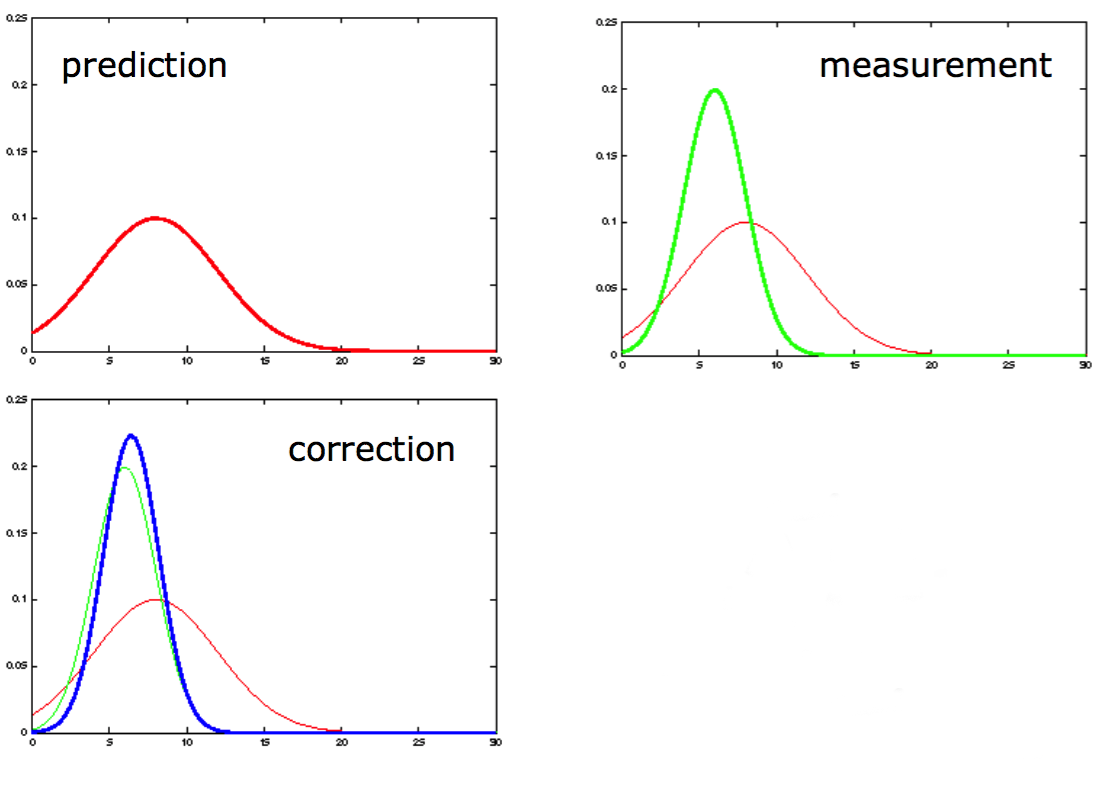
\includegraphics[width=0.8\textwidth, height=0.5\textwidth]{Figures/weight.png}
\caption{A graphical illustration of how the weighted mean is obtained. The correction (blue) is the product of the prediction (red) and measurement (green) Gaussian PDF's. Adapted from~\cite{cyril}.}
\label{fig:weight}
%\end{center}
\end{figure}
Each of the aforementioned steps are later discussed in more detail - with reference to implementations specific to this paper. Table~\ref{tab:KF} below, presents a pseudo-algorithm of the KF~\cite{probrob}:
% estimate the state into which the system will be transitioned from the previous state estimate ($\boldsymbol{\mu}_{t-1}$, $\boldsymbol{\Sigma}_{t-1}$) as a result of a set of internal and/or external dynamics to the system. These dynamics are typically described through the state transition function $g(\textbf{u}_t, \boldsymbol{\mu}_{t-1})$. Once an estimate is obtained for the transitioned state estimate ($\boldsymbol{\bar \mu}_t$, $\boldsymbol{\bar \Sigma}_t$), a measurement prediction is made in order to provide the expected measurements provided that the system were to find itself within the estimated transitioned state. These measurements are obtained through an observation model which has a function $h(\boldsymbol{\bar \mu}_t)$. Thereafter, an actual measurement, $\textbf{z}_t$ is then obtained through the system sensors in order to determine the actual state of the system ($\boldsymbol{\mu}_t$, $\boldsymbol{\Sigma}_t$). Ultimately, the actual state of the system and the previously predicted state are then compared with one another in order  to obtain the (optimally weighted) \textit{Kalman gain}: This 

\begin{table}[h]
\begin{center}
\caption{The KF Algorithm}\label{tab:KF}
\begin{tabular}{l l l}
\hline
\textbf{Input}: &previous mean $\boldsymbol{\mu}_{t-1}$ and covariance $\boldsymbol{\Sigma}_{t-1}$, control inputs $\textbf{u}_t$, measurements $\textbf{z}_t$\\ 
\textbf{Output}: &mean $\boldsymbol{\mu}_{t}$, covariance $\boldsymbol{\Sigma}_{t}$\\
\hline
\hline
&\textbf{Control update step} \\
\hline
1. & $\boldsymbol{\bar \mu}_{t}$ = $g(\textbf{u}_{t}, \boldsymbol{\mu}_{t-1})$ = $\textbf{A}_t\hspace{0.05cm}\boldsymbol{\mu}_{t-1} + \textbf{B}_t\hspace{0.05cm}\boldsymbol{\mu}_t$ + $\textbf{w}_t$\\
2. & $\boldsymbol{\bar \Sigma}_t = \textbf{A}_t \boldsymbol{\Sigma}_{t-1} \textbf{A}_t^T + \textbf{R}_{w,t}$ \\
\hline
&\textbf{Measurement update step}\\
\hline
3. & $\textbf{K}_t = \boldsymbol{\bar \Sigma}_{t} \textbf{C}_t^T (\textbf{C}_t \boldsymbol{\bar \Sigma}_{t} \textbf{C}_t^T + \textbf{R}_{v,t})^{-1}$ \\
4. & $\boldsymbol{\mu}_t = \boldsymbol{\bar \mu}_t + \textbf{K}_t[\textbf{z}_t-\textbf{C}_t\boldsymbol{\bar \mu}_t]$\\  
5. & $\boldsymbol{\Sigma}_{t} = (\textbf{I}-\textbf{K}_t \textbf{C}_t)\boldsymbol{\bar \Sigma}_t$ \\
\hline\hline
\end{tabular}
\end{center}
\end{table}%

The KF is generally considered an efficient algorithm for sparse sets. The \textit{computational complexity} of a matrix inversion is bounded by an order of $O(d^{2.8}+n^2)$~\cite{probrob}, where $d$ represents the dimensions of the measurements vector $\textbf{z}_t$ and $n$ the state space.  
%%%%%%%%%%%%%%%%%%%%%%%%%%%%%%%%%%%%%%%%%%%%%%%%%%%%%%%%%%%%%%%%%%%%%%%%%%
\newpage
\subsubsection{Extended Kalman Filter} \label{sec:EKF}
Considering that most practical systems of interest are non-linear, the KF in its purest form cannot be successfully implemented upon most modern day systems - including SLAM. Non-linear transformations of Gaussian random variables (RV) result in a different RV while any linear transformation of a Gaussian random variable yields another \textbf{different} Gaussian variable. This violates the important condition of the KF algorithm. This phenomenon can be illustrated through Figure~\ref{fig:lin}: % where a linear transform yields a transformed Gaussian RV and a non linear transform yields a RV with a different probability density:

\begin{figure}[h]
%\begin{center}
\includegraphics[width=0.49\textwidth, height=0.7\textwidth]{Figures/LIN1.png}
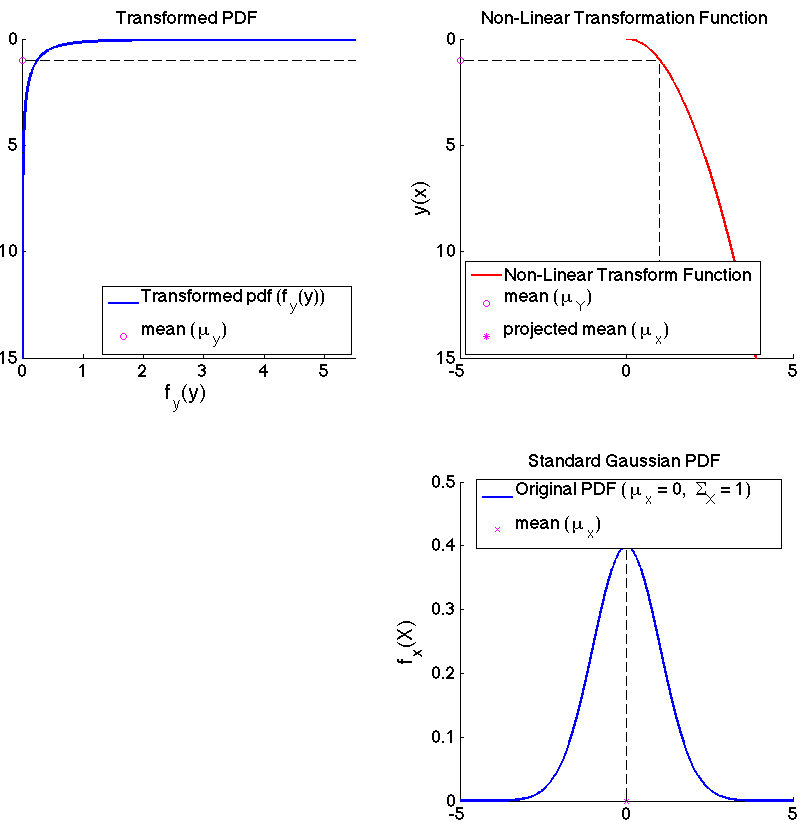
\includegraphics[width=0.49\textwidth, height=0.7\textwidth]{Figures/Non1.png}
\caption{Left: Linear transformation of a Gaussian random variable. Right: Non-linear transformation of a Gaussian random variable.}
\label{fig:lin}
%\end{center}
\end{figure}
%\begin{figure}[h]
%\begin{center}
%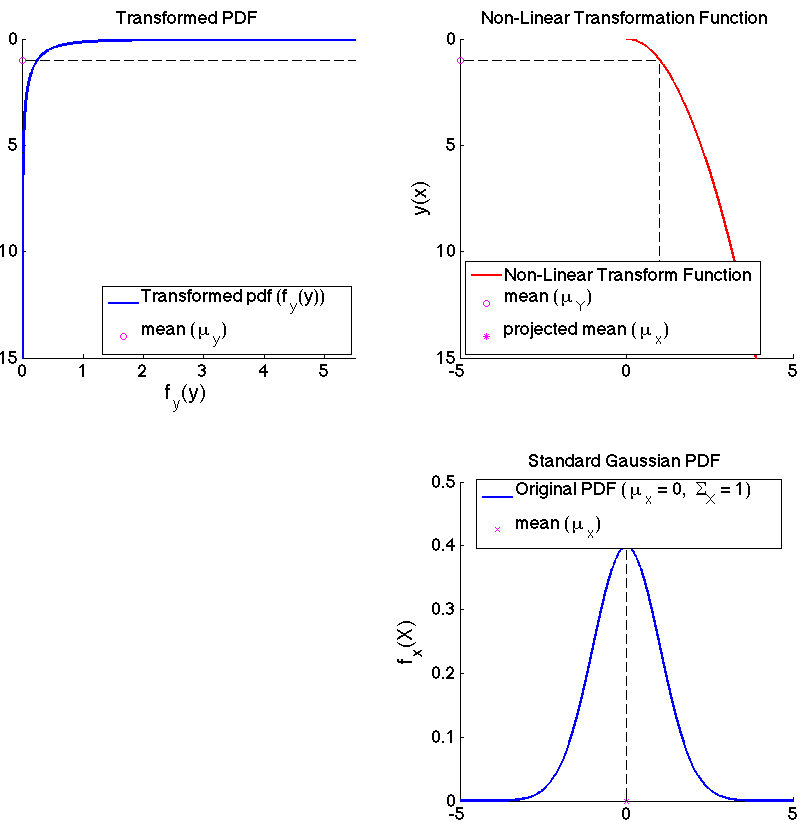
\includegraphics[width=0.49\textwidth, height=0.6\textwidth]{Figures/Non1.png}
%\caption{ Non-linear transformation of a Gaussian random variable.}
%\label{fig:non}
%\end{center}
%\end{figure}
The \textit{extended Kalman filter (EKF)}, an extension of the general KF, aims to enable the modelling of non-linear systems through local linearisation. As previously mentioned, the state transition function $g(\textbf{u}_t, \textbf{x}_{t-1})$, as well as the observation model $h(\textbf{x}_{t-1})$ of most practical systems are typically both non-linear in nature. These are typically only moderate non-linearities. Considering the aforementioned statement; it is necessary to determine a method for approximating a non-linear function as a linear function, more commonly referred to as linearisation. The linearisation process of EKF aims to linearise these functions so that the fundamental operations of the KF algorithm remain valid.

The linearisation process approximates an arbitrary non-linear function $k$ by a linear function that is \textit{tangent} to $k$ at the mean value of the Gaussian, $\boldsymbol{\mu}$. If the Gaussian is then projected through this new linear approximation, the resultant transformation would yield a random variable that is Gaussian in nature (as in Figure~\ref{fig:lin}). This technique is applied to both the state transition and observation functions. Many methods exist for linearisation of non-linear functions, but the EKF utilises the method of (first order) \textit{Taylor expansion}. The Taylor expansion creates a linear approximation of a non linear function, say $k$, by its own value as well as that of its gradient $k'$. The tangent of $k$ can be depicted by its partial derivative with respect to the state vector $\textbf{x}_{t-1}$:
\begin{equation}\label{eq:par}
k'(\textbf{x}_{t-1}, \textbf{u}_t) := \frac{\partial k(\textbf{x}_{t-1}, \textbf{u}_t)}{\partial \textbf{x}_{t-1}}.
\end{equation}

The argument of the function $f$ is chosen as the most likely point at the linearisation instance. For Gaussians, the most likely point is the mean $\boldsymbol{\mu}_{t-1}$. The linear approximation of the function $k$ can then be achieved through the linear extrapolation evaluated at its most likely point $\boldsymbol{\mu}_{t-1}$:
\begin{equation}\label{eq:app}
\begin{split}
k(\textbf{x}_{t-1}, \textbf{u}_t) &\approx f(\textbf{x}_{t-1}, \textbf{u}_t) + k'(\textbf{u}_{t},\boldsymbol{\mu}_{t-1})(\textbf{x}_{t-1}-\boldsymbol{\mu}_{t-1}) \\
&= k(\textbf{x}_{t-1}, \textbf{u}_t) + \textbf{K}_t^{\textbf{x}_{t-1}}(\textbf{x}_{t-1}-\boldsymbol{\mu}_{t-1})
\end{split},
\end{equation}
where $\textbf{K}_t^{\textbf{x}_{t-1}} = k'(\textbf{u}_{t},\textbf{x}_{t-1})$ is the \textit{Jacobian} matrix. 

It is important to note that {Jacobian} matrix is determined at each linearisation instance (each individual time step) as its parameters differ from one linearisation instance to the next. 

%Once linearisation is achieved, the EKF which behaves otherwise identically in terms of operation to the general KF, can be implemented upon non-linear systems. 
It is very important to note that because only a first order Taylor expansion is used to \textit{approximate} the linearisation, severe non-linearities will prohibit acceptable approximations of the Gaussian distribution upon transformations. If the linearisation point is chosen at a point close to the mean, the EKF will yield an acceptable approximation from the linearisation process. 

There are other variants of the KF that aren't discussed in this project, but have been carefully considered. It is assumed that the first order Taylor approximation provides a suitable approximation of the non-linearities that are expected in the system, namely the uncertainty regarding angle orientation errors. The \textit{Unscented KF} is assumed to be a less appropriate choice of filter to the EKF considering the the lack of severe system non-linearities. The objective of this project seeks to provide localisation for a set of approximately 100 landmarks. The \textit{Information Filter} will only provide a better computational complexity than the EKF if the number of landmarks are much larger. This analysis suggests that the EKF provides a suitable yet simple implementation of the Bayes filter.%The EKF is chosen as a suitable implementation of the Bayes filter as the non-linearities the first order Taylor approximation is poor due to severe non-linearities. This project however, assumes that the the number of landmarks aren't large enough for the UKF to provide a better efficiency and that the transition and measurement probabilities are reasonably approximated by the Taylor expansion. 

Table~\ref{tab:EKF}  below, systematically and mathematically represents the steps associated with the EKF~\cite{probrob}:

\begin{table}[h]
%\begin{center}
\caption{The EKF Algorithm}\label{tab:EKF}
\begin{tabular}{l l l}
\hline
\textbf{Input}: &previous mean $\boldsymbol{\mu}_{t-1}$ and covariance $\boldsymbol{\Sigma}_{t-1}$, control inputs $\textbf{u}_t$, measurements $\textbf{z}_t$\\ 
\textbf{Output}: &mean $\boldsymbol{\mu}_{t}$, covariance $\boldsymbol{\Sigma}_{t}$\\
\hline
\hline
&\textbf{Control update step} \\
\hline
1. & $ \boldsymbol{\bar \mu}_t$ = $g(\textbf{u}_t,  \boldsymbol{\bar \mu}_{t-1})$ \\
2. & $\boldsymbol{\bar \Sigma_t} = \textbf{G}_t^{x_{t-1}} \boldsymbol{\bar \Sigma_{t-1}} {\textbf{G}_t^{x_{t-1}}}^T + \textbf{R}_{w,t}$ \\
\hline
&\textbf{Measurement update step}\\ 
\hline
3. & $\textbf{K}_t = \boldsymbol{\bar \Sigma_{t}} {\textbf{H}_t^{x_{t-1}}}^T (\textbf{H}_t^{x_{t-1}} \boldsymbol{\bar \Sigma_{t}} {\textbf{H}_t^{x_{t-1}}}^T + \textbf{R}_{v,t})^{-1}$ \\
4. & $\boldsymbol{\mu_t} = \boldsymbol{\bar \mu}+ \textbf{K}_t[\textbf{z}_t-h(\boldsymbol{\bar \mu})]$\\  
5. & $\boldsymbol{\Sigma}_{t} = (\textbf{I}-\textbf{K}_t {\textbf{H}_t^{x_{t-1}}}^T)\boldsymbol{\bar \Sigma_t}$ \\
\hline\hline
\end{tabular}
%\end{center}
\end{table}%  
%%%%%%%%%%%%%%%%%%%%%%%%%%%%%%%%%%%%%%%%%%%%%%%%%%%%%%%%%%%%%%%%%%%%%%%%%%
\newpage
\section{System Overview}\label{sec:system}
%%%%%%%%%%%%%%%%%%%%%%%%%%%%%%%%%%%%%%%%%%%%%%%%%%%%%%%%%%%%%%%%%%%%%%%%%%
\subsection{Introduction}
This chapter sets out to provide an overview of the MonoSLAM algorithm. Initially, a general overview of MonoSLAM is given, stating the problem, previous work done regarding this problem and the limitations imposed on this work. Thereafter, the adequate state representation will be shown along with the required modelling of the measurement sensors. Finally, a complete analysis of the \textit{control update} and an overview of the \textit{measurement update} will be given.
%Initially, the adequate state representation of the system at hand will be denoted, whereby the components of the state vector - namely the camera position and cartesian feature states - will be defined and discussed. Additionally, the affect of the proposed extension - namely the IMU measurements as the control inputs to the system - will be properly defined and described. Furthermore, this section will seek to use the aforementioned definitions to completely define the two sequential steps required to successfully implement the EKF, namely the \textit{prediction} and \textit{update} steps. 
\begin{figure}[H]
%\begin{center}
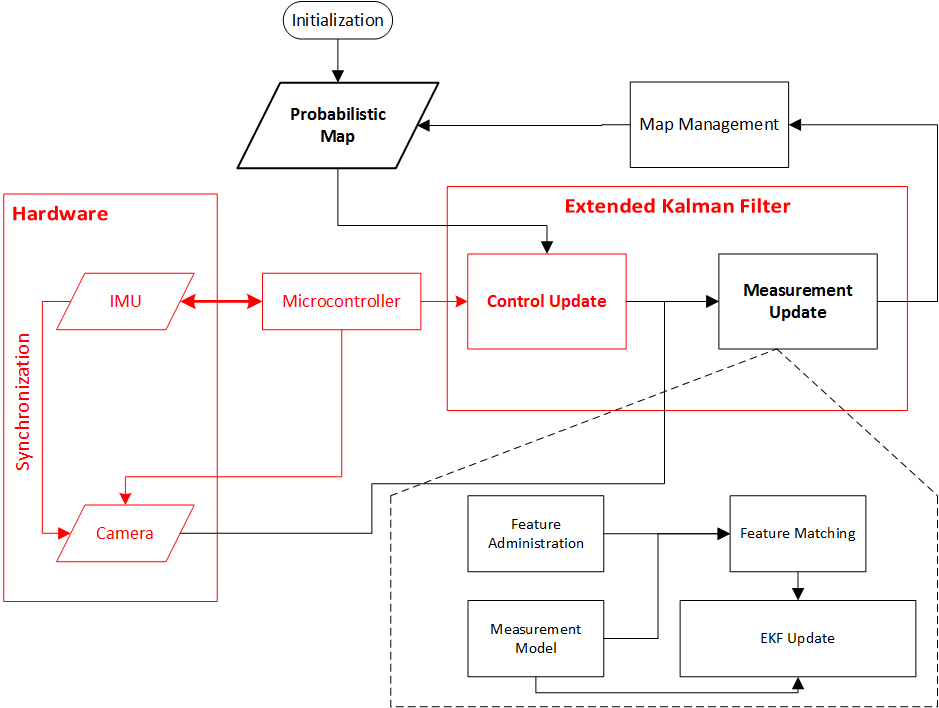
\includegraphics[width=\textwidth, height=0.67\textwidth]{Figures/Entier_System.png}
\caption{Functional diagram of the complete SLAM system. The sections in red depict the subsystems that have been accordingly altered or replaced in the implementation proposed in this project. The dashed lines show the internal processes of the measurement update - initially this is not trivial.}
\label{fig:system}
%\end{center}
\end{figure}

\subsection{MonoSLAM}
Originally presented in a study by Davison et al.~\cite{dav2007}, MonoSLAM provides suitable real-time and repeatable localisation using a single camera SLAM implementation. In MonoSLAM, the robot (typically a handheld camera) assumes a constant linear and angular velocity motion model, using the images from the camera to correct the state estimates. MonoSLAM is not the only successful implementation of single camera SLAM. Separate studies presented by Sola~\cite{sola} and Klein~\cite{ptam} respectively show alternative solutions to the single camera SLAM problem. Davison et al.~\cite{dav2007} however, provides the source code of MonoSLAM, a \textit{modular} system, under the GNU version 3 license so that possible improvements, such as those presented in this project, can be practised. This modularity and apparent ease of implementation as opposed to the particle filter based implementations presented by the alternative methods suggest MonoSLAM as an appropriate choice. 

MonoSLAM differs from other SLAM implementations in that it has no observable control inputs or other odometry. The system itself (a handheld camera) has no prior information of the users movements. Instead, the users movements are statically modelled through a constant linear and angular velocity model that expects linear and angular accelerations of a Gaussian profile. Incorporating additional measurements of the motion of the robot doesn't violate the methodology of MonoSLAM. The system still contains no prior information regarding its movement, but rather incorporates a control input equivalent that measures the movement.

Figure~\ref{fig:system} depicts a functional diagram of the proposed MonoSLAM system. The sections in red have been added/or altered from the original MonoSLAM implementation. This project seeks to utilise a kinematic estimator as an alternative to the current velocity and angular velocity motion model incorporated within the control update. The kinematic estimator will measure the angular velocities and linear accelerations of the robot from an inertial measurement unit as opposed to calculating them from physical models.  

The remaining components of the proposed approach presented in this study are identical to that of the MonoSLAM implementation: that is, using an EKF where the measurement update of the EKF depends on the measurements from a single camera. 

This particular vision based approach aims to use salient image \textit{patches} as long term landmarks as presented in \cite{dav2007,actvis}. These aforementioned patches are typically 11 $\times$ 11 pixels and are obtained through the image detection operator of Shi and Tomasi~\cite{shitom} from raw monochrome (greyscale) images. The goal is to repeatedly re-identify these image template patches over time after considerable camera movements. Invariably, basic 2D template matching algorithms are of little use, considering that any particular movements of the camera (even minimal) can severely alter the shape of a saved template patch. As a result, MonoSLAM assumes that each patch lies on a locally planar surface and that the surface normal is parallel to the vector from the feature to the camera at the instance that it is initialised. Once the depth of a patch has been determined - this is done through a small particle filter - the patch is stored to be used as a long term landmark. MonoSLAM stores these patches to provide a template for matching against a newly obtained 2D image at a later stage. Because the patches are never updated and remain in memory, long term localisation is possible. The \textit{innovation search} in Figure~\ref{fig:system} uses the measurement model to obtain a search area around which the system expects an initialised feature should be.

With regard to the management of the probabilistic map, it remains essential to the SLAM algorithm that decisions regarding the identification and deletion of landmarks be accurate and efficient. MonoSLAM's map-maintenance criterion demands that 12 reliable ``good" features be visible within the camera's field of view in order to maintain accurate localisation. A good feature implies that a feature remains visible within the camera's field of view. A new feature is initialised using the image operator of Shi and Tomasi~\cite{shitom} upon a box of pixels (80 $\times$ 60 pixels) placed within an image. This box position is chosen at random with the constraints that it shouldn't overlap with any existing features and that it remains in the camera's field of view. If a visible feature is unsuccessfully matched more than 50\% of the time, the landmark is deleted. It must be stressed that the aforementioned methods regarding vision based MonoSLAM measurements and map-management are described and implemented in this project exactly as they are in ~\cite{dav2007}. 

%The ultimate goal of the approach presented here, is to obtain a probabilistic three dimensional (3D) map of features, representing at every time instance, the estimates of both the state of the camera as well as the cartesian positions of every feature observed. This scenario is one approach of the previously discussed SLAM problem. Such a problem, is typically solved through the utilisation of the EKF. The goal of a single camera based SLAM algorithm (Monocular vision based SLAM), is to ultimately realise the objective of obtaining the aforementioned probabilistic map, through the utilisation of a single camera as achieved by Davison et al.~\cite{dav2007}. Various \textbf{successful} SLAM algorithms exist that utilise sensors other than cameras (laser range finders, ultrasonic sensors etc.)~\cite{2dlaser,ultra,lidar}. 

%Cameras though, prove a capable yet economical alternative to these sensors. Another successful and popular SLAM implementation is stereo vision (two calibrated cameras), yet the obvious disadvantage regarding such an approach is that double the cost is required as opposed to a single camera approach. Also, the calibration setup of a stereo vision system is generally quite complex. \\  

%It can be argued though, that the general approach presented in~\cite{dav2007} - more commonly referred to as \textit{MonoSLAM} - as well as the variants thereof ~\cite{idp,scale2010,highspeed2008,sola} can be improved through the utilisation of additional information regarding the motion of the robot. As previously discussed, the MonoSLAM system utilises a single camera as its only sensor. Apart from the inability to immediately estimate depth, a MonoSLAM system possesses no knowledge regarding its movement. The approach presented in this paper then, seeks to utilise exactly such information through the utilisation of an inertial measurement unit (IMU) as an extension to the original implementation. IMU's have been successfully implemented in SLAM based systems before, as implemented in ~\cite{IMU}. With the addition of an IMU, information regarding the changes in movement and orientation of the camera (namely the linear accelerations and the angular velocities) can be obtained and directly \textit{observed}. Ultimately, the stochastic constant velocity motion model of the general MonoSLAM algorithm can then be replaced with a kinematic estimation based motion model - one that is initially assumed to be more accurate - as it contains a considerably larger amount of information directly associated with a robot's movement.\\\\ 

%
%%%%%%%%%%%%%%%%%%%%%%%%%%%%%%%%%%%%%%%%%%%%%%%%%%%%%%%%%%%%%%%%%%%%%%%%%%
\newpage
\subsection{State Representation}
With reference to Chapter~\ref{sec:state}, state variables represent the mathematical ``state" of system. In order to calculate a belief distribution, the system must possess a model to predict future states. This model previously introduced as the state transition probability is commonly referred to as the \textit{motion model}. All relevant states are embedded within the state vector $\textbf{{x}}_t$. The state vector is defined at each timestep and consists of the robot's \textit{actual} pose and the \textit{actual} landmark positions within the map.\\
Mathematically, the probabilistic map is typically represented as a state \textit{estimate} that consists of a mean state vector $\boldsymbol{\mu}_t$ and a covariance matrix $\boldsymbol{\Sigma}_{t}$, represented at each time instance $t$. The mean state vector is a single column vector containing the means of the estimates of the robot as well as the landmark positions, and the covariance matrix is a square matrix containing the covariances of each state estimate with respect to every other state estimate. These quantities can be mathematically shown according to the book Probabilistic Robotics by Thrun et al.~\cite{probrob}:

\begin{equation}
\boldsymbol{\mu}_t = 
 \begin{pmatrix}
  \textbf{\^{x}}_{v,t}\\
  \textbf{\^{y}}_{1,t} \\ 
  \textbf{\^{y}}_{2,t} \\
  \vdots \\
  \textbf{\^{y}}_{n,t}
 \end{pmatrix} , \hspace{0.5cm}
\boldsymbol{\Sigma}_{t} =
 \begin{pmatrix}
  {\Sigma}_{x,x} & {\Sigma}_{x,{y_1}} & {\Sigma}_{x,{y_2}} & \cdots & {\Sigma}_{x,{y_N}} \\
  {\Sigma}_{{y_1},x} & {\Sigma}_{{y_1},{y_1}} & {\Sigma}_{{y_1},{y_2}} & \cdots &  {\Sigma}_{{y_1},{y_N}} \\
  {\Sigma}_{{y_2},x} & {\Sigma}_{{y_2},{y_1}} & {\Sigma}_{{y_2},{y_2}} & \cdots &  {\Sigma}_{{y_2},{y_N}} \\
  \vdots  & \vdots  & \vdots & \ddots & \vdots  \\
  {\Sigma}_{{y_n},x} & {\Sigma}_{{y_n},{y_1}} & {\Sigma}_{{y_n},{y_2}}& \cdots & {\Sigma}_{{y_n},{y_N}}
 \end{pmatrix}.
\end{equation}
These quantities then allow us to approximate the uncertainty regarding the generated feature map as a $N$-dimensional single multi-variate Gaussian distribution, where $N$, as stated above, is the total number of state estimates within the state vector and $n$ is the total number of landmarks within the map.
%%%%%%%%%%%%%%%%%%%%%%%%%%%%%%%%%%%%%%%%%%%%%%%%%%%%%%%%%%%%%%%%%%%%%%%%%%
\subsubsection{Position State Representation}
The camera position state $\textbf{x}_v$ represents all relevant information regarding the camera's position and orientation in a 3D space. The position state vector is comprised of the 3D position vector $\textbf{{r}}^W$, the unit orientation \textit{quaternion} $\textbf{{q}}^{WC}$ and the linear velocity vector, $\textbf{v}^W$ representing the first derivatives of the position vector. The state camera vector - comprising 10 individual states - is described as presented in a study by Davison et al.~\cite{dav2007}:
\begin{equation}
\label{eq:camvec}
\textbf{{x}}_v=  
 \begin{pmatrix}
  \textbf{{r}}^W\\
  \textbf{{q}}^{WC} \\ 
  \textbf{{v}}^W\\
 \end{pmatrix} ,
\end{equation}
where $\textbf{r}^W =$ (\textit{x} \textit{y} \textit{z}$)^T$ indicates the 3D cartesian position of the camera, $\textbf{{q}}^{WC}$ the unit orientation \textit{quaternion} indicating the camera orientation (represented in the body frame $C$) relative to the inertial reference frame $W$ while $\textbf{{v}}^W$ indicates the \textit{linear} velocities of the camera relative to the inertial reference frame $W$. The reference frames are depicted in Figure~\ref{fig:frame}.
\begin{figure}[h]%{0.5\textwidth}
\centering
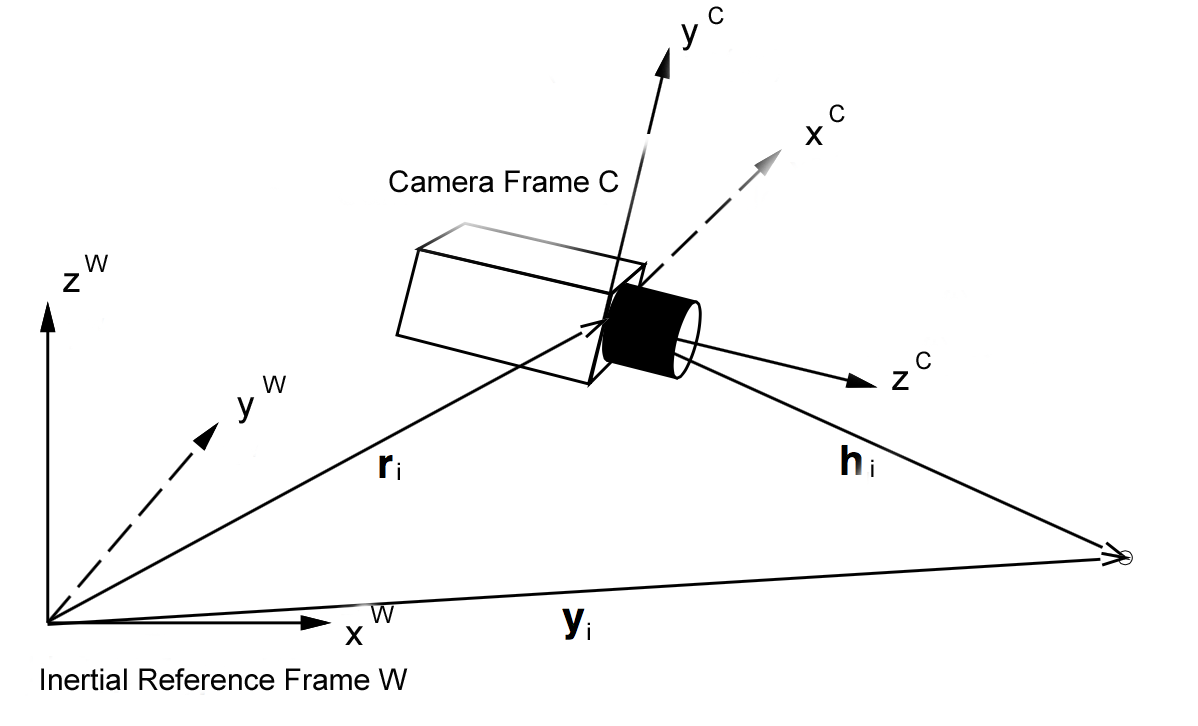
\includegraphics[width=0.8\linewidth,height=6cm]{Figures/frames.png}
\caption{Graphical representation of the appropriate reference frames. Adapted from~\cite{dav2007}}
\label{fig:frame}
\end{figure}
A quaternion, as previously mentioned, represents the camera's orientation. Quaternions are chosen as opposed to Euler angles to prevent the scenario where one degree of freedom is lost due to two of axes aligning. This scenario is more commonly referred to as a \textit{gimbal lock} and can cause a body to rotate unexpectedly between time steps. It should be noted that all quaternions represented in this paper are unit quaternions. This implies that the square root of the sum of all the squared elements is always equal to 1:
\begin{equation}
\textit{q}_{0,t}^2 + \textit{q}_{1,t}^2 + \textit{q}_{2,t}^2 + \textit{q}_{3,t}^2 = 1.
\end{equation}
When a robot's orientation changes, the process of computing the quaternions that causes this orientation change involves obtaining an angle-axis as well as a magnitude by which this axis is to be rotated. This process is described later in this chapter with reference to the state transition model probability.

Often, the modelling of dynamic systems require that additional parameters - apart from those describing the position and orientation of the robot - be included in the state vector. This is illustrated in Equation~\ref{eq:camvec}, where the linear velocity vector, $\textbf{v}^W$, forms the additional information required for system modelling. This is due to the equivalent control input, that is of such a nature that an intermediary state (namely the linear velocity) is required to describe the control input's effect on the actual position. 
%%%%%%%%%%%%%%%%%%%%%%%%%%%%%%%%%%%%%%%%%%%%%%%%%%%%%%%%%%%%%%%%%%%%%%%%%%

%%%%%%%%%%%%%%%%%%%%%%%%%%%%%%%%%%%%%%%%%%%%%%%%%%%%%%%%%%%%%%%%%%%%%%%%%%   
\subsubsection{Feature Representation}
The probabilistic map contains a 3D position of \textit{each} observed landmark as well as a corresponding uncertainty. The feature estimates $\textbf{{y}}_i$ - consists of $n$ landmarks - are described through three individual coordinates - $x$, $y$ and $z$ respectively:
\begin{equation}
\textbf{{y}}_n = (x_n\hspace{0.25cm}y_n\hspace{0.25cm}z_n)^T,
\end{equation}
where the subscript $n$ denotes a specific landmark.
%\textcolor{red}{With reference to the theory on image processing, it can be discussed that the depth of a given landmark (in this case the $z$-coordinate) cannot be immediately determined, but rather approximated via triangulation given the landmark is observed over a sequence of (minimally) two known camera positions. The $x$ and $y$ measurements however, can be immediately determined from the image plane.}
\newpage
%%%%%%%%%%%%%%%%%%%%%%%%%%%%%%%%%%%%%%%%%%%%%%%%%%%%%%%%%%%%%%%%%%%%%%%%%%
\subsubsection{Sensor Model: Camera} \label{sec:cam}
The sensor of the the robot is a single CMOS digital camera. The \textit{pinhole camera model} depicted in Figure~\ref{fig:pinhole} is used to provide a reasonable approximation for a projection of a 3D point in space. The pinhole model however, ignores the effects of distortions caused by lenses and finite apertures. The model can however be adapted to account for these assumptions and better approximate the distortion.

The pinhole camera model contains a two-dimensional plane, with the projections of the 3D point $(x_i\hspace{0.2cm} y_i\hspace{0.2cm}z_i)^T$. The process of representing a 3D coordinate in terms of a 2D coordinate $(u_i\hspace{0.2cm}v_i)^T$ is known as \textit{perspective projection}. The 2D plane is commonly referred to as the \textit{pinhole plane} which contains a infinitesimal hole at its centre - the \textit{pinhole}. The camera possess its own 3D coordinate system with coordinate axes $X_C$, $Y_C$ and $Z_C$ (also referred to as the camera's \textit{optical axis}). The pinhole is situated at the origin of this 3D coordinate system - this is also referred to as the \textit{optical centre}. The \textit{image plane} is located at a positive distance \textit{f} from the optical centre \textit{O}, parallel to the pinhole plane. This distance $f$ is referred to as the camera's \textit{focal length}.     
\begin{figure}[h]
\begin{center}
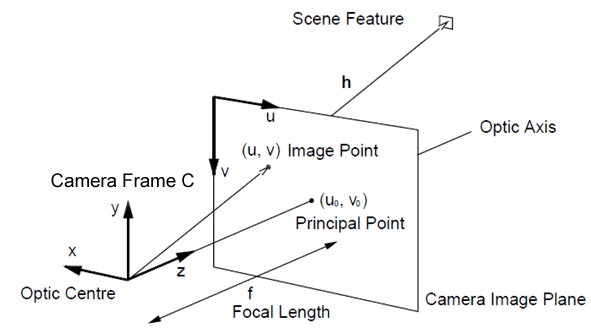
\includegraphics[width=0.9\textwidth, height=0.45\textwidth]{Figures/pinhole1.png}
\caption{Graphical representation of the pinhole camera model. The Figure shows the projection of a scene feature onto the camera image plain with respect to the camera's optic centre. The camera reference frame $C$ is defined at the optic centre of the camera. Adapted from~\cite{pinhole}.}
\label{fig:pinhole}
\end{center}
\end{figure}

The image of the camera represents a projection of a 3D point in space. Euclidean geometry requires complicated calculations to describe these projections. \textit{Projective geometry} offers an alternative representations of the geometry that is both simpler to implement. Projective geometry uses a system of coordinates called \textit{homogenous coordinates} and is able to represent transformations in a single matrix. The projection of an object $r$ is defined as homogenous if the same object is represented by $r = \lambda r$. The relationship between homogenous and Euclidean coordinates is shown according to a lecture presented by Stachnis~\cite{cyril}:
\begin{equation} 
\label{eq:fmmd1}
  \begin{pmatrix}
	u \\
	v \\
	w \\
  \end{pmatrix} =
    \begin{pmatrix}
	wx \\
	wy \\
	w \\
  \end{pmatrix} = 
    \begin{pmatrix}
	x \\
	y \\
	1 \\
  \end{pmatrix},
\end{equation}
where $x$ and $y$ are the Euclidean coordinates. 

The undistorted projection of a point in the image plane ($u_i$,$v_i$) is be derived using similar triangles and homogenous coordinates as presented in a thesis by Albrecht~\cite{master}:
\begin{equation} 
\label{eq:fmmd1}
\begin{split}
  \begin{pmatrix}
  u_i\\
  v_i\\
  1
  \end{pmatrix} =
  \begin{pmatrix}
  f & 0 & u_0\\
  0& f  & v_0\\
  0& 0 & 1 
  \end{pmatrix}
  \begin{pmatrix}
  \frac{u_i}{f} \\
  \frac{v_i}{f} \\
  1
  \end{pmatrix}
  =  \textbf{C}
  \begin{pmatrix}
  \frac{u_i}{f} \\
  \frac{v_i}{f} \\
  1
  \end{pmatrix}
 \textbf{C} &= 
 \begin{pmatrix}
  f & 0 & u_0\\
  0& f  & v_0\\
  0& 0 & 1 
 \end{pmatrix}
\end{split},
\end{equation}
where $\textbf{C}$ represents the camera's \textit{intrinsic matrix}, $u_0$ and $v_0$ represents the \textit{principal point} located at the image centre.

The camera's intrinsic matrix describes the parameters that are unique to a camera containing the principal point as well as the focal lengths. Once obtained, this matrix can be used to obtain the projections of any 3D point in an image plane, as well as an 3D approximation of a projected point.
As previously mentioned, the pinhole camera model ignores the effects of distortion that generally present in practical systems. To account for the errors that such an approximation may yield, it is proposed that the \textit{projected} coordinates ($u_i,v_i$) be warped with a \textit{radial distortion} as is done in~\cite{dav2007}, in order to obtain a coordinate ($u_d, v_d$), where the distortion has been accounted for. This radial distortion is mathematically shown as in a study presented by Swaminathan and Kayer~\cite{distort}:
\begin{equation} \label{eq:raddist}
\begin{split}
u_d - u_0 &= \frac{u-u_0}{\sqrt{1+2K_1r^2}} \\
v_d - v_0 &= \frac{v-v_0}{\sqrt{1+2K_1r^2}}, \\
r &= \sqrt{(u - u_0)^2+(v-v_0)^2},
\end{split}
\end{equation}
where $K_1$ and $r$ represent the radial distortion parameters. 
\newpage
%%%%%%%%%%%%%%%%%%%%%%%%%%%%%%%%%%%%%%%%%%%%%%%%%%%%%%%%%%%%%%%%%%%%%%%%%%
\subsubsection{Control Input Equivalent}\label{sec:imu}
%\textbf{Still reading up on some literature before properly defining this section}
The following concept describes the dynamics to the system as a result of external influences. Upon considering the original MonoSLAM approach, it is evident that there are no \textit{observable} control inputs. The approach presented in this paper though, aims to use measurements obtained through an IMU as an equivalent control input in order to derive a motion model that is potentially more accurate than the implementation of Davison et al.~\cite{dav2007}.

In most instances of robotics, it is essential to describe the dynamics involving a robot's movement. In the context of this paper, the robot (camera) is free to move as it pleases. %Evidently, these requests exert forces upon the robot which are unknown to the system. 
In the approach presented by Davison et al., a constant velocity model is assumed and at each time step, unknown linear and angular acceleration zero-mean, Gaussian processes are introduced that cause linear and angular velocity impulses. The model contains very little, if any information about the movement of the camera. It can be assumed that utilising additional information regarding the camera's movement will provide greater accuracy upon state estimation.

The IMU is comprised of inertial sensors, namely the accelerometer and gyroscope, that are mounted onto the camera. This allows the camera to be modelled as a rigid body upon which a kinematic estimation can be applied. The IMU directly measures the total acceleration $\textbf{f}_t$ as well as the total angular velocities $\boldsymbol{\psi}_t$ with respect to the camera's rigid body frame $C$. 

The measured acceleration and gyroscope measurements form the \textit{equivalent control vector} $\textbf{{u}}_t$ that describes, at each time step, the external forces exerted on the system with noise. The control vector equivalent is adapted as follows:

\begin{equation}
\textbf{u}_t = 
\begin{pmatrix}
\textbf{f}_t \\
\boldsymbol{\psi}_t
\end{pmatrix} =
\begin{pmatrix}
f_{x,t}&
f_{y,t}&
f_{z,t}&
\psi_{x,t}&
\psi_{y,t}&
\psi_{z,t}
\end{pmatrix}^T.
\end{equation}

Because the IMU measures the actual movements through sensors, namely an accelerometer and a gyroscope, the process noise is embedded within these measurements. Moreover, the uncertainty regarding the state transition model probability, namely the process noise, is all incorporated within the noise measurements of the IMU. This noise can be modelled as a zero mean, Gaussian RV's $\textbf{w}_t$ with a corresponding covariance matrix $\textbf{R}_w$. Because changes in orientation incorporates additional uncertainty to the system, this covariance matrix is required to be updated at each time step. The system noise can be then be mathematically described as follows:
 
\begin{equation} \label{eq:pertn}
\textbf{w}_t =
\begin{pmatrix} 
 \textbf{n}_{\textbf{a},t} \\
 \textbf{n}_{{\omega},t}
\end{pmatrix}
= \begin{pmatrix}\hspace{0.1cm}n_{\ddot{x}_{t}}\hspace{0.25cm}n_{\ddot{y}_{t}}\hspace{0.25cm}n_{\ddot{z}_{t}}\hspace{0.25cm}n_{{\omega}_{x,t}}\hspace{0.25cm}n_{{\omega}_{y,t}}\hspace{0.25cm}n_{{\omega}_{z,t}}\hspace{0.1cm}
\end{pmatrix}^T,
\end{equation}
with the aforementioned noise model is assumed to be a Gaussian random variable for each of the above elements.  

Furthermore the covariance matrix corresponding to the process noise is defined as follows:

\begin{equation}\label{eq:proR}
\textbf{R}_w =  
\begin{pmatrix}
n_{a_x,t}& 0 & 0 & 0 & 0 & 0 \\
0& n_{a_y,t} & 0 & 0 & 0 & 0 \\
0& 0 & n_{a_z,t} & 0 & 0 & 0 \\
0& 0 & 0 & n_{\psi_{x},t} & 0 & 0 \\
0& 0 & 0 & 0 & n_{\psi_{y},t} & 0 \\
0& 0 & 0 & 0 & 0 & n_{\psi_{z},t} \\
\end{pmatrix} ^2.
\end{equation}

The Kinematic estimator however, requires that the linear portion of the total acceleration $\textbf{f}_t$ be obtained from the IMU measurement. It is known that the total acceleration measured by the IMU's accelerometer is adapted from a study presented by Servent et. al~\cite{IMU}:

\begin{equation}\label{eq:acc}
\textbf{f}_t = \textbf{\text{R}}^{CW}(\textbf{a}^C_t + \textbf{g}),
\end{equation}
with $\textbf{a}_t$ is the linear acceleration vector with respect to the cameras reference frame $C$, $\textbf{g}$ is the gravity vector and $\textbf{\text R}^{CW}$ is the rotation matrix that transforms the camera's body coordinate frame $C$, into the inertial reference frame $W$.\\
The rotation matrix is defined according to a tutorial presented by Davison~\cite{models}:
\begin{equation}
\textbf{R}^{CW} = 
\begin{pmatrix}
q_{0,t}^2+q_{1,t}^2-q_{2,t}^2-q_{3,t}^2 & 2(q_{1,t}q_{2,t}-q_{0,t}q_{3,t}) & 2(q_{1,t}q_{3,t}-q_{0,t}q_{2,t}) \\ 
2(q_{1,t}q_{2,t} +q_{0,t}q_{3,t}) & q_{0,t}^2-q_{1,t}^2-q_{2,t}^2-q_{3,t}^2 & 2(q_{2,t}q_{3,t}-q_{0,t}q_{1,t}) \\ 
2(q_{1,t}q_{3,t}-q_{0,t}q_{2,t}) & 2(q_{2,t}q_{3,t}+q_{0,t}q_{1,t}) & q_{0,t}^2-q_{1,t}^2-q_{2,t}^2+q_{3,t}^2 \\ 
\end{pmatrix}.
\end{equation}

The linear acceleration is a processed measurement. Rearranging Equation~\ref{eq:acc}:
\begin{equation}
\textbf{a}_t = \textbf{R}^{WC}\textbf{f}_t - \textbf{g},
\label{eq:lina}
\end{equation}

where $\textbf{R}^{WC}$ is the inverse of the rotation matrix $\textbf{R}^{CW}$ and the inverse of a rotation matrix is its transpose:
\begin{equation}
\textbf{R}^{WC}=(\textbf{R}^{CW})^{-1}=  (\textbf{R}^{CW})^T.
\end{equation}

The rotation in Equation~\ref{eq:lina} presents an uncertainty that cannot be modelled as the additive noise defined in Equation~\ref{eq:pertn}. Incorporating this uncertainty is discussed in Chapter~\ref{sec:covup}.
%with the perturbation levels $n_{w,t}$ as defined in equation~\ref{eq:pertn}.
%%%%%%%%%%%%%%%%%%%%%%%%%%%%%%%%%%%%%%%%%%%%%%%%%%%%%%%%%%%%%%%%%%%%%%%%%%
\newpage
\subsection{Control Update Step}
With reference to the probabilistic form of the solution to the SLAM problem, the control update step requires a description in terms of a belief distribution. The description of the aforementioned belief, in terms of the probability distribution on the state transitions, is described in step 1 of Table~\ref{tab:BF} and repeated for convenience :
\begin{equation}
\overline {bel}(\textbf{x}_t) = \int p(\textbf{x}_t\hspace{0.1cm}|\hspace{0.1cm}\textbf{u}_{t},\hspace{0.1cm}\textbf{x}_{t-1})bel(\textbf{x}_{t-1})\hspace{0.1cm}d\textbf{x}_{t-1} ,
\end{equation}
The state transition model however, assumes the form of a Markov process, yielding that the current state $\textbf{{x}}_{t}$ is only dependent upon the state immediately preceding it - $\textbf{{x}}_{t-1}$ - as well as the input control $\textbf{{u}}_t$. Additionally, the uncertainty regarding the state transition model is independent of the uncertainty regarding both the observation model. This allows an implementation of the Bayes filter to be used, more specifically the EKF. This section presents the necessary steps to incorporate the control update of the EKF. 
%%%%%%%%%%%%%%%%%%%%%%%%%%%%%%%%%%%%%%%%%%%%%%%%%%%%%%%%%%%%%%%%%%%%%%%%%%
\begin{figure}[h]%{0.5\textwidth}
\centering
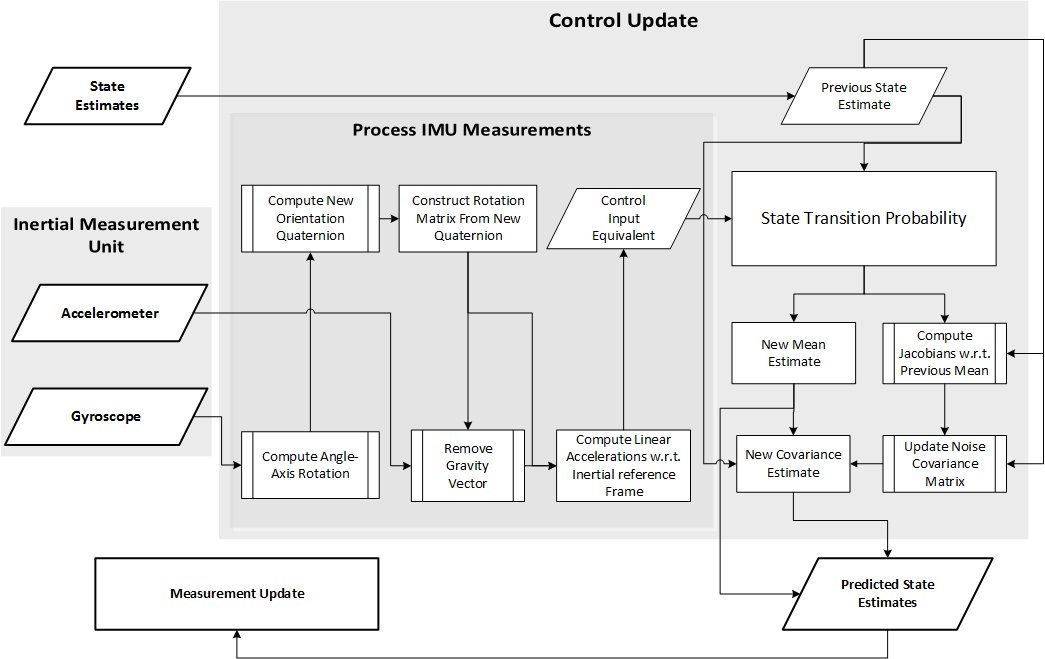
\includegraphics[width=\linewidth,height=0.78\textwidth]{Figures/Control_Update.png}
\caption{A detailed functional diagram of the control update step of the EKF. The greyed blocks depict functional subsystems}
\label{fig:contrup}
\end{figure}
%%%%%%%%%%%%%%%%%%%%%%%%%%%%%%%%%%%%%%%%%%%%%%%%%%%%%%%%%%%%%%%%%%%%%%%%%%
\subsubsection{State Transition Probability Model} 
The description of the aforementioned state transition probability model can then, in terms of the probability distribution on the state transitions, take the following form:
\begin{equation}
\begin{split}
p(\textbf{{x}}_t\hspace{0.15cm}|\hspace{0.15cm}\textbf{x}_{t-1}, \textbf{u}_t)&=\cfrac{1}{\sqrt{|2\pi\textbf{R}_w|}}\hspace{0.1cm}\text{exp}\hspace{0.1cm}\bigg\{ \frac{1}{2}\big[\textbf{{x}}_t-g(\textbf{u}_t, \hspace{0.1cm}\boldsymbol{\mu}_{t-1}) - \textbf{G}_t^{\textbf{x}_{t-1}}(\textbf{x}_{t-1} - \boldsymbol{\mu}_{t-1})\big]^T\\
&\textbf{R}^{-1}_w\big[\textbf{{x}}_t-g(\textbf{u}_t, \hspace{0.1cm}\boldsymbol{\mu}_{t-1}) - \textbf{G}_t^{\textbf{x}_{t-1}}(\textbf{x}_{t-1} - \boldsymbol{\mu}_{t-1})\big]\bigg \}
\end{split},
\end{equation} 
where $\textbf{G}_t^{\textbf{x}_{t-1}}$ represents the Jacobian of the state transition motion and $\textbf{R}_w$ is the process noise.

With reference to Chapter~\ref{sec:EKF}, the EKF requires a state transition probability model in order to obtain the mean estimate $ \boldsymbol{\bar \mu}_t$, of  current state of the system. In short, the state transition probability model describes the transition from the previous state to the following state with regard to the robot�s kinematic motion as well as the control inputs. In order to derive the state transition model for the system at hand, it is vital that certain characteristics of the system be understood. Firstly, the robot system - from here on in to be referred to as the \textbf{camera} - is comprised of a monocular camera and an attached IMU package. Secondly, the camera is to be considered as a six degree of freedom (DOF) rigid body. Briefly the six DOF describe the camera's three \textit{translational} and three \textit{rotational} degrees of freedom. 

We therefore set out to define a kinematic estimation based state transition probability model - using Newton's laws of motion - to describe the camera's movement through the environment as a result of initially unknown, external inputs to the system. Lastly, embedded within the motion model should be the impacts of uncertainty through both internal and external factors (noise).

A derivation for the suitable motion model will be obtained before a first order Taylor approximation is obtained as required by the EKF. recall the states and control inputs (equivalents):

\begin{equation}
\begin{split}
\textbf{x}_t &=
\begin{pmatrix}
\hspace{0.1cm}\textbf{r}_t^{W}\hspace{0.1cm}\textbf{q}_t^{WC}\hspace{0.1cm}\textbf{v}_t^{W}
\end{pmatrix}^T\\ 
%&=\begin{pmatrix}
%\textit{x}_{t}\hspace{0.25cm}\textit{y}_{t}\hspace{0.25cm}\textit{z}_{t}\hspace{0.25cm}\textit{q}_{0,t}\hspace{0.25cm}\textit{q}_{1,t}\hspace{0.25cm}\textit{q}_{2,t}\hspace{0.25cm}\textit{q}_{3,t}\hspace{0.25cm}\textit{\.{x}}_{t}\hspace{0.25cm}\textit{\.{y}}_{t}\hspace{0.25cm}\textit{\.{z}}_{t} 
%\end{pmatrix}^T\\
\textbf{u}_t
&=\begin{pmatrix}
\hspace{0.1cm}\textbf{f}_t^C\hspace{0.1cm}\boldsymbol{\psi}_t^C
\end{pmatrix}^T\\
%&=\begin{pmatrix}
%\hspace{0.1cm}\ddot{x}_{t}\hspace{0.25cm}\ddot{y}_{t}\hspace{0.25cm}\ddot{z}_{t}\hspace{0.25cm}{\omega}_{x,t}\hspace{0.25cm}{\omega}_{y,t}\hspace{0.25cm}{\omega}_{z,t}\hspace{0.1cm}
%\end{pmatrix}^T\\
\end{split}.
\end{equation}
\\\\
Considering that the EKF is a recursive, numerical evaluation, it is necessary to convert the \textit{continuous} linear differential equations that describe the state transition model into a discrete counterpart. Various methods of discretisation exist, though this specific implementation makes use of the forward difference (Euler�s) method as the sampling period is assumed to be small enough. This method \textit{approximates} the derivative for a state for a sampling period $\Delta T$ as follows:  
\begin{equation}
\begin{split}
\textbf{\.{x}}_{t-1} &= \lim_{\Delta T\to 0}{\frac{\textbf{x}_{t}-\textbf{x}_{t-1}}{\Delta T}} 		 \\										 \textbf{x}_{t} &\approx \textbf{\.{x}}_{t-1}\Delta T + \textbf{x}_{t-1}
\end{split}.
\end{equation}  
Newton's second law of motion, describing the relationship between a body's mass and its acceleration, is used to derive the linear motion model after which the aforementioned method of discretisation is applied to obtain the discrete motion model. A full derivation of the linear state transition model is shown in Appendix~\ref{App:Concepts}.

The non-linear state transition function of the kinematic estimator $\textbf{g}(\textbf{u}_{t},\textbf{x}_{t-1})$ is defined at the current time $t$, is dependent on both the current control input equivalents $\textbf{u}_t$ as well as the actual states $\textbf{x}_{t-1}$. The non-linear behaviour is a result of the change in orientation of the camera. The state transition function is defined and adapted from a tutorial presented by Davison~\cite{models}:
\begin{equation} \label{eq:trmod}
\begin{split}
\textbf{g}(\textbf{u}_{t},\textbf{x}_{t-1}) =
	\begin{pmatrix}
		\textbf{r}_t^{W}\\
		\textbf{q}_t^{WC}\\
		\textbf{v}_t^{W} \\
	\end{pmatrix} &= 
	\begin{pmatrix}
		\textbf{r}_{t}^{W}+\textbf{v}_{t-1}^W\Delta T\\
		\textbf{q}_{t-1}^{WC} \otimes \text{quat}\big(\boldsymbol{\omega}_t^C\Delta T\big) \\
		\textbf{v}_t^{W} + \textbf{a}_{t-1}^W \Delta T \\
	\end{pmatrix} \\
&= \begin{pmatrix}
	 \textbf{r}_{t-1}^{W}+\textbf{v}_{t-1}^W\Delta T\\
	 \textbf{q}_{t-1}^{WC} \otimes \text{quat}\big(\boldsymbol{\omega}_t^C\Delta T\big) \\
	 \textbf{v}_t^{W} + \textbf{R}_{t-1}^{CW}\big(\textbf{a}_{t-1}^C \Delta T\big) \\
\end{pmatrix} \\
\end{split},
\end{equation}
where $\text{quat}\big(\boldsymbol{\omega}_t^C\Delta T\big)$ denotes the process of obtaining the quaternions of the rotation $\boldsymbol{\omega}_t^C\Delta T$ and $\Delta T$ is defined as the sample period between the previous time $t-1$ and $t$.  

The angular velocities $\boldsymbol{\omega}_t^C$ and the linear accelerations $\textbf{a}_{t-1}^W$ are measured from the control input equivalent $\textbf{u}_t$ and the position $\textbf{r}^{W}_{t-1}$, linear velocity $\textbf{v}^{W}_{t-1}$ and the orientation quaternion $\textbf{q}_{t-1}^{WC}$ - and subsequently the rotation matrix $ \textbf{R}_{t-1}^{CW}$ - are obtained from the previous state vector.\\

In order to compute the quaternions, the rate at which the camera's rotational degrees of freedom are changing is required. The control input equivalent, measure exactly this quantity from the gyroscope - the angular velocity. The angular velocity is subsequently numerically integrated in order to obtain the angular position $\boldsymbol{\theta}_t$, before the quaternion is taken thereof. As previously mentioned, an angle-axis as well as a magnitude by which this axis is to be rotated is required to compute a quaternion. The angle-axis $\boldsymbol{\gamma}_t$ is defined at a particular time instance $t$ according to a tutorial presented by Davidson~\cite{models}:
\begin{equation} \label{eq:axis}
\begin{split}
\boldsymbol{\gamma}_t &= \begin{pmatrix}
\boldsymbol{\theta}_t, {\norm{\boldsymbol{\theta}_t}} 
\end{pmatrix} =
\begin{pmatrix}
\begin{pmatrix}
\theta_{x,t} \\
\theta_{y,t} \\
\theta_{z,t} 
\end{pmatrix}, \norm{\boldsymbol{\omega}_t^C \Delta T} 
\end{pmatrix} = 
\begin{pmatrix}
\begin{pmatrix}
\frac{\omega_{t,X}^C \Delta T}{\norm{\boldsymbol{\omega}_t^C \Delta T}} \\
\frac{\omega_{t,Y}^C \Delta T}{\norm{\boldsymbol{\omega}_t^C \Delta T}} \\
\frac{\omega_{t,Z}^C \Delta T}{\norm{\boldsymbol{\omega}_t^C \Delta T}}  
\end{pmatrix}, \norm{\boldsymbol{\omega}_t^C \Delta T} 
\end{pmatrix}
\end{split},
\end{equation}

where $\omega_{t,\beta}$, $\beta \in \{X, Y, Z\}$ denotes the angular velocity about each respective coordinate axis. The result in Equation~\ref{eq:axis} is then represented as a unit quaternion denoting the same rotation~\cite{models}:

\begin{equation} \label{eq:quat} 
\textbf{q} = \bigg(\cos \frac{\alpha}{2} \hspace{0.4cm} \frac{\theta_x}{\norm{\boldsymbol{\theta}}}\sin\frac{\alpha}{2} \hspace{0.4cm} \frac{\theta_y}{\norm{\boldsymbol{\theta}}}\sin\frac{\alpha}{2} \hspace{0.4cm} \frac{\theta_z}{\norm{\boldsymbol{\theta}}}\sin\frac{\alpha}{2} \bigg)^T.
\end{equation}

A quaternion multiplication between the quaternion $\textbf{q}^{WC}_{t-1}$ and the angle-axis rotation quaternion in Equation~\ref{eq:quat} represents the product of the two rotation matrices each quaternion represents. This quaternion multiplication is denoted by the $\otimes$ operator in equation~\ref{eq:trmod} is formally defined according to a tutorial presented by Davidson~\cite{models}:

\begin{equation}
\begin{split}
\textbf{q}^{WC}_t 	&= \textbf{q}_{t-1}^{WC} \otimes \text{quat}(\boldsymbol{\omega}^C_t\Delta T) \\ 
		            	&=\textbf{q}_1 \times \textbf{q}_2 \\
				&=\begin{pmatrix}
				q_{1,0}q_{2,0} - (q_{1,2}q_{2,1} + q_{1,2} q_{2,2} + q_{1,3}q_{2,3})\\
				q_{1,0}\begin{pmatrix}
				q_{2,1}\\
				q_{2,2}\\
				q_{2,3}
				q_{2,0}\end{pmatrix} +
				\begin{pmatrix}
				q_{1,1}\\
				q_{1,2}\\
				q_{1,3}
				\end{pmatrix}+
				\begin{pmatrix}
				q_{1,2}q_{2,3} - q_{2,2}q_{1,3}\\
				q_{1,3}q_{2,1} - q_{2,3}q_{1,1}\\
				q_{1,1}q_{2,2} - q_{2,1}q_{1,2}\\
				\end{pmatrix}
\end{pmatrix}
\end{split}.
\end{equation}
This completes the steps necessary to implement the state transition probability model. 
%%%%%%%%%%%%%%%%%%%%%%%%%%%%%%%%%%%%%%%%%%%%%%%%%%%%%%%%%%%%%%%%%%%%%%%%%%
\subsubsection{Mean Estimate}\label{sec:kinest}
The control update uses the previously defined state transition probability function to obtain a state estimate $\boldsymbol{\bar \mu}_t$ at the current time instance. This procedure is shown in Step 1 of Table~\ref{tab:EKF}. Recalling Equation~\ref{eq:trmod}, the state transition function is dependent on both the current equivalent control inputs as well as the actual states to obtain a suitable state estimate:

\begin{equation} \label{eq:trmod1}
\begin{split}
\textbf{g}(\textbf{u}_{t},\boldsymbol{\mu}_{t-1}) 
&= \begin{pmatrix}
	 \textbf{r}_{t}^{W}+\textbf{v}_{t-1}^W\Delta T\\
	 \textbf{q}_{t-1}^{WC} \otimes \text{quat}\big(\boldsymbol{\omega}_t^C\Delta T\big) \\
	 \textbf{v}_t^{W} + \textbf{R}_{t-1}^{CW}\big(\textbf{v}_{t-1}^C \Delta T\big) \\
\end{pmatrix} \\
\end{split}.
\end{equation}

It is worthwhile to note that the equivalent control inputs (which are the measurements from the IMU) incorporates zero-mean process noise but is modelled accordingly in the covariance update in Chapter~\ref{sec:covup}.
%%%%%%%%%%%%%%%%%%%%%%%%%%%%%%%%%%%%%%%%%%%%%%%%%%%%%%%%%%%%%%%%%%%%%%%%%%
\subsubsection{Covariance Update}\label{sec:covup}
Before the control update can be concluded, the covariance matrix $\boldsymbol{\bar \Sigma_t}$, corresponding to the previously determined mean vector $\boldsymbol{\bar \mu_t}$ is required to be updated as a result of the linearisation process undertaken by the EKF. This procedure is denoted in Step 2 of Table~\ref{tab:EKF}. It can be noticed that the previously described Jacobian matrix of $\textbf{g}(\textbf{u}_{t},\textbf{x}_{t-1})$ evaluated at the predicted mean $\boldsymbol{\mu}_{t-1} $ is thus required to realise this procedure. The Jacobian matrix $\textbf{G}_t^{\textbf{x}_{t-1}}$ can be mathematically defined using Equation~\ref{eq:par}:

\begin{equation} \label{eq:jacG}
\textbf{G}_t^{\textbf{x}_{t-1}} = \frac{\partial \textbf{g}(\textbf{u}_{t},\textbf{x}_{t-1})}{\partial \textbf{x}_{t-1}}\bigg|_{\textbf{x}_{t-1}= \boldsymbol{\mu}_{t-1}} 
=\begin{pmatrix}
\frac{\partial \textbf{r}^W_t}{\partial \textbf{r}^W_{t-1}} & \boldsymbol{0} & \frac{\partial \textbf{r}^W_{t}}{\partial \textbf{v}^W_{t-1}}\\
\boldsymbol{0} & \frac{\partial \textbf{q}^{WC}_{t}}{\partial \textbf{q}^{WC}_{t-1}} & \boldsymbol{0}  \\
\boldsymbol{0} & \boldsymbol{0} & \frac{\partial \textbf{v}^W_{t}}{\partial \textbf{v}^W_{t-1}}  \\
\end{pmatrix}, 
\end{equation}   
with the non-zero elements of the Jacobian further trivially defined as follows (and according to the model defined in Equation~\ref{eq:trmod}),

\begin{equation}
\frac{\partial \textbf{r}^W_t}{\partial \textbf{r}^W_{t-1}} = \frac{\partial \textbf{v}^W_{t}}{\partial \textbf{v}^W_{t-1}} =
\begin{pmatrix} \label{eq:iden}
1 & 0 & 0\\
0 & 1 & 0\\
0 & 0 & 1\\
\end{pmatrix} = \textbf{I},
\end{equation}
and

\begin{equation} \label{eq:tiden}
\frac{\partial \textbf{r}^W_{t}}{\partial \textbf{v}^W_{t-1}} = 
\Delta T\begin{pmatrix}
1 & 0 & 0\\
0 & 1 & 0\\
0 & 0 & 1\\
\end{pmatrix} = \Delta T\hspace{0.2cm}\textbf{I}.
\end{equation}
The specially defined Jacobian with a partial derivative that is taken with respect to a quaternion however, requires a more intricate solution. The process of defining a new quaternion from the measured angular velocity $\boldsymbol{\omega}_t^C$ - is shown in Equation~\ref{eq:quat}%as denoted in Equation~\ref{eq:trmod} can be more formally defined from a tutorial a tutorial presented by Davison~\cite{models}:

\begin{equation}
%\begin{split}
\textbf{q}_t^C = \text{quat}(\boldsymbol{\omega}^C_t \Delta T) 
%&= \begin{pmatrix}\\
%\end{pmatrix}
%\end{split}.
\end{equation}
Hereafter, the final non zero element of the Jacobian can be defined in terms of the aforementioned new quaternion: 

\begin{equation}
\frac{\partial \textbf{q}^{WC}_{t}}{\partial \textbf{q}^{WC}_{t-1}} = 
\begin{pmatrix}
 q^C_{1,t}&-q^C_{2,t} & -q^C_{3,t} & -q^C_{4,t}\\
 q^C_{2,t}&  q^C_{1,t} & -q^C_{4,t} &  q^C_{3,t}\\
 q^C_{3,t}&  q^C_{4,t} &  q^C_{1,t} & -q^C_{2,t}\\
 q^C_{4,t}& -q^C_{3,t} &  q^C_{2,t} &  q^C_{1,t} \\
\end{pmatrix}.
\end{equation}
%\textcolor{blue}{TODO: show noise uncertainty that i used in practical application}
In order to complete the covariance update, the process noise covariance is still required to be updated. The additive process noise is captured by the IMU measurements and modelled as a zero-mean Gaussian process. The noise covariance $\textbf{R}_w$ however, incorporates additional uncertainty regarding the processing of the linear acceleration $\textbf{a}_t$ from the total acceleration $\textbf{f}_t$ :

\begin{equation}
\label{eq:Rt}
\begin{split}
\textbf{R}_{w,t} &= 
\frac{\partial \textbf{g}(\textbf{u}_{t},\boldsymbol{\mu}_{t-1})}{\partial \textbf{w}_{t-1}} 
\textbf{R}_{w_{t-1}}
\frac{\partial \textbf{g}(\textbf{u}_t,\boldsymbol{\mu}_{t-1})}{\partial \textbf{w}_{t-1}}^T \\  
&= \begin{pmatrix}
\textbf{I} \Delta T & \boldsymbol{0} \\
\boldsymbol{0} &  \frac{\partial \textbf{q}^{WC}_{t}}{\partial \boldsymbol{\omega}^{C}_{t-1}} \\
\end{pmatrix} \textbf{R}_{w_{t-1}}
 \begin{pmatrix}
\textbf{I} \Delta T & \boldsymbol{0} \\
\boldsymbol{0} &  \frac{\partial \textbf{q}^{WC}_{t}}{\partial \boldsymbol{\omega}^{C}_{t-1}} \\
\end{pmatrix}^T
\end{split},
\end{equation}

where the Jacobian element $\frac{\partial \textbf{q}^{WC}_{t}}{\partial \boldsymbol{\omega}^{C}_{t-1}}$ incorporates an uncertainty due to rotations.

This completes the deviations necessary to fully incorporate the control update step of the EKF.
%%%%%%%%%%%%%%%%%%%%%%%%%%%%%%%%%%%%%%%%%%%%%%%%%%%%%%%%%%%%%%%%%%%%%%%%%%
\newpage
\subsection{Measurement Update}
With reference again to the probabilistic form of the solution to the SLAM problem, the measurement step too, requires a description in terms of a belief distribution. This belief, in terms of the probability distribution on the measurements, is described in step 2 of Table~\ref{tab:BF} and repeated for convenience :
\begin{equation}\label{eq:belpred}
 {bel}(\textbf{x}_t) = \eta p(\textbf{z}_t\hspace{0.1cm}|\hspace{0.1cm}\textbf{x}_{t})\overline {bel}(\textbf{x}_t)
\end{equation}
The correction step seeks to incorporate an actual measurement $\textbf{{z}}_t$ into the state estimate through incorporating the previously mentioned weighted mean upon updating the mean prediction and covariance prediction estimates. The measurement update of the EKF in this project is identical to the measurement update of the existing MonoSLAM implementation~\cite{dav2007}. A functional diagram of the measurement update is shown in Figure~\ref{fig:measup}.

The focus of this project is to incorporate additional information to improve the motion estimation of a robot. The literature study showed that the utilisation of additional measurement sensor is both expensive and difficult to integrate with the existing implementation (this is stated in Chapter~\ref{sec:into2}). It is also expected that improvements to the existing measurement update of MonoSLAM will not improve the state estimates significantly. As a result, a decision is made to incorporate the existing measurement update directly as presented in the study by Davidson et al.~\cite{dav2007}
\begin{figure}[h]%{0.5\textwidth}
\centering
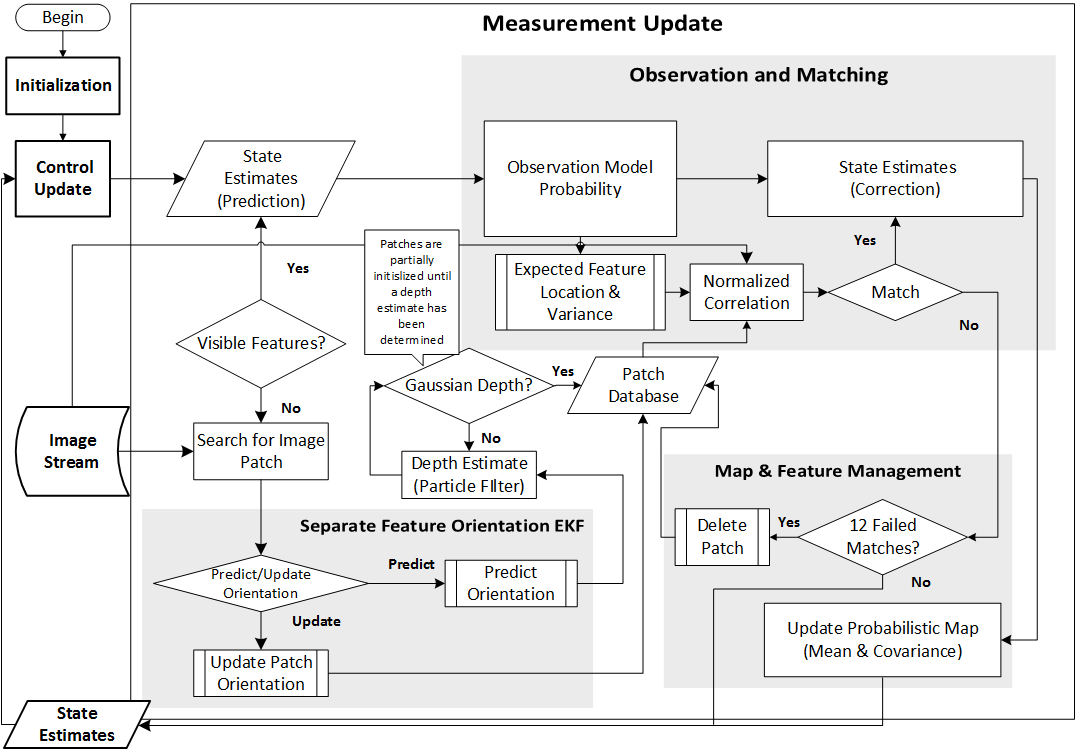
\includegraphics[width=\linewidth,height=0.78\textwidth]{Figures/Mes_alt.png}
\caption{A detailed functional diagram of the measurement update step of the EKF. The greyed blocks depict functional subsystems}
\label{fig:measup}
\end{figure}
%%%%%%%%%%%%%%%%%%%%%%%%%%%%%%%%%%%%%%%%%%%%%%%%%%%%%%%%%%%%%%%%%%%%%%%%%%
\subsubsection{General Overview}
This section seeks to provide an informative yet concise overview of the measurement update that is implemented in this project. Although no alterations were made to this subsection of the project, the reader requires an understanding of the basic operations that are fundamental to the realisation of this project.       

This particular vision based approach aims to use salient image \textit{patches} as long term landmarks as presented in \cite{dav2007,actvis}. These aforementioned patches are typically 11 $\times$ 11 pixels and are obtained through the image detection operator of Shi and Tomasi~\cite{shitom} from raw monochrome images. The goal is to repeatedly re-identify these image template patches over time after considerable camera movements. Invariably, basic 2D template matching algorithms are of little use, considering that any particular movements of the camera (even minimal) can severely alter the shape of a saved template patch. As a result, MonoSLAM assumes that each patch lies on a locally planar surface and that the surface normal is parallel to the vector from the feature to the camera. Once the depth of a patch has been determined - this is done through a small particle filter - the patch is stored to be used as a long term landmark. MonoSLAM stores these patches to provide a template for matching against a newly obtained 2D image at a later stage. A warped version of the patch is projected back into the image upon matching to account for the potential error provided by the orientation assumption. Because the appearance of the patches are never updated and remain in memory, long term localisation is possible. The orientation of the features however, are updated using a separate EKF - this is depicted in Figure~\ref{fig:measup}.

%The measurement model is able to obtain a search area around which the system expects an initialised feature to be. 
The measurement model can provide a prediction regarding a feature's coordinate in the current image based on the prior movement estimates of the camera. The \textit{innovation matrix} describes the 2D Gaussian uncertainty regarding this position, providing an elliptical region around the predicted coordinate. A normalised cross-correlation is conducted within this search region seeking to match an initialised feature within the current image.  

The EKF measurement update is concluded through the steps shown in Table~\ref{tab:EKF} after the probabilistic map is updated. An additional process outside of the operation of the EKF is required to achieve this process. This process is described in Chapter~\ref{sec:mapman}.   
%With regard to the management of the probabilistic map, it remains essential to the SLAM algorithm that decisions regarding the identification and deletion of landmarks be accurate and efficient. MonoSLAM's map-maintenance criterion demands that 12 reliable ``good" features be visible within the camera's field of view in order to maintain accurate localisation. A good feature implies that a feature remains visible within the camera's field of view. A new feature is initialised using the image operator of Shi and Tomasi~\cite{shitom} upon a box of pixels (80 $\times$ 60 pixels) placed within an image. This box position is chosen at random with the constraints that it shouldn't overlap with any existing features and that it remains in the camera's field of view. If a visible feature is unsuccessfully matched more than 50\% of the time, the landmark is deleted. It must be stressed that the aforementioned methods regarding vision based MonoSLAM measurements and map-management are described and implemented in this project exactly as they are in ~\cite{dav2007}. 

%%%%%%%%%%%%%%%%%%%%%%%%%%%%%%%%%%%%%%%%%%%%%%%%%%%%%%%%%%%%%%%%%%%%%%%%%%
\subsubsection{Probabilistic Map Management}\label{sec:mapman}
In order to realise the solution to the SLAM problem, the measurement update of a system requires an additional process - namely \textit{data association} or \textit{map management}. The criteria regarding this map management typically differs according to the application, but the general idea is that the map continuously deletes and adds features accordingly.

In MonoSLAM, the criteria of this map management is determined via a trade off between two factors: number of features in a camera's field of view and the computation expense. MonoSLAM seeks to, at every given time instance, keep the number of features visible within the camera's field of view close to a predetermined value. This value is 12 by default, but can be adjusted according to the computing power available. 

The detection operator of Shi and Tomasi~\cite{shitom} seeks to initialise new features if the number of features visible in the cameras field of view drops below the predetermined value. These features are initialised if a prediction based on the camera's movement suggests that the feature will remain in the camera's field of view in the subsequent frames. Additionally, a feature is deleted from the map if it fails 50\% of successive detection and matching attempts.  
%%%%%%%%%%%%%%%%%%%%%%%%%%%%%%%%%%%%%%%%%%%%%%%%%%%%%%%%%%%%%%%%%%%%%%%%%%
%%%%%%%%%%%%%%%%%%%%%%%%%%%%%%%%%%%%%%%%%%%%%%%%%%%%%%%%%%%%%%%%%%%%%%%%%%
%\subsubsection{System Update
%%%%%%%%%%%%%%%%%%%%%%%%%%%%%%%%%%%%%%%%%%%%%%%%%%%%%%%%%%%%%%%%%%%%%%%%%%
\newpage
%%%%%%%%%%%%%%%%%%%%%%%%%%%%%%%%%%%%%%%%%%%%%%%%%%%%%%%%%%%%%%%%%%%%%%%%%%
\section{Implementation}\label{sec:impl}
\subsection{Introduction}
This Chapter sets out to discuss the hardware and software decisions that are made with respect to this project. Initially, the system requirements are presented and possible solutions are discussed. Thereafter, the individual hardware components used in this project are presented and motivated. This chapter also provides the  necessary configuration for each component to realise the system requirements. %Lastly, the core of this project, the kinematic estimator, is simulated and analysed as a possible alternative to the current velocity and angular velocity model. 
%%%%%%%%%%%%%%%%%%%%%%%%%%%%%%%%%%%%%%%%%%%%%%%%%%%%%%%%%%%%%%%%%%%%%%%%%%
\subsection{System Requirements}\label{sec:specs}
%%%%%%%%%%%%%%%%%%%%%%%%%%%%%%%%%%%%%%%%%%%%%%%%%%%%%%%%%%%%%%%%%%%%%%%%%%
The project objectives in Chapter~\ref{sec:into3} allow processing regarding the MonoSLAM implementation to be conducted on a personal computer (PC). In the original implementation of MonoSLAM, a 1.6 GHz Pentium M processor is used. Standard PC's however, provide no simple interface with external components that don't possess the peripheral ports present on the PC e.g. USB, Ethernet, Firewire and VGA. If indeed components can be connected via one of the aforementioned ports, a complicated procedure is often required if certain external components are required to communicate with one another through the PC.

The MonoSLAM implementation described in this project requires sensor measurements from a camera and motion measurements from an IMU. These components are also required to be synchronised. While cameras typically possess USB/Firewire/Ethernet ports allowing an interface with a PC, IMU's are typically IC's mounted on a PCB and contain no ports whatsoever. 

Wireless connectivity such as Bluetooth and Wifi provide an alternative for data communication. This wireless connectivity requires as both the PC and each sensor to possess an expensive integrated chip to enable this functionality and can also be difficult to implement. Micro-controllers however are cheap devices that allow a virtual interface to the PC for external hardware components. Micro-controllers are programmable devices and typically contain a range of digital and analogue input and output (I/O) ports. The programmable nature of these devices allow a certain degree of control regarding the design and functionality of the system. 

As a result, this project utilises a micro controller to provide the synchronisation between the camera and IMU as well as obtaining the data from the IMU and relaying it to the PC.  

%The primary sensor of the MonoSLAM implementation is a CMOS camera such as an IMU
An overview of the components required to realise the overall system as well as their interaction between one another is depicted in Figure~\ref{fig:sys}. It is evident that the system contains three hardware subsystems:
\begin{itemize}
\item Micro-controller.
\item Inertial measurement unit.
\item CMOS camera.
\end{itemize}

Each of of the subsystems require a unique setup configuration in order to represent a \textit{functional} unit of the whole system.   
%%%%%%%%%%%%%%%%%%%%%%%%%%%%%%%%%%%%%%%%%%%%%%%%%%%%%%%%%%%%%%%%%%%%%%%%%%%
\newpage
\subsubsection{Inertial Measurement Unit}
Chapter~\ref{sec:kinest} shows that inertial measurements are required in order to realise the implementation proposed in this project. The inertial measurements consists of 3 accelerometer and 3 gyroscope measurements. The combination of these sensors form a 6 \textit{degrees of freedom} (DOF) IMU. Accelerometers and gyroscopes can be analogue or digital devices that represent their measurements as either a voltage or a digital value respectively. This project seeks digital values that can be used by the PC to incorporate the measurements into the MonoSLAM algorithm.

A digital IMU with an accelerometer and gyroscope mounted on the same IC should ideally be purchased as there is time limit imposed on this project. Table~\ref{tab:imuspec} compares the necessary characteristics with a suitable IMU option, the SparkFun 6DOF IMU:
\begin{table}[H]
\caption{IMU necessary characteristics}
\centering
\begin{tabular}{|c|c|c|c|}
\hline
Characteristic & SparkFun 6DOF IMU & SparkFun 9DOF IMU & Required\\
\hline
\hline
\pbox{3cm}{Serial communication} & \pbox{3cm}{I2C/SPI (100 kHz \& 400 kHz)} & \pbox{3cm}{I2C/SPI (100 kHz \& 400 kHz)}& I2C (100 kHz) \\
\hline
\pbox{3cm}{Components} & \pbox{3cm}{Accelerometer, Gyroscope} &  \pbox{3cm}{Accelerometer, Gyroscope, Magnetometer} &  \pbox{3cm}{Accelerometer, Groscope}\\
\hline
\pbox{3cm}{Low pass filter (anti-aliasing)} & yes  & yes & yes  \\
\hline
\pbox{3cm}{Maximum data rate} & $3200$ Hz & $3200$ Hz  & 30 Hz \\
\hline
\hline
\textbf{Price} & R 489.99 & R620 &  $\leq$ R 500 \\
\hline
\end{tabular}
\label{tab:imuspec}
\end{table}%

The IMU cannot precisely sample measurements at the given system sampling period (30 Hz). The closest possible output data rate that exceeds the required system sampling period is 50 Hz. This however shouldn't limit the system functionality as the output data rate is greater than what is required. It should be noted that the IMU internal sampling rate is set to 3200 Hz for the accelerometer and 1000 Hz for the gyroscope - far more than the Nyqvist frequency. Additionally, the low pass filter is set to a bandwidth of 100 Hz to prevent aliasing.

%\begin{itemize}
%\item Communication with a master device (in this case a micro-controller).
%\item Suitable range that the sensors are capable of measuring.
%\item Noise on sensors.
%\item Communication speed.
%\item Low pass filter to prevent aliasing.
%\item Sample code.
%\end{itemize}
%
\begin{figure}[H]
\centering%\begin{center}
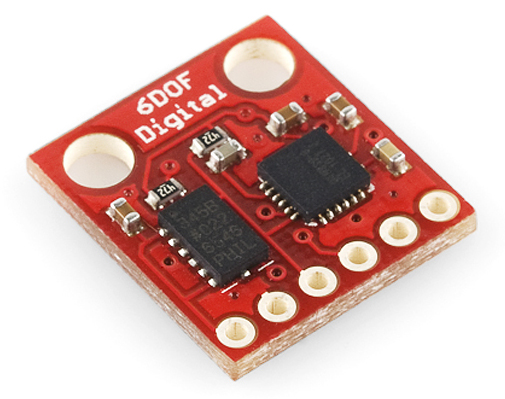
\includegraphics[keepaspectratio=true, scale = 1.4]{Figures/imu1.jpg}
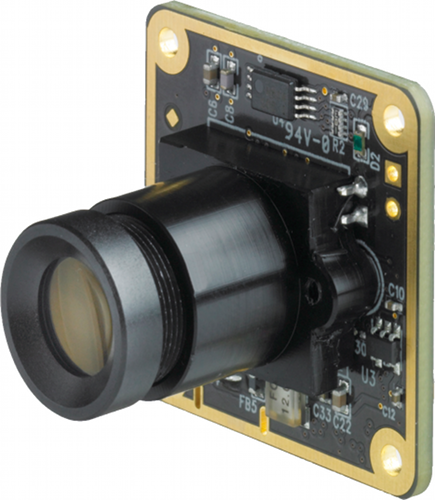
\includegraphics[keepaspectratio=true, scale = 0.275]{Figures/cam.png}
\caption{Left: SparkFun 6DOF IMU. Photo by SparkFun. Adapted from~\cite{create}. Right: The Imaging Source 22BUC03-ML CMOS board camera. Adapted from~\cite{imsrc}}
\label{fig:imu}
%\end{center}
\end{figure}
\newpage
The SparkFun 6 DOF IMU as depicted in Figure~\ref{fig:imu} provides the necessary characteristics for this project. This board is comprised of a ITG3200 MEMS 3-axis gyroscope~\cite{gyro} and a ADXL345 3-axis linear accelerometer~\cite{acc}. This component was chosen as it contains both the necessary sensors on the same chip while supporting I2C communication, an anti-alias filter, suitable range, sample code. 

Alternative products such as the 9DOF SparkFun IMU shown in Table~\ref{tab:imuspec} generally contain an additional 3 DOF while the required project specifications are identical or marginally better than that of the SparkFun 6DOF IMU. The additional 3 DOF provided by the magnetometer are assumed to be redundant and overlooked considering that these products are considerably more expensive than the chosen component. 

Finally, the IMU is configured in measurement mode with the following properties:
\begin{table}[h]
\caption{IMU configuration properties}
\centering
\begin{tabular}{|c|c|}
\hline
Parameter & Value \\
\hline\hline
Serial communication & I2C \\
\hline
Accelerometer range & $\pm4$g per second\\
\hline
Resolution & 10 bits \\
\hline
Gyroscope range & $\pm2000^{\circ}$ per second\\
\hline
Output data rate & 50 Hz (100Hz low pass filter bandwidth)\\ 
\hline
\end{tabular}
\label{tab:imuset}
\end{table}%
%%%%%%%%%%%%%%%%%%%%%%%%%%%%%%%%%%%%%%%%%%%%%%%%%%%%%%%%%%%%%%%%%%%%%%%%%%%
%%%%%%%%%%%%%%%%%%%%%%%%%%%%%%%%%%%%%%%%%%%%%%%%%%%%%%%%%%%%%%%%%%%%%%%%%%%
%%%%%%%%%%%%%%%%%%%%%%%%%%%%%%%%%%%%%%%%%%%%%%%%%%%%%%%%%%%%%%%%%%%%%%%%%%%
\subsubsection{CMOS Machine Vision Camera}
The measurement sensor is required to be a single camera. The problem description only requires the camera to have a 30 Hz frame rate. The camera chosen for this project is a CMOS camera by The Imaging Source as depicted in Figure~\ref{fig:imu}. The DFM 22BUC03-ML model is a machine vision board that contains 4 general purpose input/output (GPIO) pins that allow the shutter to be triggered by a digital pulse. The pulse is to be triggered externally and the data is sent to the PC via a USB port. The camera was used for a previous project but still provides the necessary functionality required for this project and is thus incorporated due to a limited budget.  
%The camera is configured with the following properties:
%\begin{itemize}
%\item Trigger mode, receiving a pulse to sample a frame (typically 30 Hz).
%\item Monochrome image capture (for efficiency).
%\end{itemize}
%
The \textit{intrinsic} matrix of the camera in Equation~\ref{eq:fmmd1} and the distortion coefficients are determined through camera calibration made available by OpenCV~\cite{opencv}. The results of this procedure are given as follows:

\begin{table}[H]
\caption{Intrinsic and distortion camera parameters}
\centering
%\begin{center}
\begin{tabular}{|c|c|}
\hline
Parameter & Values \\
\hline \hline
focal length $f_u=f_v$ & 1019 pixels \\
\hline
Principal point $u_0$& 319 pixels \\
\hline
Principal point $v_0$& 241 pixels \\
\hline
Radial distortion coefficient $k_1$ &  0.504\\
\hline
Radial distortion coefficient $k_2$ &  0.493\\
\hline
\end{tabular}
%\end{center}
\label{camval}
\end{table}

%%%%%%%%%%%%%%%%%%%%%%%%%%%%%%%%%%%%%%%%%%%%%%%%%%%%%%%%%%%%%%%%%%%%%%%%%%%
%%%%%%%%%%%%%%%%%%%%%%%%%%%%%%%%%%%%%%%%%%%%%%%%%%%%%%%%%%%%%%%%%%%%%%%%%%%
%%%%%%%%%%%%%%%%%%%%%%%%%%%%%%%%%%%%%%%%%%%%%%%%%%%%%%%%%%%%%%%%%%%%%%%%%%%
\newpage
\subsubsection{Micro-controller}\label{sec:micset}
%\begin{wrapfigure}{r}{0.3\textwidth}
%%\centering
%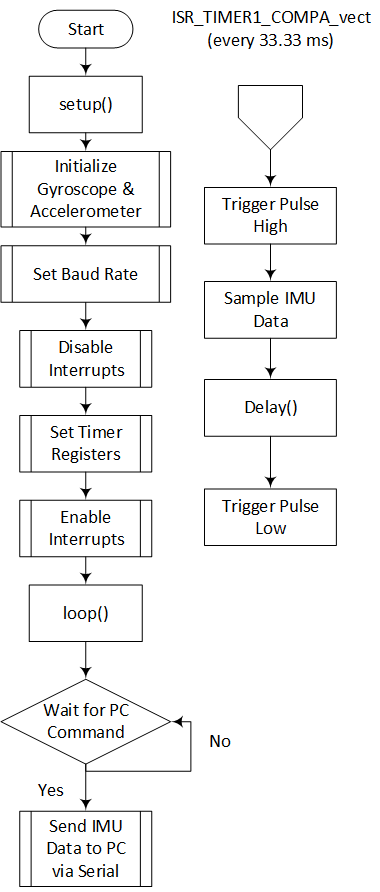
\includegraphics[width=\linewidth, height=15cm]{Figures/loop.png}
%\caption{The micro-controller program required to synchronise the sampling of the IMU and camera measurements}
%\label{fig:ISR}
%\end{wrapfigure}
This project requires a micro-controller for the following two reasons: 
\begin{itemize}
\item Digital interface with the IMU.
\item Synchronisation between the IMU and camera measurements. 
\end{itemize}

The requirements state that only a small micro-controller is required. In order to realise these requirements, the micro-controller only requires 1 GPIO pin that can be triggered by a timer interrupt as well as a I2C interface that can operate at the IMU's specified 100 Khz or 400 Khz. A board based micro-controller (like an Arduino) shouldn't only be considered, micro controllers seated in dual in-line packages (DIP) are considerably cheaper and will also be considered.  

Three micro-controllers are considered in project. These include the board based Arduino Uno SMD Rev3 and PIC32-Pinguino and the DIP  MSP430 Launchpad. Table~\ref{tab:micro} provides a general overview of some important aspects regarding theses micro-controllers.
\begin{table}[H]
\caption{General overview of the considered micro-controllers}
%\centering
\begin{tabular}{|c|c|c|c|c|}
\hline
Characteristic & Arduino Uno & Pinguino & MSP430 Launchpad & Required\\
\hline
\hline
Clock Frequency & 16 MHz & 80 MHz & 32 KHz & 400 kHz\\
\hline
%\hline
%Adapters & USB & USB & USB & USB \\
I2C (400 kHz) & yes & yes & yes & yes\\ 
\hline
IDE & yes & yes & yes & no \\
\hline
Interruptible GPIO & yes & yes & yes & 1 pin \\
\hline
Deliver Community & Large & Moderate & Small & No\\
\hline \hline
Price & R 267 & R 210 & R 120 & $\leq$ R350 \\
\hline
\end{tabular}
\label{tab:micro}
\end{table}%

Although very cheap, the MSP430 Launchpad provides the necessary specifications (one interruptible GPIO pin, I2C and minimum clock frequency) for this project, the developer community is very small, with limited the support compared to the Arduino and the Pinguino. 

The Pinguino also provides the necessary specifications but with a much larger developer community than the Launchpad. The powerful MIPS processor however will not influence this project as the micro-controller is only used for data communication. 

Although more expensive than the alternatives, the Arduino UNO SMD Rev3 depicted in Figure~\ref{fig:arduno} micro-controller still provide a suitable, low cost solution and it the controller chosen to be implemented in this project. The Arduino Uno provides the functionality necessary for this project. The user friendly integrated development environment, very helpful developer community along with source code for existing IMU implementations all contributed to the decision. 

\begin{figure}[H]
\centering
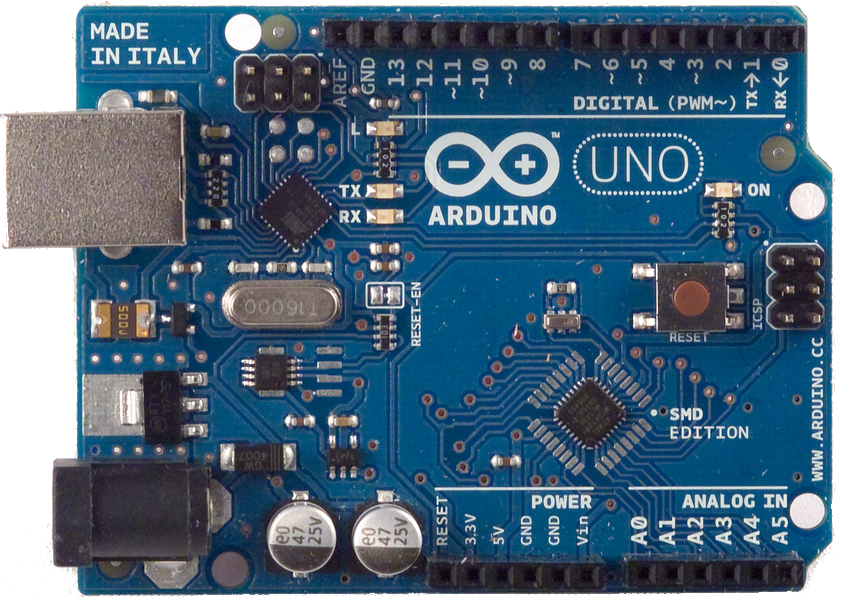
\includegraphics[width=0.42\textwidth, height=0.24\textwidth]{Figures/arduino.jpg}
\caption{Arduino UNO SMD by Arduino. Adapted from~\cite{create}.}
\label{fig:arduno}
\end{figure}
%%%%%%%%%%%%%%%%%%%%%%%%%%%%%%%%%%%%%%%%%%%%%%%%%%%%%%%%%%%%%%%%%%%%%%%%%%%
%%%%%%%%%%%%%%%%%%%%%%%%%%%%%%%%%%%%%%%%%%%%%%%%%%%%%%%%%%%%%%%%%%%%%%%%%%%
%%%%%%%%%%%%%%%%%%%%%%%%%%%%%%%%%%%%%%%%%%%%%%%%%%%%%%%%%%%%%%%%%%%%%%%%%%%

%%%%%%%%%%%%%%%%%%%%%%%%%%%%%%%%%%%%%%%%%%%%%%%%%%%%%%%%%%%%%%%%%%%%%%%%%%
%
%
%The trigger pulse is set by the micro-controller, this will be discussed next.
%%%%%%%%%%%%%%%%%%%%%%%%%%%%%%%%%%%%%%%%%%%%%%%%%%%%%%%%%%%%%%%%%%%%%%%%%%%
\newpage
\subsection{Hardware Configuration}
This Chapter seeks to discuss the necessary practical procedures undertaken to realise the system requirements defined in Chapter~\ref{sec:specs}. The system configuration as well as the data communication is done by the Arduino. The necessary code is uploaded onto the Arduino micro-controller over a USB port using the Arduino IDE. All of the code on the Arduino is written using C$++$ and compiled using g$++$.

The hardware components need to be designed in order to meet the following specifications:
\begin{itemize}
\item 30 Hz data rate.
\item Camera and IMU synchronisation.
\item Reliable data transfer from hardware to PC.
\end{itemize}

\subsubsection{Inertial Measurement Unit}\label{sec:IMUconfig}
Before any IMU measurements can be obtained, the IMU needs to be correctly configured. Communication between the micro-controller and the IMU is occurs via the I2C interface. The appropriate registers of the accelerometer and the gyroscope need to be set to resemble the configuration shown in Table~\ref{tab:imuset}.

\begin{table}[H]
\caption{Accelerometer and gyroscope register values}
\centering
%\begin{center}
\begin{tabular}{|c|c|c|c|}
\hline
Register & Value & Name & Function \\ 
\hline\hline
\multicolumn{4}{|c|}{Accelerometer} \\
\hline
0x31 & 0x09 & DATA\textunderscore FORMAT &  \pbox{7.5cm}{Set the accelerometer to $\pm 4g$ and 10 bit resolution.}\\
\hline
0x2D & 0x08 & POWER\textunderscore CTL & \pbox{7.5cm}{Set the accelerometer to measure mode with minimum power consumption.}\\
\hline
\multicolumn{4}{|c|}{Gyroscope} \\
\hline
0x16 & 0x1B & Full Scale &  \pbox{7.5cm}{Set the gyroscope to $\pm 2000^{\circ}$, 1 kHz sample rate and 100 Hz low pass filter bandwidth.}\\
\hline
\end{tabular}
%\end{center}
\label{default}
\end{table}%

The IMU sensors can now be measured and subsequently converted from analog to digital values and transferred to the PC. Both devices (accelerometer and gyroscope) are set a 10 bit resolution. This means that the analog value will be represented as 10 bits and each measurement will be stored in two separate bytes (16 bits). There are a total of 6 IMU measurements - 3 from the gyroscope and 3 from the accelerometer. A suitable baud rate must also be determined to ensure these measurement are sent to the PC within the sample period. 

The baud rate represents the number of bits per second that are transferred on a bus. The system sample period contains $\frac{1}{30} = 0.0\overline{333}$ seconds, meaning that the data sampled from the IMU needs to be transferred over the USB in-between the instances that a trigger to sample the camera is set and that 33 ms elapses. 

The I2C burst-read protocol~\cite{gyro,acc} for reading from a slave device at 100 kHz results in a 38 bits $\times$ 6 measurements $\approx$ 228 bits. At 100 kHz this data transfer consumes only 2.28 ms, well within the system sampling period of 30 Hz. The baud rate for the data transfer between the Arduino and the PC is thus essential. This project uses a baud rate of 19200 to allow all of the data to be sent though to the PC before the following system sampling instance.   
%The I2C protocol for the IMU~\cite{gyro} suggests that 60 bits per measurement are required. 
\subsubsection{Sensor Bias and Variance}
Measurement sensors often have offsets that cause a measurement \textit{bias}. These biases can however be measured and subsequently subtracted from each measurement. If each measurement is modelled with additive Gaussian RV, the bias is the mean of this noise. The procedure for measuring such a bias is quite simple: if the gyroscope is stationary, the angular velocities are expected to be zero. The procedure for measuring the accelerometer bias is slightly more difficult, as an accelerometer measures gravitational acceleration. If the accelerometer is rotated about each axis, the accelerations of the x- and y-accelerations should resemble a sinusoid due with a peak equal to the gravitational acceleration. The offset of this sinusoid is typically the measurement bias. If the accelerometer can be placed completely level, the noise on each axis can be measured. The expected value on each axis should be zero (except the z-acceleration that expected the gravitational acceleration) but the measurements will show a varying non-zero value as depicted in Figure~\ref{fig:gyrobias}. The average of this varying value is the bias. 

\begin{table}[H]
\caption{Statistical quantities of the measurement noise.}
\centering
\begin{tabular}{|c|c|c|}
\hline
Parameter & Mean & Variance\\
\hline
Acceleration $x-$axis & 0.3405 & 6.7923e-04  \\
\hline 
Acceleration $y-$axis & 0.6026 & 7.2212e-04  \\
\hline 
Acceleration $z-$axis & 0.0671 & 8.2147e-04  \\
\hline 
Gyroscope $x-$axis & 0.3587 & 0.0283 \\
\hline
Gyroscope $y-$axis & 0.0538 & 0.0188 \\
\hline
Gyroscope $z-$axis & -0.1028 & 0.0638 \\
\hline
\end{tabular}
%\end{center}
\label{tab:statimu}
\end{table}%

\begin{figure}[H]
%\centering%\begin{center}
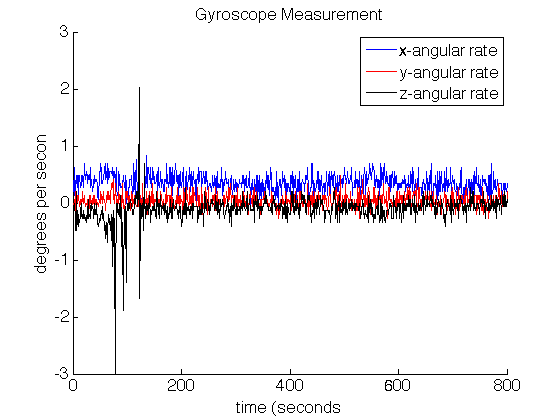
\includegraphics[width=0.49\textwidth, height=0.45\textwidth]{Figures/Gyro_bias1.png}
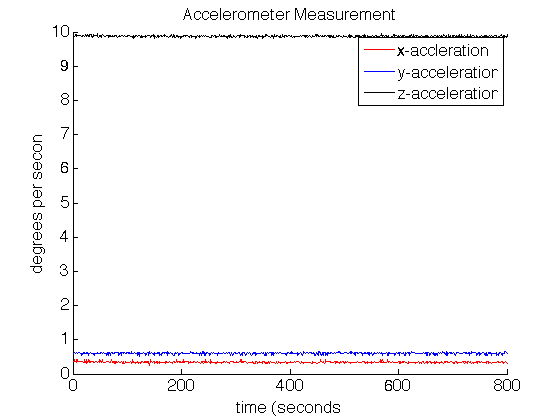
\includegraphics[width=0.49\textwidth, height=0.45\textwidth]{Figures/acc_bias_flat.png}
\caption{Left: Measurements of the stationary gyroscope. Right: Averaged measurements from the accelerometer after 3-axis individual rotations.}
\label{fig:gyrobias}
\end{figure}

%\begin{center}

The modelling of the additive noise in Chapter~\ref{sec:imu} is based statistical quantities provided in Table~\ref{tab:statimu}.
%%%%%%%%%%%%%%%%%%%%%%%%%%%%%%%%%%%%%%%%%%%%%%%%%%%%%%%%%%%%%%%%%%%%%%%%%%%
\newpage
\subsubsection{Micro-controller}\label{sec:microflow}
\begin{wrapfigure}[24]{R}{0.3\textwidth}
%\centering
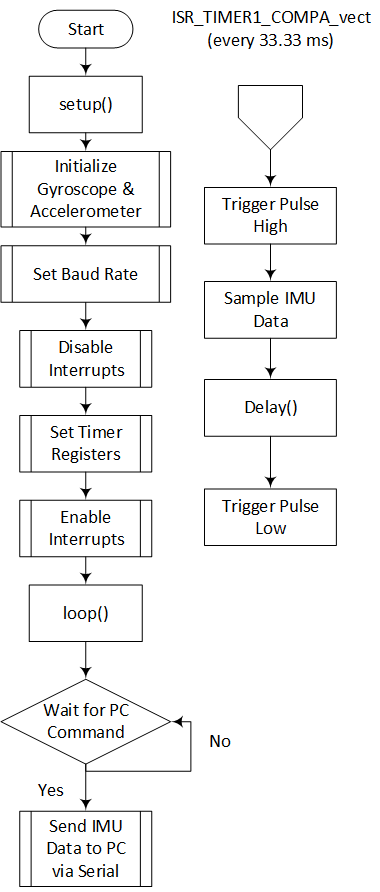
\includegraphics[width=\linewidth, height=14cm]{Figures/loop.png}
\caption{A flow diagram for the micro-controller program required to synchronise the sampling of the IMU and camera measurements.}
\label{fig:ISR}
\end{wrapfigure}
The IMU and camera measurements need to be \textit{synchronised}. A suitable method to achieve such synchronisation is to run a timer interrupt every sample period of the camera (i.e 30 Hz). The interrupt subsequently calls an interrupt service routine (ISR) that triggers a pulse to the camera to capture a frame while simultaneously sampling the IMU measurements. According to the data sheet of the camera~\cite{trigger}, a digital pulse must be set high for at least $10\mu$ seconds in order to set the moment of exposure. The exposure itself is set through external software. This procedure is shown in Figure~\ref{fig:ISR}.

The timer interrupt is required to be initiated by enabling the interrupt during the setup after the timer pre-scaler has been set to realise an interrupt ever sampling period of 33.33 ms.

Communication between the IMU and the Arduino is done via I2C. The accelerometer and the gyroscope are slave devices on the bus while the Arduino is the master. The IMU is configured according to the configuration explained in Chapter~\ref{sec:IMUconfig} in the once-off setup function before entering the infinite loop() function that waits for a command from the PC in order to send the IMU data.  
\clearpage

\newpage
\subsection{System Configuration}
\subsubsection{MonoSLAM}
The implementation discussed in this paper seeks to provide an improvement to the original implementation of MonoSLAM by Davison et al.~\cite{dav2007}. A determining factor in choosing the MonoSLAM implementation proposed by Davison et al. is the availability of the C++ based application called \textit{Scenelib} that is GNU Lesser General Public License (version 2). This allows the code to be used and updated provided that the updated version of the code is released under the same version. The original Scenelib implementation is adapted to incorporate the aspects proposed in this project as follows:
\begin{itemize}
\item The constant linear and angular velocity motion model is removed and replaced by the kinematic estimator.
\item The system is required to incorporate additional data from the IMU.
\end{itemize}

All processing of the data is done on a PC using Ubuntu 14.04 and C++ (cmake for compiling). MonoSLAM provides an interactive graphical use interface (GUI) that shows the image tracking as well as the constucted probabilistic map in real time.   
\begin{figure}[H]
\centering%\begin{center}
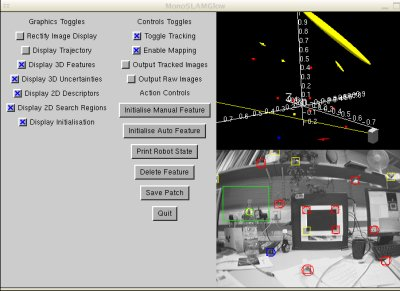
\includegraphics[width=0.8\textwidth, height=0.45\textwidth]{Figures/monoslamglow1.jpg}
\caption{The GUI of the MonoSLAM application. Adapted from~\cite{dav2007}.}
\label{fig:gyrobias}
\end{figure}
MonoSLAM requires a simple setup procedure, where a known initial pose and a known feature is required to be initialised in an initialisation file prior to system execution to provide a scale. The typical known feature is a black A5 rectangular block placed on a black background - the four corners are typically initialised as the known patch features. This image is place in a precisely known location in the environment and the location of the initialed patches are place into a initialisation file that the system reads upon execution.

In the implementation proposed in this project, the feature is placed on a (approximately) perfect vertical surface so that the IMU can be orientated with respect to the gravitational acceleration initially (level on a surface) - allowing a known initial pose.   
%%%%%%%%%%%%%%%%%%%%%%%%%%%%%%%%%%%%%%%%%%%%%%%%%%%%%%%%%%%%%%%%%%%%%%%%%%
\newpage
\section{Analysis: Testing \& Results}
\subsection{Introduction}
Due to the time constraints imposed on this project, a detailed testing analysis of the entire system is not possible. Instead, tests that seek to validate the functionality of each subsystem were implemented accordingly. The validity of the raw gyroscope and accelerometer measurements are initially inspected. Thereafter, the system sampling period as well as the data rate transfer are inspected. Additionally the validity of the kinematic state estimator is tested by providing it with simulated measurements. Finally, the issues regarding the implementation of the adapted MonoSLAM system are discussed.  

\begin{figure}[h]
\centering%\begin{center}
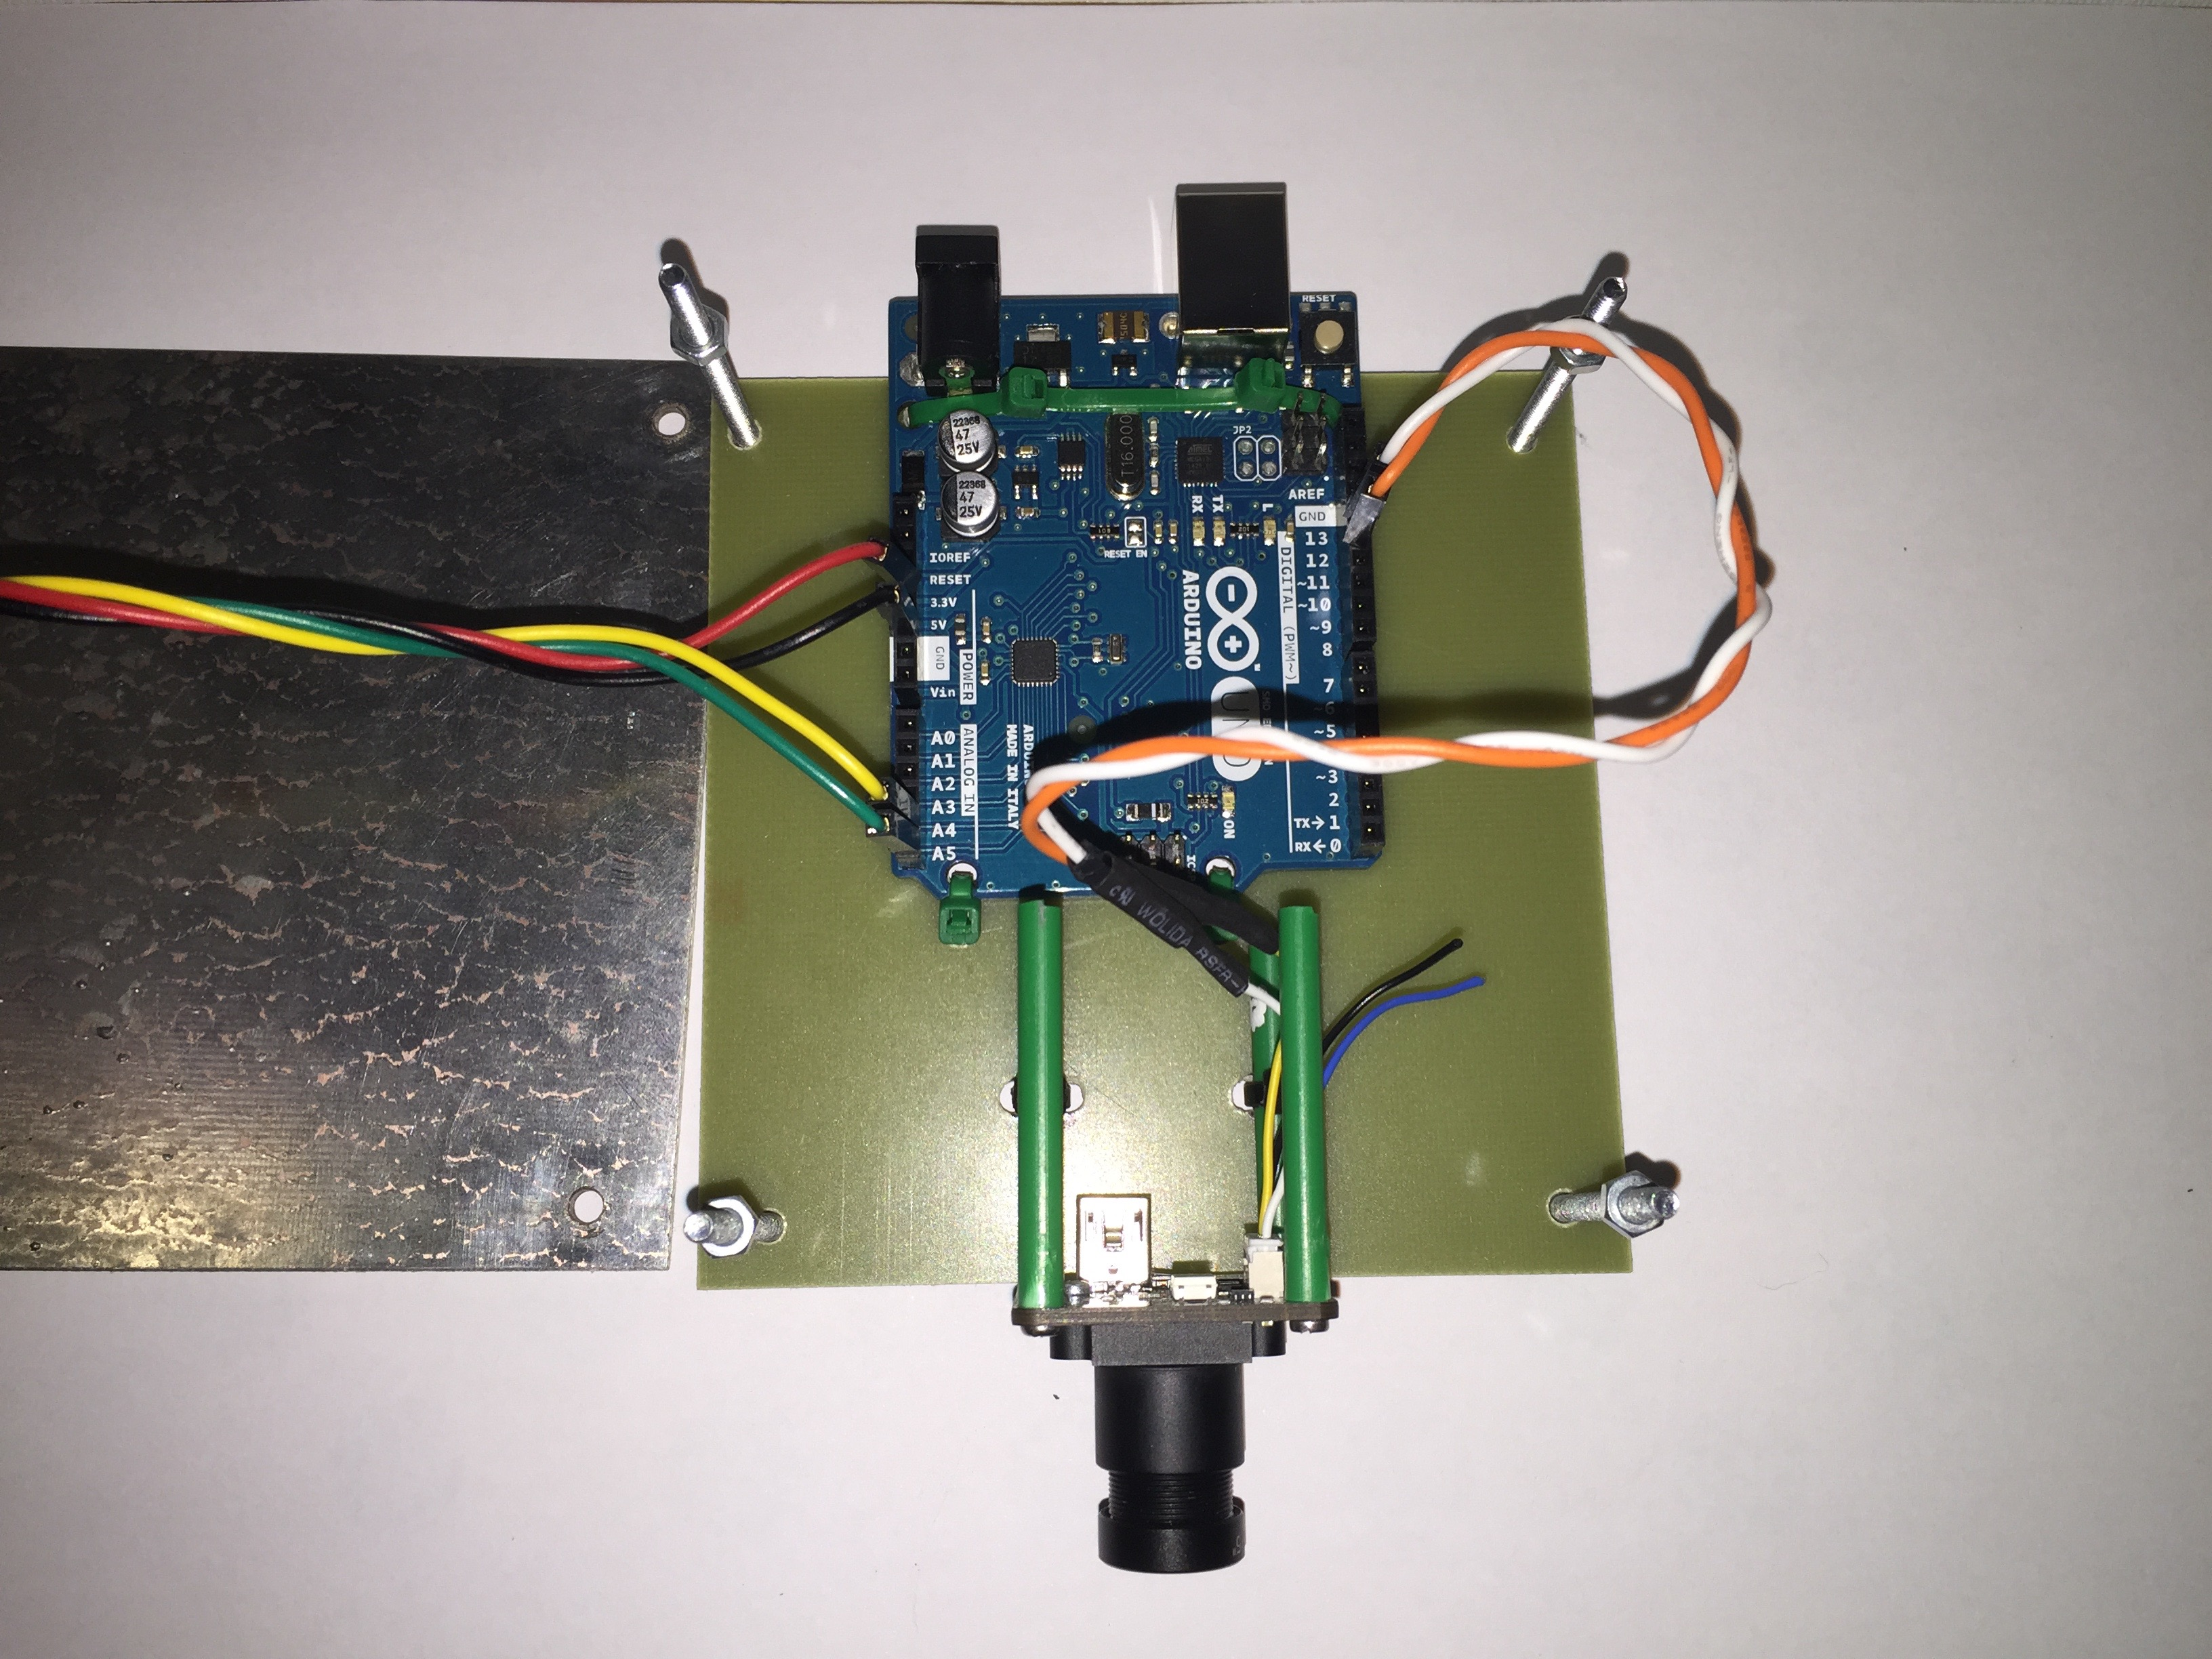
\includegraphics[width=0.49\textwidth, height=0.45\textwidth]{Figures/IMG1.jpg}
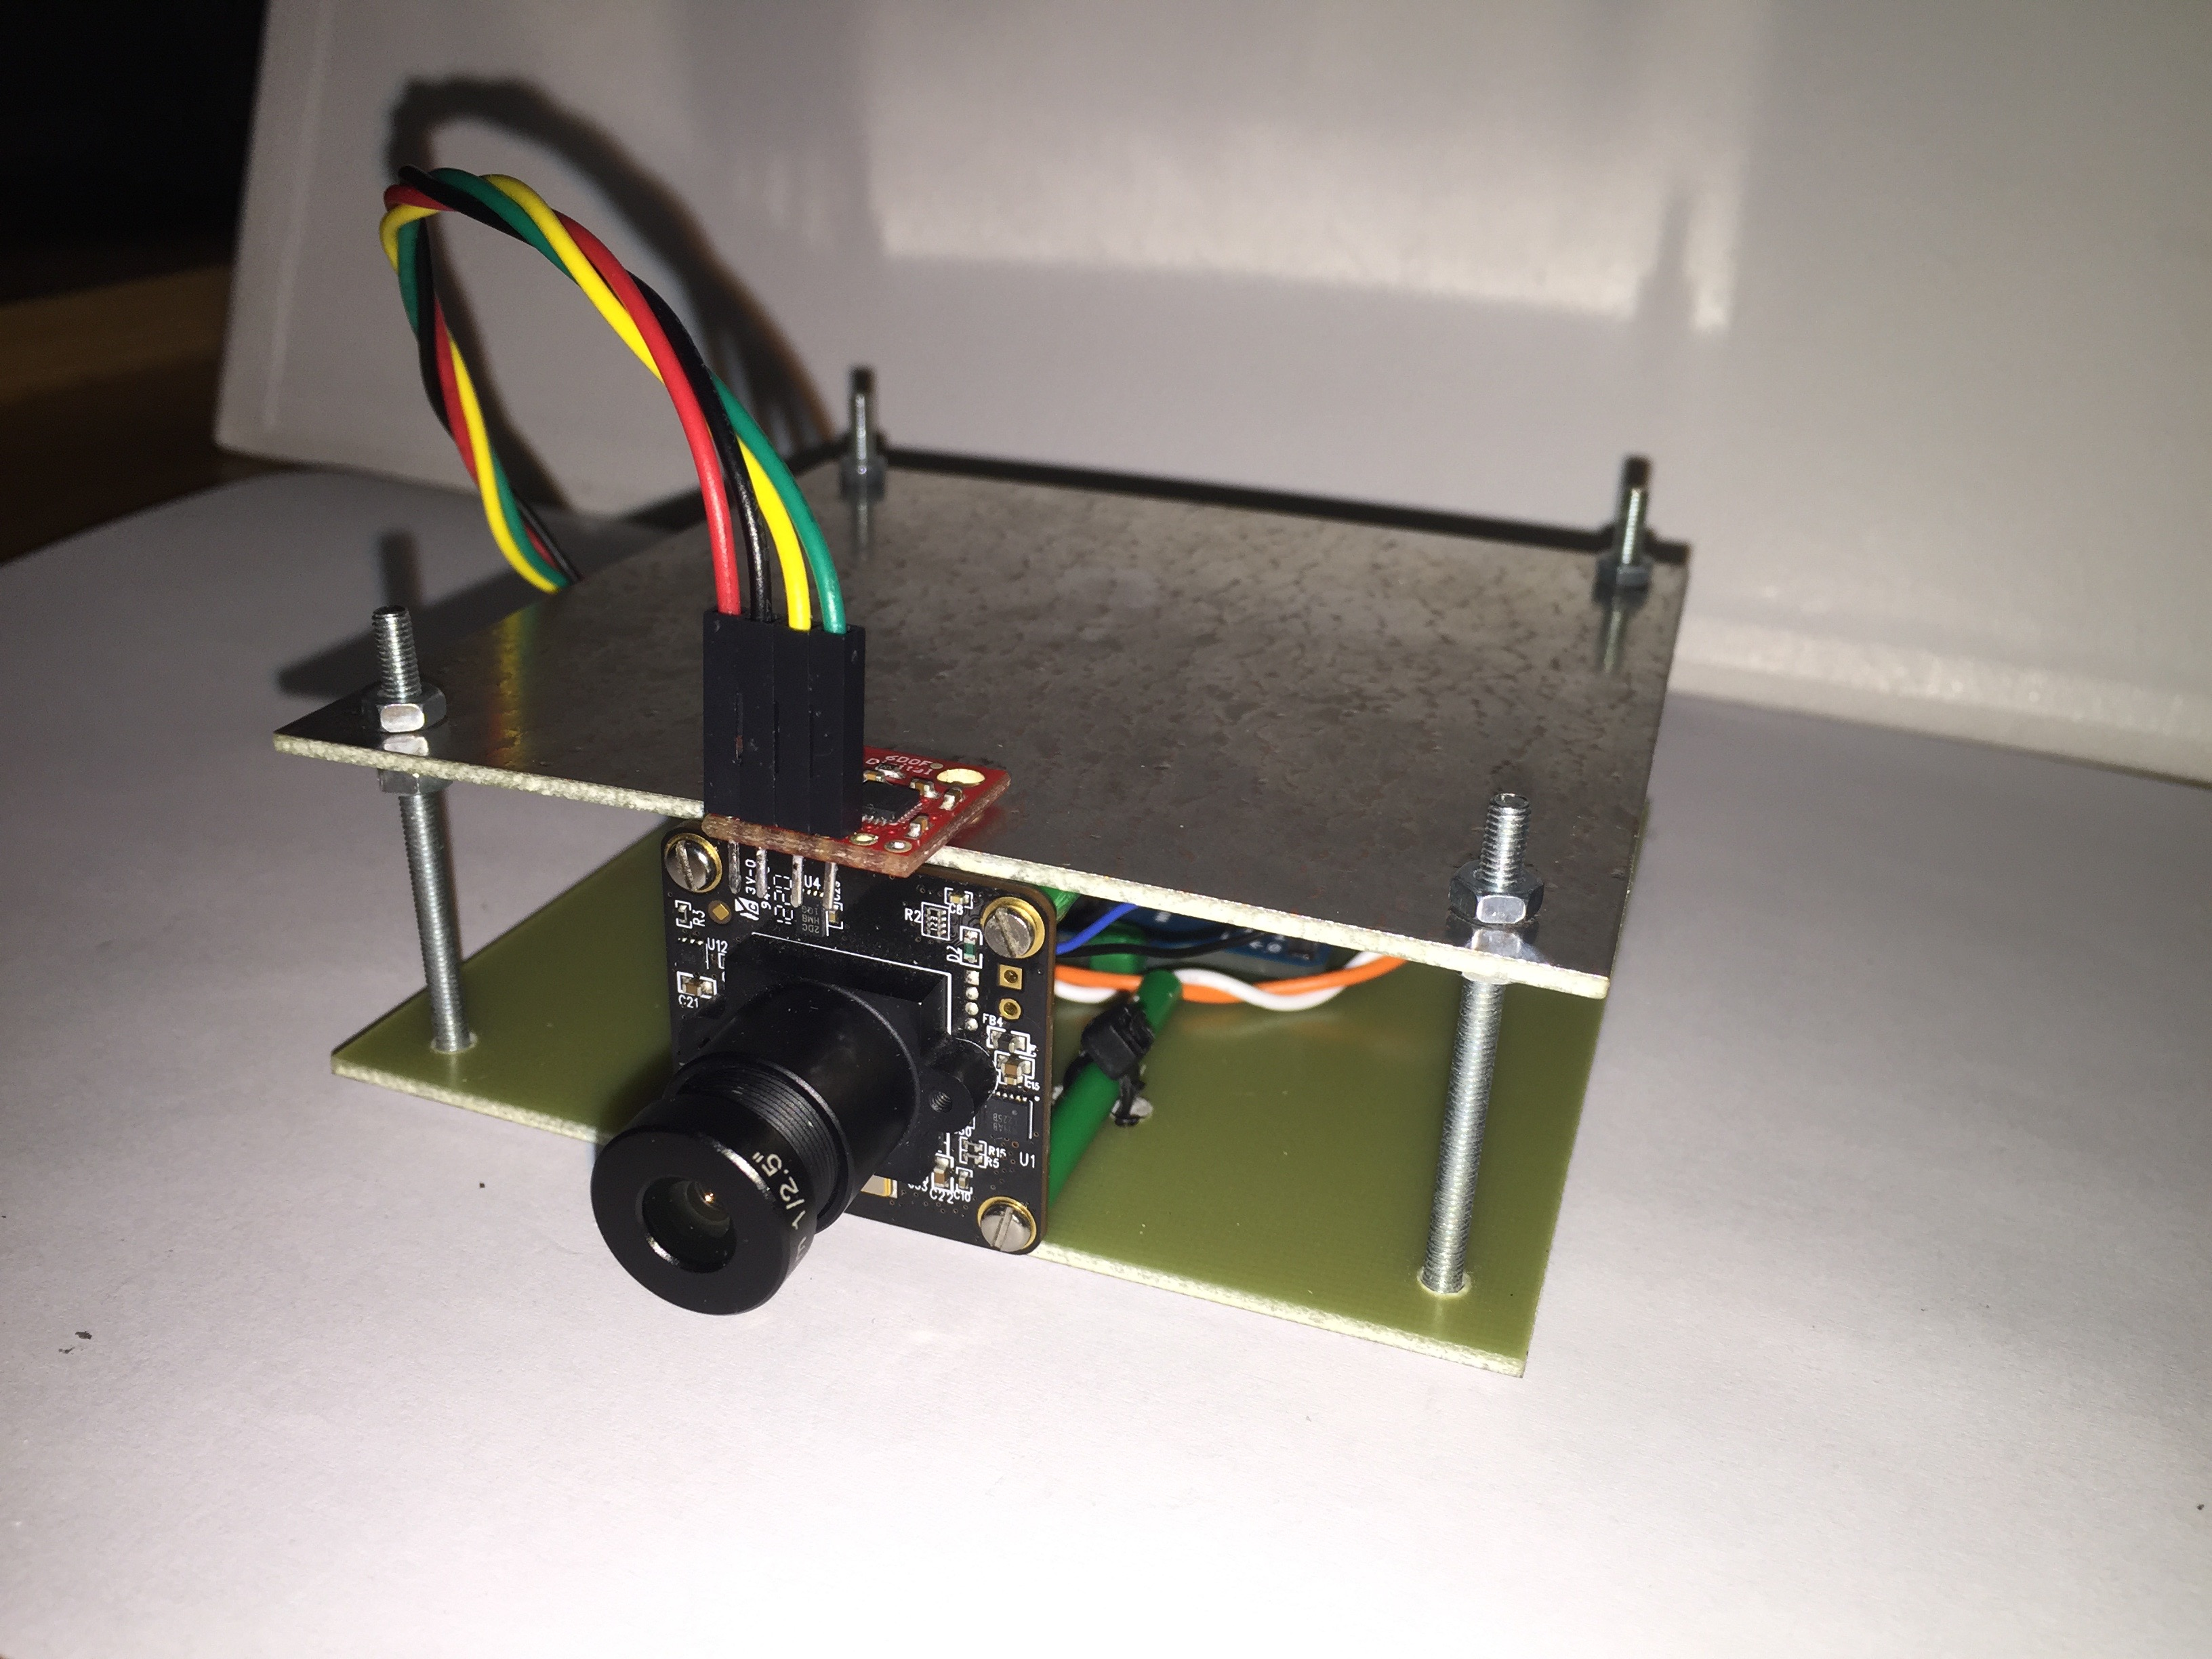
\includegraphics[width=0.49\textwidth, height=0.45\textwidth]{Figures/IMG2.jpg}
\caption{Left: Top view of the hardware components of the system system. Right: Fully constructed platform to house the hardware components of the system.}
\label{fig:gyrobias}
\end{figure}

\subsection{Subsystem testing}
The performance of the hardware components of this project requires analysis through physical measurements and simulation before being integrated into the final system. In order to successfully implement a project of this magnitude that incorporates several subsystems, it is essential that the design as well as analysis thereof is accurate. The hardware components are initially designed to meet the relevant specifications and functionality stated in Chapter~\ref{sec:impl} and Chapter~\ref{sec:system}. Thereafter, simulation and measurement equipment can be used to verify that the subsystems do indeed behave as defined in Chapter~\ref{sec:system}. This process will greatly simplify the final integration process. 

The validity of the accelerometer and gyroscope measurements are initially tested. Thereafter, the function of the micro-controller that generates a pulse and samples an IMU measurement within a system sample period is tested. Finally, the kinematic estimator is evaluated as a state estimator using simulated accelerometer and gyroscope measurements to reconstruct a trajectory.  

\subsubsection{Accuracy of Gyroscope Raw Measurements}
In order to verify the functionality of the gyroscope, the physical measurements need to be measured and analysed. It is very difficult to intuitively analyse an angular velocity. The angular displacement however, is a much better test case upon verifying that the gyroscope measurements are correct. The gyroscope can be approximately rotated at known angles and the resulting angular velocities can be numerically integrated to obtain the angular displacement. This is a suitable method of analysing whether the information obtained form the gyroscope measurements resemble the actual movements .

The following set of test conditions will utilise actual gyroscope measurements. An approximately known angular displacements will be exerted upon the IMU e.g. rotate $90^{\circ}$ about the positive x-axis. The resulting gyroscope measurements will be plotted and analysed to verify its functionality.
%The set of test conditions as are listed below (the measurements are sampled at 30 Hz): 
%\begin{enumerate}
%\item \textbf{Positive $180^{\circ}$ rotation about the x-axis:}\\
%\item \textbf{Positive $90^{\circ}$ rotation about the y-axis:}\\
%\item \textbf{Positive $90^{\circ}$ followed by a negative $90^{\circ}$ rotation about the y-axis:}\\
%\item \textbf{Positive $360^{\circ}$ rotation about the z-axis:}\\
%\end{enumerate}

Considering that the sample period is relatively small, the angular displacement $\Theta_t$ can be approximated in terms of the measured angular velocities $\psi_t$ as follows:
\begin{equation}
\begin{split}
\psi_t &= \cfrac{d\Theta_t}{dt}\\
\Theta_t &= \Delta T \psi_t
\end{split}
\end{equation}
It can also be assumed that given the small sample period, the relationship between the angular displacement and the angular velocity (velocity) can be approximated as linear.

\begin{enumerate}
\item \textbf{Positive $180^{\circ}$ rotation about the x-axis:}\\
The measurements depicted in Figure~\ref{fig:gx} show an angular position x that begins at zero and ends at approximately $180^{\circ}$ due to the rotation described by the test case.
\item \textbf{Positive $90^{\circ}$ rotation about the y-axis:}\\
The measurements depicted in Figure~\ref{fig:gy} show an angular position y that begins at zero and ends at approximately $90^{\circ}$ due to the rotation described by the test case.
\item \textbf{Positive $90^{\circ}$ followed by a negative $90^{\circ}$ rotation about the y-axis:}\\
The measurements depicted in Figure~\ref{fig:gyy} show an angular position y that begins at zero and goes to approximately $90^{\circ}$ before falling back to approximately zero due to the rotation described by the test case..
\item \textbf{Positive $360^{\circ}$ rotation about the z-axis:}\\
The measurements depicted in Figure~\ref{fig:gz} show an angular position z that begins at zero and ends at approximately $360^{\circ}$ due to the rotation described by the test case.
\end{enumerate}

Additionally, it can be observed in Figure~\ref{fig:gy1} that the rate at which the angular displacement is changing is approximately linear in all the cases. The gyroscope measurements are thus validated given that the mathematics and measurement simulation are in agreement.

\begin{figure}[H]
\centering
\begin{subfigure}[H]{0.49\textwidth}
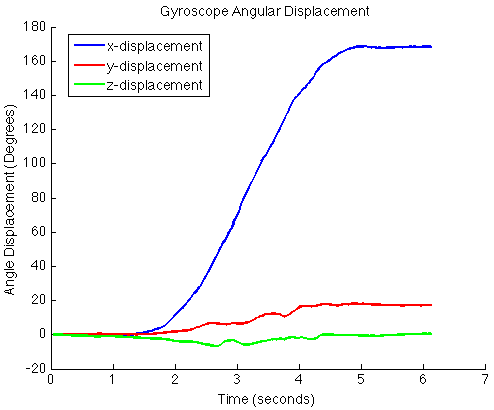
\includegraphics[width=\textwidth, height=5.5cm]{Figures/gyrox180.png} 
\caption{Angular displacement after positive $180^{\circ}$ rotation about the x-axis.}
\label{fig:gx}
\end{subfigure}
\begin{subfigure}[H]{0.49\textwidth}
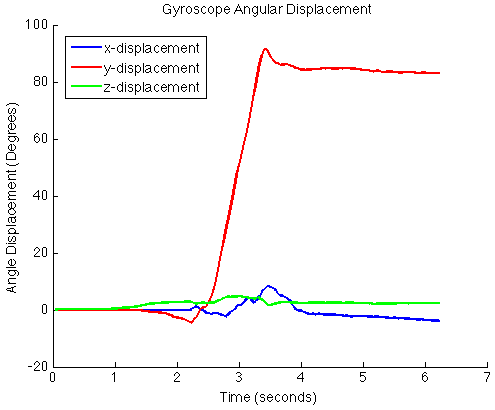
\includegraphics[width=\textwidth, height=5.5cm]{Figures/gyroy90.png}
\caption{Angular displacement after positive $90^{\circ}$ rotation about the y-axis.}
\label{fig:gy}
\end{subfigure}
\begin{subfigure}[H]{0.49\textwidth}
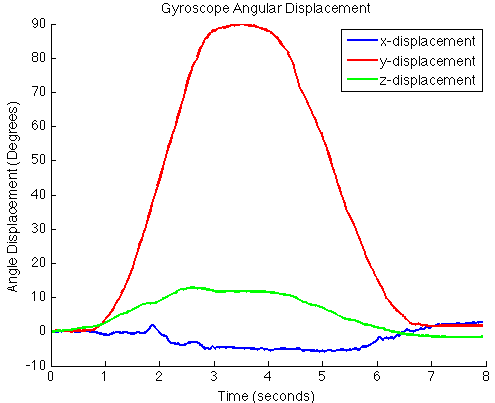
\includegraphics[width=\textwidth, height=5.5cm]{Figures/gyroy2.png}
\caption{Angular displacement after positive $90^{\circ}$ negative then $90^{\circ}$ rotation about the y-axis.}
\label{fig:gyy}
\end{subfigure} 
\begin{subfigure}[H]{0.49\textwidth}
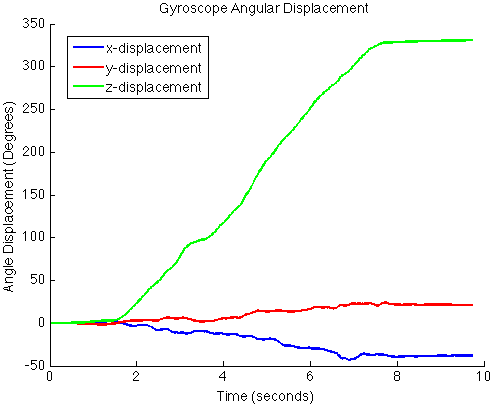
\includegraphics[width=\textwidth, height=5.5cm]{Figures/gyrox360.png}
\caption{Angular displacement after positive $360^{\circ}$ rotation about the z-axis.}
\label{fig:gz}
\end{subfigure} 
\caption{Results of the test conditions 1 depicting angular displacements from gyroscope measurements.}
\label{fig:gy1}
\end{figure}

It should be noted that the gyroscope gradually drifts over time. It is a known that the gyroscope produces a constant error that is subsequently integrated over time (upon seeking to obtain an angular position) producing a linear angular drift. It is expected though that the measurement update in the SLAM filter will account for these errors.
%%%%%%%%%%%%%%%%%%%%%%%%%%%%%%%%%%%%%%%%%%%%%%%%%%%%%%%%%%%%%%%%%%%%%%%%%%%
\subsubsection{Accelerometer Raw Measurements}
In order to verify the validity of the accelerometer, the physical measurements need to be measured and analysed. Although is is a lot easier to intuitively analyse an acceleration than an angular rate, the process of obtaining the linear acceleration is very complex. 

The accelerometer measurements may not drift over time as in the case of the gyroscope, but all accelerometer measurements incorporate gravitational acceleration. Additionally, an accelerometer cannot itself distinguish between the gravitational and linear accelerations that it measures. This typically results in the components of the gravity vector being assumed upon other axes of the accelerometer resulting in incorrect measurements. An additional sensor is typically required - in this instance the gyroscope. The idea is to measure the degree by which the orientation changes (using the gyroscope measurements), and at each instance subtract the gravity vector. 

As previously mentioned however, the gyroscope drifts over time. The orientation at each time instance needs to be precisely known in order to successfully subtract the gravitational acceleration. The error in orientation then, causes linear acceleration measurements that cannot accurately reconstruct the position of a robot. 

This issue was realised late in this project and couldn't be rectified due to the hard deadline of the project. An alternative suggestion was to account for this problem in the context of this project, by substantially increasing the variance of the accelerometer noise. This procedure tells the EKF that you are very uncertain regarding this measurement and the EKF will take this into consideration upon obtaining the optimal weighting of the state estimate.

\subsubsection{System Sampling Period}
In order to verify that the system sampling period is according to the desired requirements (30 Hz), a set of measurements need to be obtained measuring the timer-interrupt realised by the micro-controller in Chapter~\ref{sec:microflow}. An oscilloscope can be used to measure the port that triggers the camera's GPIO pin. This pin expects a pulse with a width of at least $10\mu$s repeated at least every 30 Hz.
\begin{figure}[h]
\centering%\begin{center}
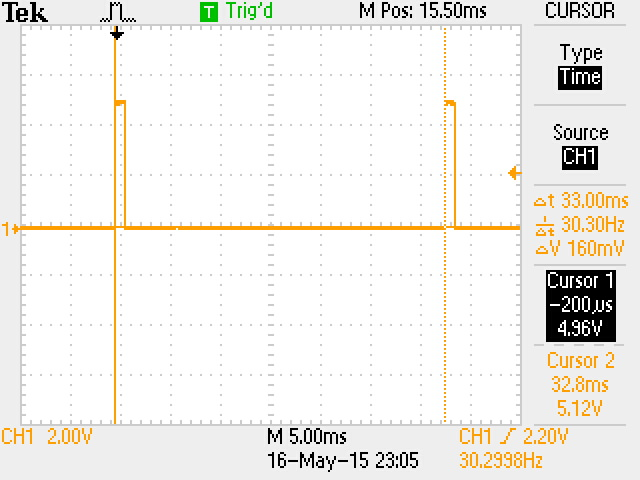
\includegraphics[width=0.49\textwidth, height=0.33\textwidth]{Figures/TEK2.jpg}
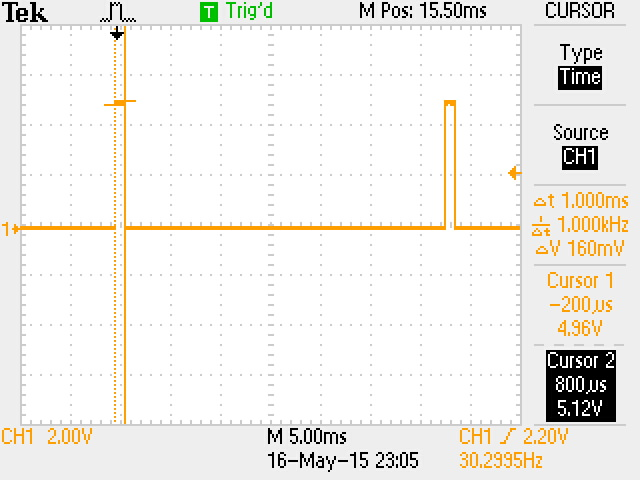
\includegraphics[width=0.49\textwidth, height=0.33\textwidth]{Figures/TEK3.jpg}
\caption{Left: Measurement depicting the frequency between the pulses - 30.3 Hz Right: Measurement depicting the width of the pulses - $10\mu$s.}
\label{fig:pinmeas}
\end{figure}
\subsubsection{Sufficient Data Transfer Speed}
In order to verify that the data transfer of the IMU measurements onto the PC system are within sampling period, a set of measurements need to be obtained measuring the data transfer by the micro-controller in Chapter~\ref{sec:microflow}. An oscilloscope can be used to measure the transmit port of the UART. A full set of IMU measurements (3 gyroscope and 3 accelerometer) are sampled and subsequently transmitted on this pin. The data should be transferred to the PC within the system sampling period.

\begin{figure}[H]
\centering%\begin{center}
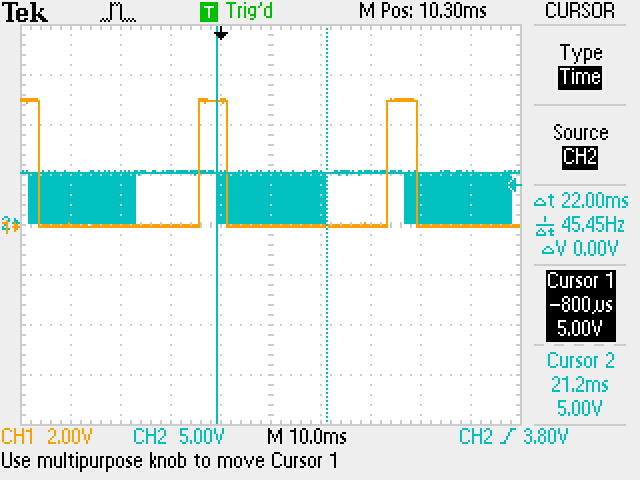
\includegraphics[width=0.49\textwidth, height=0.33\textwidth]{Figures/TEK5.jpg}
\caption{Measurement depicting the time taken for a single, full IMU data measurement to be sampled and sent to the PC.}
\label{fig:samp}
\end{figure}

Figure~\ref{fig:samp} shows that the full data transfer is well within the system sampling period and the speed of transmission is thus sufficient.
%%%%%%%%%%%%%%%%%%%%%%%%%%%%%%%%%%%%%%%%%%%%%%%%%%%%%%%%%%%%%%%%%%%%%%%%%%
%\newpage
%\subsubsection{Serial Communication}
%Each of the hardware subsystems use serial communication to transfer of data. All relevant data from the subsystems is required to be transferred to the PC, where the SLAM algorithm is being run. The project description requires operation at 30 Hz. The individual subsystems are required to be configured so that it transfers all its relevant data to PC before the sample period expires. It is essential however, that the data from each subsystem remains in sync.
%
%Table~\ref{tab:serialcom} shows each hardware subsystem, the method of serial architecture used and the amount of data required to be transferred every sampling instance $f = 30$Hz:   
%\begin{table}[H]
%\caption{Serial Communication Architectures per device}
%\begin{center}
%\begin{tabular}{|c|c|c|}
%\hline
%Subsystem & Serial Architecture & Data (Bytes) \\
%\hline \hline
%Micro-controller & USB & \\
%\hline 
%CMOS camera & USB & \\
%\hline
%IMU & I2C & \\ 
%\hline
%\end{tabular}
%\end{center}
%\label{tab:serialcom}
%\end{table}%

%\begin{table}[H]
%\caption{Single-Byte I2C Write Cycle}
%\begin{center}
%\begin{tabular}{|c|c|c|c|c|c|c|c|c|}
%\hline
%master & start & device adr + write & & register adr & & data & & stop \\ 
%\hline
%slave & & & ack & & ack & & ack &  \\
%\hline
%\end{tabular}
%\end{center}
%\label{tab:read}
%\end{table}
%\begin{table}[H]
%\caption{Single-Byte I2C Read Cycle}
%\begin{center}
%\begin{tabular}{|c|c|c|c|c|c|c|c|c|c|c|c|}
%\hline
%master & start & device add & & register adr & & start & register adr & & & $\overline{\text{ack}}$ & stop \\ 
%\hline
%slave& & & ack & & ack & & & ack & data &  &\\
%\hline
%\end{tabular}
%\end{center}
%\label{tab:write}
%\end{table}
%%%%%%%%%%%%%%%%%%%%%%%%%%%%%%%%%%%%%%%%%%%%%%%%%%%%%%%%%%%%%%%%%%%%%%%%%%
\newpage
\subsection{Simulation}
This study seeks to investigate the performance of the kinematic estimator as a state transition model. An EKF-based kinematic estimator \textit{simulation} is designed to meet the following specifications:
\begin{itemize}
\item Simulated measurements are calculated by adding noise to the states. 
\item The kinematic estimator should precisely track a trajectory of a robot from simulated IMU measurements, given that there is no uncertainty regarding the system. 
\end{itemize}

In order to effectively analyse its performance, a simulation of an EKF that uses a kinematic estimator as the state transition model is run under a set of test conditions. These conditions will accurately analyse the performance of the kinematic estimator with regard to the aforementioned design specifications. A functional diagram of the EKF-based kinematic estimator (based on Equation~\ref{eq:trmod}) is shown in Figure~\ref{fig:kindiag}. The kinematic estimator is incorporated within the control update of the EKF. %A set of \textit{simulated} inertial measurements will initially be inserted into the kinematic estimator simulation and the resulting trajectory will be plotted to provide better insight. Thereafter a set of random measurements will be inserted into the kinematic estimator with  
\begin{figure}[htbp]
\begin{center}
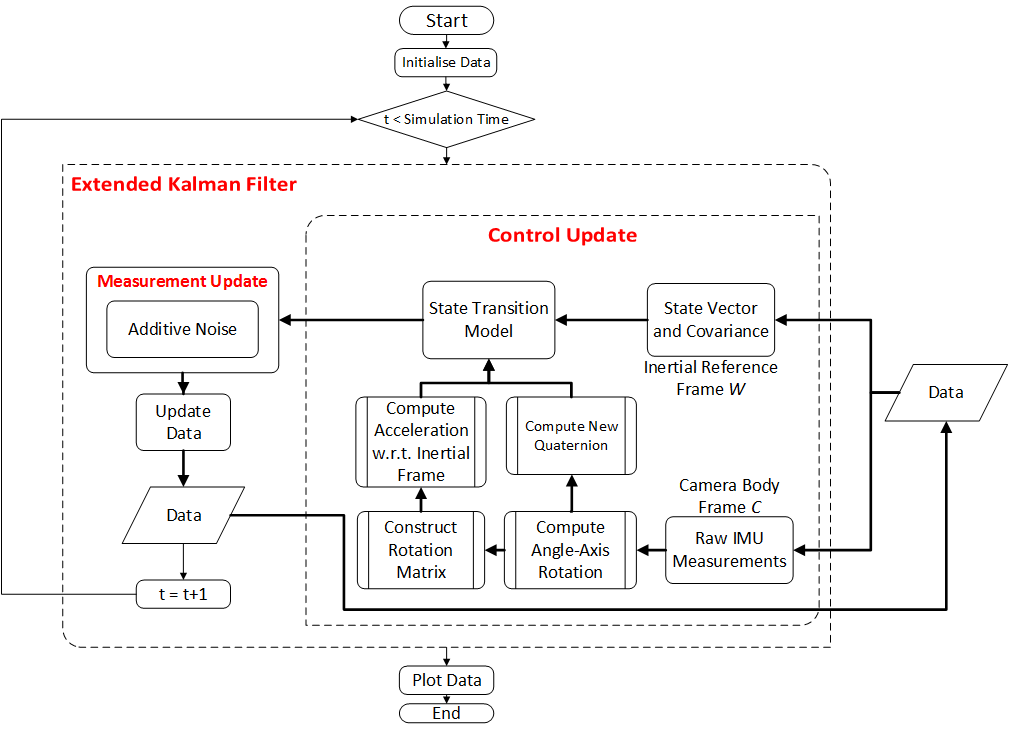
\includegraphics[width=\textwidth, height=0.8\textwidth]{Figures/Drawing3.png}
\caption{EKF using a kinematic estimator to provide the control update.}
\label{fig:kindiag}
\end{center}
\end{figure}

\newpage
\subsubsection{Recovering a Trajectory from Simulated IMU Measurements}
 will provide simulated gyroscope and accelerometer measurements in a noiseless environment. The EKF simulation measurement model is defined as a mapping of the state vector with additive noise. With no uncertainty regarding the measurement or process noise then, the simulated state estimates should exactly resemble the actual state vector. 

The expected outcome then, is that the kinematic estimator will precisely track a given robot trajectory. This trajectory will be simply defined so that the results can be accurately analysed. 
\\\\
The length of a simulation is 10 seconds at 30 Hz or 300 samples. The initial position is always $\textbf{r}^W$ = \{0 0 0\} with an orientation quaternion of $\textbf{q}^{WC} =$ \{1 0 0 0\}): %The trajectory of the can thus qualitatively analysed to predict the performance of the kinematic estimato.

%begin{enumerate}
%\item \textbf{1 metre per second squared x-acceleration:}\\
%The trajectory is expected to only move along the positive x-axis. Newtons equations of motions suggest that the displacement of the robot due to a constant acceleration is:
%\begin{equation}
%x = x_0 + \cfrac{t^2}{2} = 0 + \cfrac{10^2}{2} = 50 \text{m}
%\end{equation}
%\item \textbf{1 metre per second squared x-acceleration with sudden positive 90 degree rotation about the y-axis:}\\
%The trajectory is expected to initially move along the positive x-axis after which the positive 90 degree rotation about the y-axis will rotate the robot frame so that the trajectory only moves along the negative z-axis. 
%\item \textbf{1 metre per second squared x-acceleration with three consecutive 90$^{\circ}$ rotations about the z-axis:}\\
%The trajectory is expected to initially move along the positive x-axis until the first positive 90$^{\circ}$ degree rotation about the z-axis rotates the robot frame so that the trajectory only moves along the positive y-axis. A second positive 90$^{\circ}$ rotation about the z-axis rotates the robot frame so that the trajectory then moves along the negative x-axis. The final positive 90 degree rotation about the z-axis rotates the robot frame so that the trajectory only moves along the negative y-axis. If the time steps between the rotations are equal, a block figure trajectory is expected in the plane of rotation.    
%\end{enumerate}
%\newpage
%\subsubsection{Test 1: Results and Analysis}
\begin{enumerate}
%\item \textbf{1 metre per second x-acceleration:}\\
%The simulation depicted in Figure~\ref{fig:xacc} shows a trajectory only moving along the positive x-axis. The final x-position is given to be 50 metres, exactly the predicted value. Furthermore, the estimated trajectory directly tracks the true trajectory.  
%\item  \textbf{1 metre per second x-acceleration with sudden 90 degree rotation about the y-axis:}\\
%The simulation depicted in Figure~\ref{fig:yrot} shows a trajectory that initially moves along the positive x-axis before proceeding to move along the negative z-axis. Again, the estimated trajectory directly tracks the true trajectory.
\item  \textbf{1 metre per second squared x-acceleration with three consecutive 90$^{\circ}$ rotations about the z-axis:}\\   
The simulation depicted in Figure~\ref{fig:zplane} shows a square in the z-plane. This suggests that the trajectory incorporates three 90$^{\circ}$ rotations about the z-axis as the robot is moving at a constant acceleration with respect to its own reference frame. The simulation depicted in Figure~\ref{fig:zplanex} confirms that there is an initial acceleration in the x direction, before a change in direction. The estimated trajectory directly tracks the true trajectory.
\end{enumerate}
\begin{figure}[H]
%\centering
%\begin{subfigure}[H]{0.49\textwidth}
%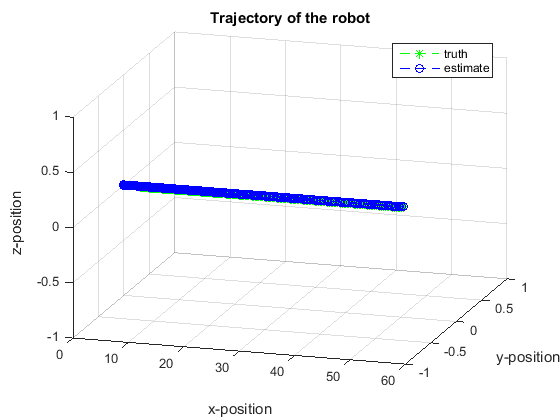
\includegraphics[width=\textwidth, height=5.8cm]{Figures/accx_1_traj.png} 
%\caption{Trajectory: 1 $\text{m/s}^2$ x-acceleration.}
%\label{fig:xacc}
%\end{subfigure}
%\begin{subfigure}[H]{0.49\textwidth}
%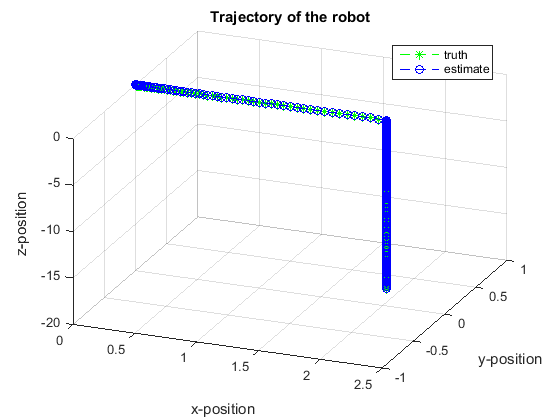
\includegraphics[width=\textwidth, height=5.8cm]{Figures/90rotx_traj.png}
%\caption{Trajectory: 1 $\text{m/s}^2$ x-acceleration with sudden $90^{\circ}$ rotation about the y-axis.}
%\label{fig:yrot}
%\end{subfigure}
\centering
\begin{subfigure}[H]{0.49\textwidth}
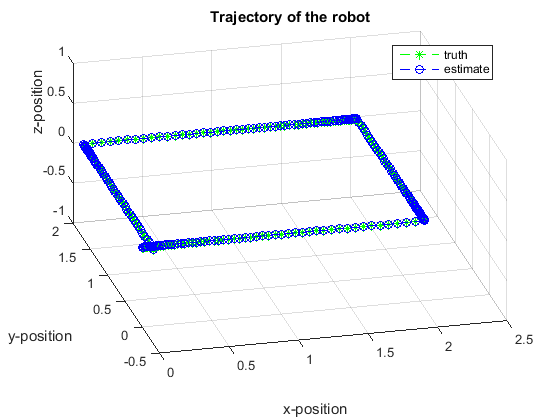
\includegraphics[width=\textwidth, height=8cm]{Figures/xy_block_traj.png}
\caption{Trajectory: 1 $\text{m/s}^2$ x-acceleration with three consecutive $90^{\circ}$ rotations about the z-axis.}
\label{fig:zplane}
\end{subfigure} 
\begin{subfigure}[H]{0.49\textwidth}
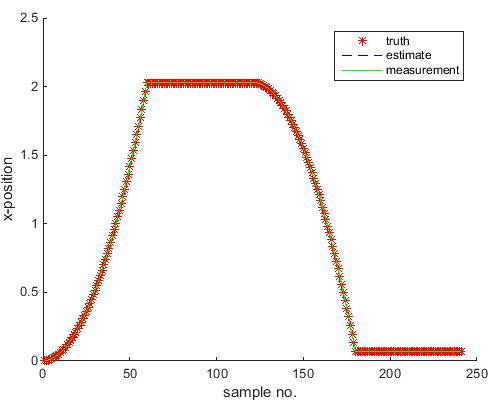
\includegraphics[width=\textwidth, height=8cm]{Figures/xy_block_x.png}
\caption{x-position: 1 $\text{m/s}^2$ x-acceleration with three consecutive $90^{\circ}$ rotations about the z-axis.}
\label{fig:zplanex}
\end{subfigure} 
\caption{Results of the test conditions 1 depicting zero-uncertainty.}
\label{fig:sim1}
\end{figure}
%%%%%%%%%%%%%%%%%%%%%%%%%%%%%%%%%%%%%%%%%%%%%%%%%%%%%%%%%%%%%%%%%%%%%%%%%%
%%%%%%%%%%%%%%%%%%%%%%%%%%%%%%%%%%%%%%%%%%%%%%%%%%%%%%%%%%%%%%%%%%%%%%%%%%
\newpage
\subsection{MonoSLAM}
This implementation of section in practice proved to be a very challenging part of this project. As a result of the time constraints imposed on this project, a functional system upon which fundamental tests could be undertaken was not possible. Initially, the system imposed a number of challenges that were not related to the theoretical concepts of this project. These challenges are listed as follows:
\begin{itemize}
\item Ubuntu 14.04 no longer supports ffmpeg as default and has replace this with libav which doesn't support the USB camera feeds used by Scenlib. A previous version of Scenelib was required to be used that only uses saved image sequences.
\item The numerical libraries that are used by Davison et al. (Oxford universities vision workshop (VW)) is outdated and has no meaningful documentation. The existing code had to be studied in order to understand the library well enough to incorporate it within the proposed alterations to the project.
\item It was initially very difficult to understand the Scenelib library due to its complexity, lack of a comprehensive documentation and my lack of experience using C++.    
\end{itemize}
 
The kinematic state estimator was however implemented successfully within the control update of Scenelib with the results from the simulation depicting the results in Scenelib given the same simulated variables. Figure~\ref{fig:davsim} depicts the simulations of the simulation in Matlab against the simulation of Davision given precisely the simulated variables:

\begin{figure}[h]
\centering%\begin{center}
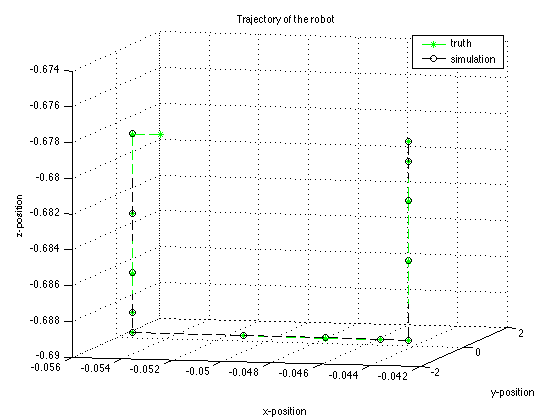
\includegraphics[width=0.49\textwidth, height=0.45\textwidth]{Figures/dav1.png}
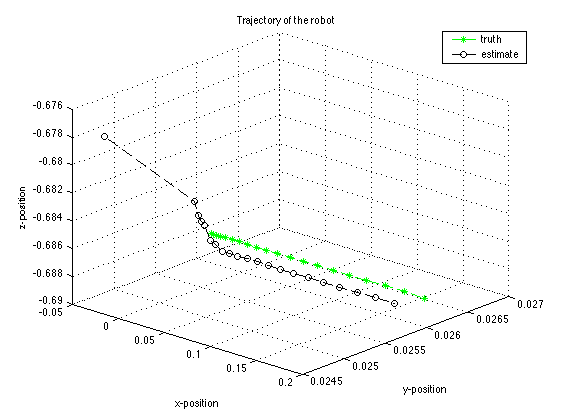
\includegraphics[width=0.49\textwidth, height=0.45\textwidth]{Figures/dav2.png}
\caption{Left: Trajectory of the simulation against the results of the Scenelib control update. Right: Trajectory of the simulation against the results of the Scenelib control update.}
\label{fig:davsim}
\end{figure}

The minor differences in the value are possibly due to rounded values. The direness are minimal though and the two simulations can be approximated as identical.

The measurement update of the MonoSLAM system in Scenelib contained errors in the re-projection of the image patches for matching. As a result, accurate matching never occurs and the system terminates. It is concluded that the distortion model approximated dorm Davision et al. in Equation~\ref{eq:raddist} incorporates too much radial distortion and as a result projection of images are incorrect. This problem was however identified too late in the project to correct given the hard deadline. 
%%%%%%%%%%%%%%%%%%%%%%%%%%%%%%%%%%%%%%%%%%%%%%%%%%%%%%%%%%%%%%%%%%%%%%%%%%
%%%%%%%%%%%%%%%%%%%%%%%%%%%%%%%%%%%%%%%%%%%%%%%%%%%%%%%%%%%%%%%%%%%%%%%%%%
%%%%%%%%%%%%%%%%%%%%%%%%%%%%%%%%%%%%%%%%%%%%%%%%%%%%%%%%%%%%%%%%%%%%%%%%%%
%%%%%%%%%%%%%%%%%%%%%%%%%%%%%%%%%%%%%%%%%%%%%%%%%%%%%%%%%%%%%%%%%%%%%%%%%%
\newpage
\section{Conclusions and Recommendations}
\subsection{Introduction}
This chapter concludes all the work conducted throughout this project and provides recommendations on further improvements to the project.

\subsection{Conclusion}
The core of the project, namely the kinematic state estimator along with the individual hardware subsystems was proven successful as far as possible. The final implementation of the MonoSLAM system however was not successful. The failure to successfully implement the proposed system is possibly be due to various individual factors, both practical, theoretical and time, as well as a combination of these factors. The discussion that follows provides the possible causes of the inability to realise a successful SLAM implementation.

The accelerometer used in this project aims to measure the linear accelerations of a body. This process proved to be a lot more difficult than expected as there is now possible way to determine the linear acceleration unless the orientation is precisely known. The method used in this project proposed to use the measurements from the gyroscope to obtain the changes in orientation. If the initial orientation is known (this is a requirement of the SLAM algorithm proposed in this project) the measurements form the gyroscope can be used to obtain the change in orientation. The gravity vector can subsequently be subtracted at each time step as its orientation with respect to the reference frame is always the negative z-direction. The gyroscope measurements however provide a constant error that is integrated with time resulting in drift and subsequently, inaccurate orientation estimates upon which the system depends in order to remove the gravity vector. This problem was initially accounted for by vastly increasing the uncertainty of the measurements but could possibly be overcome by additionally incorporating a magnetic sensor (magnetometer). A magnetometer can obtain additional information regarding the orientation of gravity by measuring the magnetic fields surrounding the earth. This process is common in inertial navigation and can be realised with an inexpensive sensor and minor additions to the equivalent control input calculations. 

Furthermore the failure of the MonoSLAM Scenelib system to conduct a thorough SLAM solution could be attributed to the fact that the radial distortion approximation assumed from Davison et al.~\cite{dav2007} causes an incorrect re-projection that is used to subsequently match the feature in the frames that follow. A distortion model suited to the specific camera used in this implementation was not researched accordingly. This problem can be corrected by obtaining a suitable distortion model to allow successful reproduction of the features for the best chance of correlation.

Finally it should be noted that even though a full implementation of the system was not achieved, the functional components of the system (besides the accelerometer) as well as the core kinematic estimator were implemented successfully as far as possible given the time constraints. These components include an IMU (besides the accelerometer) that can approximately measure an angular displacement, a Matlab simulation of the kinematic estimator that is also correctly implemented on Scenelib and the micro-controller that successfully achieves the system sampling period.

\subsection{Recommendations}
 Although the kinematic estimator MonoSLAM was not fully realised, many of the systems were successfully designed and accordingly implemented. The factors influencing the failure to fully implement the system are given as follows:
\begin{itemize}
\item Inaccurate accelerometer measurements based on gravity vector. The gyroscope error over time prevents accurate orientation estimates to correctly subtract the gravity vector.
\item The incorrectly assumed radial distortion. 
\end{itemize}
 
The successfully designed and implemented subsystems however provide a good basis for the project to be completed with additional time with possible further development. The project objectives that were achieved are as follows:
\begin{itemize}
\item \textbf{Performing an overview on the current techniques used to realise SLAM} \\
In order to understand how SLAM is implemented, an understanding of probability theory and state estimation is required. These concepts - specifically recursive state estimation and the Bayes filter - need to be researched and analysed before choosing a suitable technique to implement.
\item \textbf{Analysis of the kinematic estimator as an alternative motion model}\\
A kinematic estimator is suggested as a alternative motion model. The kinematic estimator needs to be researched, mathematically derived and simulated. The results from the simulation should correspond to the mathematical derivation. The advantages and disadvantages of the kinematic estimator also need to be investigated.
\item \textbf{Hardware Design of the System} \\
The kinematic estimator requires additional measurements obtained from an IMU. The IMU is required to interface with the PC via a micro-controller. The micro-controller allows precise synchronisation between the images sampled by the camera and the IMU measurements. A functional diagram of the system's hardware components are depicted in Figure~\ref{fig:sys}.  
\end{itemize}

       



%%%%%%%%%%%%%%%%%%%%%%%%%%%%%%%%%%%%%%%%%%%%%%%%%%%%%%%%%%%%%%%%%%%%%%%%%
%%%%%%%%%%%%%%%%%%%%%%%%%%%%%%%%%%%%%%%%%%%%%%%%%%%%%%%%%%%%%%%%%%%%%%%%%%
%%%%%%%%%%%%%%%%%%%%%%%%%%%%%%%%%%%%%%%%%%%%%%%%%%%%%%%%%%%%%%%%%%%%%%%%%%
%%%%%%%%%%%%%%%%%%%%%%%%%%%%%%%%%%%%%%%%%%%%%%%%%%%%%%%%%%%%%%%%%%%%%%%%%%
%%%%%%%%%%%%%%%%%%%%%%%%%%%%%%%%%%%%%%%%%%%%%%%%%%%%%%%%%%%%%%%%%%%%%%%%%%
%%%%%%%%%%%%%%%%%%%%%%%%%%%%%%%%%%%%%%%%%%%%%%%%%%%%%%%%%%%%%%%%%%%%%%%%%%
%%%%%%%%%%%%%%%%%%%%%%%%%%%%%%%%%%%%%%%%%%%%%%%%%%%%%%%%%%%%%%%%%%%%%%%%%%
%%%%%%%%%%%%%%%%%%%%%%%%%%%%%%%%%%%%%%%%%%%%%%%%%%%%%%%%%%%%%%%%%%%%%%%%%%
%%%%%%%%%%%%%%%%%%%%%%%%%%%%%%%%%%%%%%%%%%%%%%%%%%%%%%%%%%%%%%%%%%%%%%%%%%
%%%%%%%%%%%%%%%%%%%%%%%%%%%%%%%%%%%%%%%%%%%%%%%%%%%%%%%%%%%%%%%%%%%%%%%%%%
%%%%%%%%%%%%%%%%%%%%%%%%%%%%%%%%%%%%%%%%%%%%%%%%%%%%%%%%%%%%%%%%%%%%%%%%%%
%%%%%%%%%%%%%%%%%%%%%%%%%%%%%%%%%%%%%%%%%%%%%%%%%%%%%%%%%%%%%%%%%%%%%%%%%%
%%%%%%%%%%%%%%%%%%%%%%%%%%%%%%%%%%%%%%%%%%%%%%%%%%%%%%%%%%%%%%%%%%%%%%%%%%
%%%%%%%%%%%%%%%%%%%%%%%%%%%%%%%%%%%%%%%%%%%%%%%%%%%%%%%%%%%%%%%%%%%%%%%%%%
%%%%%%%%%%%%%%%%%%%%%%%%%%%%%%%%%%%%%%%%%%%%%%%%%%%%%%%%%%%%%%%%%%%%%%%%%%
%%%%%%%%%%%%%%%%%%%%%%%%%%%%%%%%%%%%%%%%%%%%%%%%%%%%%%%%%%%%%%%%%%%%%%%%%%
%%%%%%%%%%%%%%%%%%%%%%%%%%%%%%%%%%%%%%%%%%%%%%%%%%%%%%%%%%%%%%%%%%%%%%%%%%
%%%%%%%%%%%%%%%%%%%%%%%%%%%%%%%%%%%%%%%%%%%%%%%%%%%%%%%%%%%%%%%%%%%%%%%%%%
%%%%%%%%%%%%%%%%%%%%%%%%%%%%%%%%%%%%%%%%%%%%%%%%%%%%%%%%%%%%%%%%%%%%%%%%%%
%%%%%%%%%%%%%%%%%%%%%%%%%%%%%%%%%%%%%%%%%%%%%%%%%%%%%%%%%%%%%%%%%%%%%%%%%%
%%%%%%%%%%%%%%%%%%%%%%%%%%%%%%%%%%%%%%%%%%%%%%%%%%%%%%%%%%%%%%%%%%%%%%%%%%
%%%%%%%%%%%%%%%%%%%%%%%%%%%%%%%%%%%%%%%%%%%%%%%%%%%%%%%%%%%%%%%%%%%%%%%%%%
%%%%%%%%%%%%%%%%%%%%%%%%%%%%%%%%%%%%%%%%%%%%%%%%%%%%%%%%%%%%%%%%%%%%%%%%%%
%%%%%%%%%%%%%%%%%%%%%%%%%%%%%%%%%%%%%%%%%%%%%%%%%%%%%%%%%%%%%%%%%%%%%%%%%%
%%%%%%%%%%%%%%%%%%%%%%%%%%%%%%%%%%%%%%%%%%%%%%%%%%%%%%%%%%%%%%%%%%%%%%%%%%
%%%%%%%%%%%%%%%%%%%%%%%%%%%%%%%%%%%%%%%%%%%%%%%%%%%%%%%%%%%%%%%%%%%%%%%%%%
%%%%%%%%%%%%%%%%%%%%%%%%%%%%%%%%%%%%%%%%%%%%%%%%%%%%%%%%%%%%%%%%%%%%%%%%%%
%%%%%%%%%%%%%%%%%%%%%%%%%%%%%%%%%%%%%%%%%%%%%%%%%%%%%%%%%%%%%%%%%%%%%%%%%%
%%%%%%%%%%%%%%%%%%%%%%%%%%%%%%%%%%%%%%%%%%%%%%%%%%%%%%%%%%%%%%%%%%%%%%%%%%
%%%%%%%%%%%%%%%%%%%%%%%%%%%%%%%%%%%%%%%%%%%%%%%%%%%%%%%%%%%%%%%%%%%%%%%%%%
%%%%%%%%%%%%%%%%%%%%%%%%%%%%%%%%%%%%%%%%%%%%%%%%%%%%%%%%%%%%%%%%%%%%%%%%%%
%%%%%%%%%%%%%%%%%%%%%%%%%%%%%%%%%%%%%%%%%%%%%%%%%%%%%%%%%%%%%%%%%%%%%%%%%%
%%%%%%%%%%%%%%%%%%%%%%%%%%%%%%%%%%%%%%%%%%%%%%%%%%%%%%%%%%%%%%%%%%%%%%%%%%
%%%%%%%%%%%%%%%%%%%%%%%%%%%%%%%%%%%%%%%%%%%%%%%%%%%%%%%%%%%%%%%%%%%%%%%%%%
%%%%%%%%%%%%%%%%%%%%%%%%%%%%%%%%%%%%%%%%%%%%%%%%%%%%%%%%%%%%%%%%%%%%%%%%%%
%%%%%%%%%%%%%%%%%%%%%%%%%%%%%%%%%%%%%%%%%%%%%%%%%%%%%%%%%%%%%%%%%%%%%%%%%%
%%%%%%%%%%%%%%%%%%%%%%%%%%%%%%%%%%%%%%%%%%%%%%%%%%%%%%%%%%%%%%%%%%%%%%%%%%
%%%%%%%%%%%%%%%%%%%%%%%%%%%%%%%%%%%%%%%%%%%%%%%%%%%%%%%%%%%%%%%%%%%%%%%%%%
%%%%%%%%%%%%%%%%%%%%%%%%%%%%%%%%%%%%%%%%%%%%%%%%%%%%%%%%%%%%%%%%%%%%%%%%%%
%%%%%%%%%%%%%%%%%%%%%%%%%%%%%%%%%%%%%%%%%%%%%%%%%%%%%%%%%%%%%%%%%%%%%%%%%%
%%%%%%%%%%%%%%%%%%%%%%%%%%%%%%%%%%%%%%%%%%%%%%%%%%%%%%%%%%%%%%%%%%%%%%%%%%
%%%%%%%%%%%%%%%%%%%%%%%%%%%%%%%%%%%%%%%%%%%%%%%%%%%%%%%%%%%%%%%%%%%%%%%%%%
%%%%%%%%%%%%%%%%%%%%%%%%%%%%%%%%%%%%%%%%%%%%%%%%%%%%%%%%%%%%%%%%%%%%%%%%%%
%%%%%%%%%%%%%%%%%%%%%%%%%%%%%%%%%%%%%%%%%%%%%%%%%%%%%%%%%%%%%%%%%%%%%%%%%%
%%%%%%%%%%%%%%%%%%%%%%%%%%%%%%%%%%%%%%%%%%%%%%%%%%%%%%%%%%%%%%%%%%%%%%%%%%
%%%%%%%%%%%%%%%%%%%%%%%%%%%%%%%%%%%%%%%%%%%%%%%%%%%%%%%%%%%%%%%%%%%%%%%%%%
%%%%%%%%%%%%%%%%%%%%%%%%%%%%%%%%%%%%%%%%%%%%%%%%%%%%%%%%%%%%%%%%%%%%%%%%%%
%%%%%%%%%%%%%%%%%%%%%%%%%%%%%%%%%%%%%%%%%%%%%%%%%%%%%%%%%%%%%%%%%%%%%%%%%%
%%%%%%%%%%%%%%%%%%%%%%%%%%%%%%%%%%%%%%%%%%%%%%%%%%%%%%%%%%%%%%%%%%%%%%%%%%
%%%%%%%%%%%%%%%%%%%%%%%%%%%%%%%%%%%%%%%%%%%%%%%%%%%%%%%%%%%%%%%%%%%%%%%%%%













%%%%%%%%%%%%%%%%%%%%%%%%%%%%%%%%%%%%%%%%%%%%%%%%%%%%%%%%%%%%%%%%%%%%%%%%%%
\newpage
\bibliographystyle{ieeetr}
\bibliography{Report_bib}
\newpage
%\pagenumbering{roman}
\appendix
\section{Summary of Work done}
\begin{table}[H]
\caption{The project planning schedule.}
\centering
%\begin{center}
\begin{tabular}{|c|c|}
\hline
Time & Task \\
\hline
\hline
Feb. 2 $-$ Mar. 2 & Literature Study. \\
\hline
Mar. 3 $-$ Mar. 30 & Kinematic state estimator design. \\
\hline
Mar. 11 $-$ Mar. 28 & Hardware and hardware communication design. \\
\hline
Apr. 1 $-$ Apr. 2 & Simulation Suite for kinematic estimator. \\
\hline
Apr. 3  $-$ Apr. 24 & Kinematic state estimator implemented in Scenelib (C++).\\
\hline
Apr. 3 $-$ Apr. 14 & Inertial measurement unit and camera implementation.\\
\hline
Apr. 25 $-$ May. 14 & Integration of subsystems and main system. \\ 
\hline
May. 1 - May.15  & Subsystem testing \\
\hline
May. 16 - May. 26  & Reporting \\
\hline
\end{tabular}
%\end{center}
\label{default}
\end{table}%
\newpage
%%%%%%%%%%%%%%%%%%%%%%%%%%%%%%%%%%%%%%%%%%%%%%%%%%%%%%%%%%%%%%%%%%%%%%%%%%
\section{Project Specification}
\textbf{Project Title}\\
Monocular vision based SLAM using kinematic state estimation.
\\\\
\textbf{Project Description} \\
The following project aims to provide a real-time algorithm that is able to track and recover the trajectory and motion of a single (monocular) camera system  - that is also aided by an inertial measurement unit - moving freely in 3D space while simultaneously constructing a sparse map of its (previously unknown) surrounding environment. This is one particular example of the simultaneous localisation and mapping (SLAM) problems. This particular version is known as the monocular SLAM (MonoSLAM) problem. Possible extensions of this project include utilising and/or comparing other existing implementations of SLAM algorithms and drawing a comparison between them.  
\\\\
\textbf{Project Objectives}\\
This project seeks to utilise the aforementioned MonoSLAM system of Davison et al. and improve the localisation thereof by using \textit{additional} sensor information. The improvement(s) of the system should allow the existing system to obtain better localisation and extend the range of applications upon which the system can be applied while maintaining the original performance standard: repeatable localisation at 30 Hz for approximately 100 features. The system should utilise a \textit{single} camera as the measurement sensor and preferably support real-time operation. All processing regarding the SLAM algorithm can be done on a standard PC that communicates with the sensors via a serial port. The project budget is R $1500.00$. The primary objectives of this project include:
\begin{itemize}
\item \textbf{Performing an overview on the current techniques used to realise SLAM} \\
All of the research required in order to implement SLAM was undertaken. The process of deriving a solution form the principles of probability, belief distributions and recursive state estimation was realised.
\item \textbf{Analysis of the kinematic estimator as an alternative motion model}\\
The kinematic estimator was researched, mathematically derived and simulated. The results from the simulation correspond with the mathematical derivation.
\item \textbf{Hardware Design of the System} \\
The integration of the hardware components using the micro-controller was successfully achieved. Although the IMU unit was successfully achieved, the accelerometer measurements were not reliable.
\end{itemize}
\newpage
%%%%%%%%%%%%%%%%%%%%%%%%%%%%%%%%%%%%%%%%%%%%%%%%%%%%%%%%%%%%%%%%%%%%%%%%%%
\section{Achieved ECSA Exit Level Outcomes}
\begin{table}[H]
\caption{Achieved ECSA Exit Level Outcomes}
\centering
\begin{tabular}{|l|c|}
\hline
Outcome & Chapter \\
\hline
\hline
 Problem solving & Chapters 1,2 and 3 \\
 \hline
 Application of scientific \& engineering knowledge & Chapter 1,3 and 4\\
 \hline
 Engineering Design & Chapter 3 and 4\\
 \hline
 Investigate experiments and data analysis & Chapter 4 and 5 \\
 \hline
 Engineering methods, skills and tools, including IT & Chapter 4 and 5\\ 
 \hline
 Professional and technical communication & Entire report \\
\hline
Independent learning ability & Chapter 1,2 and 3\\ 
\hline
\end{tabular}
%\end{center}
\end{table}

\newpage
%%%%%%%%%%%%%%%%%%%%%%%%%%%%%%%%%%%%%%%%%%%%%%%%%%%%%%%%%%%%%%%%%%%%%%%%%%
\section{Theoretical Concepts} \label{App:Concepts}
\subsection{State Space Model} 
As previously discussed, the EKF requires a state transition model in order to estimate the current state of the system. In short, the motion model describes the transition from the previous state to the following state with regard to the robot's kinematic motion as well as the control inputs. The \textit{ideal} motion model in this particular instance can be described through a \textbf{linear} differential equation of the following form:
\begin{equation}
\textbf{\.{x}}_t = \textbf{A}\textbf{x}_{t-1} + \textbf{B}\textbf{u}_t+\textbf{w}_t,
\end{equation} 
where the state matrix $\textbf{A}$, describes the manner in which state evolves from the previous timestep to the current timestep without the influence of noise and controls, the input matrix $\textbf{B}$, describes how the control vector $\textbf{u}_t$ evolves from the previous timestep to the current timestep and $\textbf{w}_t$ is a \textbf{zero-mean} Gaussian process representing the process noise with a covariance matrix $\textbf{R}_w$.

Considering that the EKF is a recursive, numerical evaluation, it is necessary to convert the previously defined continuous model into its discrete counterpart. Various methods of discretisation exist, though this specific implementation makes use of the forward difference/Euler�s method. This method  \textit{approximates} the derivative for a state for a sampling period $\Delta T$ as follows:  
\begin{equation}
\begin{split}
\textbf{\.{x}}_k &= \lim_{\Delta T\to 0}{\frac{\textbf{x}_{k+1}-\textbf{x}_k}{\Delta T}} 		 \\										\Delta T\textbf{\.{x}}_k &\approx \textbf{x}_{k+1}-\textbf{x}_k \\
\end{split}.
\end{equation}     
The state estimate of the discrete counterpart at the following sampling instance, namely $k + 1$, is then presented as follows (given a small enough sampling instance $\Delta T$):
\begin{equation}
\begin{split}
\textbf{x}_{k+1} &= \big(\textbf{I}+\textbf{A}\Delta T\big)\textbf{x}_k + \textbf{B}\textbf{u}_k\Delta T + \textbf{w}_k\Delta 
\end{split},
\end{equation}
where $\big(\textbf{I}+\textbf{A}\Delta T\big) = \textbf{A}_d$ is the discrete state matrix, $ \textbf{B}\Delta T = \textbf{B}_d$ is the discrete input matrix and $\textbf{w}_k\Delta T=\textbf{w}_{d,k}$ is the discrete input process noise. \\\\
Ultimately, the form of the final difference equation describing the system at each individual sampling instance is given as follows:
\begin{equation}
\textbf{x}_{k+1}= \textbf{A}_d\textbf{x}_k + \textbf{B}_d\textbf{u}_k+\textbf{w}_{d,k}.
\end{equation} 
%%%%%%%%%%%%%%%%%%%%%%%%%%%%%%%%%%%%%%%%%%%%%%%%%%%%%%%%%%%%%%%%%%%%%%%%%%
\newpage
\subsection{State Transition: Linear Model}
In order to derive the motion model for the system at hand, it is vital that the certain characteristics of the system be understood. Firstly, the robot system is comprised of a monocular camera and an attached IMU package. Secondly, the camera is to be considered as a 6 DOF rigid body. Briefly the six DOF describe the camera's three \textit{translational} and three \textit{rotational} degrees of freedom. 

We therefore set out to define a kinematic motion model - using Newton's laws of motion - to describe the cameras movement through the environment as a result of initially unknown, external inputs to the system. Lastly, it should be stressed that embedded within the motion model, should be the impacts of uncertainty through both internal and external factors. 
%It is assumed in this instance, that at each timestep, an unknown angular acceleration $\mathbf{\Omega}^R$ acts upon the system. This input is modelled as a zero-mean Gaussian process that causes an impulse of angular velocity:
%\begin{equation}
%\textbf{w}_d[k]  = \textbf{w}[k] \Delta T =     
% \begin{bmatrix}
% \mathbf{\Omega}^R
% \end{bmatrix} = 
%  \begin{pmatrix}
%  	\alpha_x \Delta T \\
% 	\alpha_y \Delta T \\
%\alpha_z \Delta T \\
% \end{pmatrix} .
%\end{equation}  
%with a covariance matrix $\textbf{R}_w$ that is assumed as a diagonal initially, to represent uncorrelated noise in all of the rotational components.\\
%With reference to the previously defined state motion model in (1.8)
It must also be stressed that initially, a stochastic, linear discrete-time model is adopted to approximate the motion model. Using the kinematic equations of linear and angular motion, it is aimed to ultimately and complete the previously defined state space model. We begin by describing all relevant states and control inputs:
\begin{equation}\label{eq:disc}
\begin{split} 
\textbf{x}[k] &= \big[\textit{x}_{k}\hspace{0.25cm}\textit{y}_{k}\hspace{0.25cm}\textit{z}_{k}\hspace{0.25cm}\textit{\.{x}}_{k}\hspace{0.25cm}\textit{\.{y}}_{k}\hspace{0.25cm}\textit{\.{z}}_{k}\hspace{0.05cm}\hspace{0.25cm}\textit{q}_{0,k}\hspace{0.25cm}\textit{q}_{1,k}\hspace{0.25cm}\textit{q}_{2,k}\hspace{0.25cm}\textit{q}_{3,k}\big]^T \\
\textbf{u}[k] &= \big[\hspace{0.1cm}\ddot{x}_{k}\hspace{0.25cm}\ddot{y}_{k}\hspace{0.25cm}\ddot{z}_{k}\hspace{0.25cm}\textit{\.{q}}_{0,k}\hspace{0.25cm}\textit{\.{q}}_{1,k}\hspace{0.25cm}\textit{\.{q}}_{2,k}\hspace{0.25cm}\textit{\.{q}}_{3,k}\big]^T\\
\end{split},
\end{equation}
and extend the discrete-time difference equation describing the system to incorporate the motion model,  
\begin{equation}
\begin{split}
\textbf{x}_{k+1} &= \textbf{A}_d\textbf{x}_k + \textbf{B}_d\textbf{u}_k+\textbf{w}_{d,k}. \\
\textbf{A}_d&= 
 \begin{bmatrix}
  1 & 0 & 0 & \Delta T & 0 & 0 & 0 & 0 & 0 & 0 \\
  0 & 1 & 0 & 0 & \Delta T & 0 & 0 & 0 & 0 & 0 \\
  0 & 0 & 1 & 0 & 0 & \Delta T & 0 & 0 & 0 & 0 \\
  0 & 0 & 0 & 1 & 0 & 0 & 0 & 0 & 0 & 0 \\
  0 & 0 & 0 & 0 & 1 & 0 & 0 & 0 & 0 & 0 \\
  0 & 0 & 0 & 0 & 0 & 1 & 0 & 0 & 0 & 0 \\
  0 & 0 & 0 & 0 & 0 & 0 & 1 & 0 & 0 & 0 \\
  0 & 0 & 0 & 0 & 0 & 0 & 0 & 1 & 0 & 0 \\
  0 & 0 & 0 & 0 & 0 & 0 & 0 & 0 & 1 & 0 \\
  0 & 0 & 0 & 0 & 0 & 0 & 0 & 0 & 0 & 1 \\
 \end{bmatrix} = (\textbf{I}+\textbf{A}\Delta T\big),  \\
 \textbf{B}_d&=
\begin{bmatrix}
  \Delta T & 0 & 0 & 0 & 0 & 0 & 0 \\
  0 & \Delta T & 0 & 0 & 0 & 0 & 0 \\
  0 & 0 & \Delta T & 0 & 0 & 0 & 0 \\
  0 & 0 & 0 & \Delta T & 0 & 0 & 0 \\
  0 & 0 & 0 & 0 & \Delta T & 0 & 0 \\
  0 & 0 & 0 & 0 & 0 & \Delta T & 0 \\
  0 & 0 & 0 & 0 & 0 & 0 & \Delta T \\
\end{bmatrix} = \textbf{B}\Delta T, \\\\
 \textbf{w}_{d,k} &=\mathcal{N}(0,  \textbf{R}_w) =  
 \begin{pmatrix}
 \textbf{n}_{\textbf{a}_t,k} \\
 \textbf{n}_{\omega_t,k} \\
 \end{pmatrix} = \textbf{w}_{d,k} \Delta T. 
 \end{split}
\end{equation}
It can be observed from the model above that the motion model adheres to the forward method of discretisation derived in equation~\ref{eq:disc}.% The motion model also adheres to the Markov process assumption, in that it can be completely described through only its transition from the previous state as well as the control inputs.   
\newpage
%%%%%%%%%%%%%%%%%%%%%%%%%%%%%%%%%%%%%%%%%%%%%%%%%%%%%%%%%%%%%%%%%%%%%%%%%%
\subsection{Measurement Update}
\subsubsection{Measurement Model}
The measurement model models the uncertainty regarding a measurement taken at any given time instance $\textbf{{z}}_t$, given that the locations of both the robot as well as the location of the landmarks are known. This uncertainty can be described in the following form:  
\begin{equation}
\begin{split}
p(&\textbf{z}_t\hspace{0.1cm}|\hspace{0.15cm}\textbf{x}_{t}) \\
&=\cfrac{1}{\sqrt{|2\pi\textbf{R}_v|}}\hspace{0.1cm}\text{exp}\hspace{0.1cm}\bigg\{ \frac{1}{2}\big[\textbf{{z}}_t-\textbf{h}( \boldsymbol{\bar \mu}_t)-\textbf{H}_t^{x_t}(\textbf{x}_t -  \boldsymbol{\bar \mu}_t)\big]^T \textbf{R}_v^{-1}\big[\textbf{{z}}_t-\textbf{h}( \boldsymbol{\bar \mu}_t)-\textbf{H}_t^{x_t}(\textbf{x}_t -  \boldsymbol{\bar \mu}_t)\big] \bigg\}
\end{split},
\end{equation} 
where $\textbf{H}_t$ represents the Jacobian of the observation model and $\textbf{R}_v$ is the sensor noise. 

The correction step of the EKF aims to ultimately correct the previously estimated robot pose and landmark position through sensor measurements. With regard to the implementation proposed in this project, these measurements are obtained through the use of a camera. The measurement process generally involves a measurement estimate that incorporates uncertainty.\\

With reference to figure~\ref{fig:frame}, a feature's cartesian position can be described through a cartesian vector $\textbf{h}^W_i(\boldsymbol{\bar \mu})$, where the feature's cartesian \textbf{point} is shown in relation to the camera's centre: 

\begin{equation}
\textbf{h}^W_{i}(\boldsymbol{\bar \mu}) = \textbf{R}^{CW}\big(\textbf{y}^W_{i}-\textbf{r}^W\big) = 
  \begin{pmatrix}
  \begin{pmatrix}
  x_{i}\\
  y_{i} \\ 
  z_{i} \\
  \end{pmatrix} - \textbf{r}^{W} 
  \end{pmatrix}  
\end{equation}
the subscript $i$ corresponds a directional vector $\textbf{h}^C$ from its cartesian position $\textbf{r}^W$ to the cartesian position of a given landmark $\textbf{y}^W$.\\\\
A camera however, cannot directly measure a cartesian vector. Instead, a camera measurement (based on the model presented) obtains a vector $\textbf{h}_i$ that is a function of $\textbf{h}^W_{i}$. This vector describes a given feature's horizontal and vertical image positions $(u,v)$. For an undistorted image, the vector $\textbf{h}_i$, more commonly referred to as the measurement function is defined according to Equation~\ref{eq:fmmd1}:

 \begin{equation} \label{eq:fmmd}
\textbf{h}_i = 
  \begin{pmatrix}
  u_i \\
  v_i \\ 
  \end{pmatrix} =
    \begin{pmatrix}
  u_0 - fk_u\cfrac{h^R_{i,x}}{h^R_{i,z}}\\
  v_0 - fk_v\cfrac{h^R_{i,y}}{h^R_{i,z}} \\ 
  \end{pmatrix} 
\end{equation}

where $u_0$ and $v_0$ represent the principal point and $fk_u$ and $fk_v$ are the camera calibration parameters described in Chapter~\ref{sec:cam}.

It is evident from the model presented in equation~\ref{eq:fmmd} cannot be directly inverted to obtain a feature's position. The projection of a feature onto the camera's image plane removes any information required to directly obtain the depth of the feature.  

%%%%%%%%%%%%%%%%%%%%%%%%%%%%%%%%%%%%%%%%%%%%%%%%%%%%%%%%%%%%%%%%%%%%%%%%%%
%\subsubsection{Feature Tracking}
\subsubsection{Feature Matching}
The following section discusses the measurement of a feature \textit{fully} initialised within the SLAM map. The measurement process seeks to initially estimate the cartesian position of a given feature $\textbf{y}_i$ within the SLAM map. Thereafter, the feature can be compared via a matching sequence. Generally, feature matching is conducted using a normalised cross-correlation search, where a 2D template of the 3D feature is scanned is across the entire image (at each pixel location) until a peak is obtained. MonoSLAM however, seeks to utilise an \textit{active} approach for matching, minimising the the search field and improving efficiency.\\
The EKF inherently contains information that may be utilised in order to prohibit a full cross-correlation search. The measurement function $\textbf{h}({\bar\mu})$ for instance, provides an estimate for a given features location, namely $\textbf{u}_d = ({u}_d,v_d)$. Knowledge of this location therefore allows an active search region to be described within the vicinity of this location. The location estimate of the feature is not the only information regarding the feature that is available as a result of the EKF. Additionally, the uncertainty regarding a given feature's location is stored within the state vector covariance matrix $\boldsymbol{\Sigma}_{t}$. This information can be used to determine the size of the active search region surrounding the location estimate; where the size of the search region is directly proportional to the uncertainty of its location. If the feature cannot be matched within the aforementioned search region, it cannot contribute to the correction of the robot's pose estimate and is therefore deleted form the SLAM map. The aforementioned process of defining the active search region can be mathematically defined through the \textit{innovation covariance matrix} $\textbf{S}_i$:
\begin{equation}\label{eq:inov}
%\begin{split}
\textbf{S}_i = \frac{\partial\textbf{u}_{d,i}}{\partial\textbf{x}_{v}}\Sigma_{\textbf{x}_v,\textbf{x}_v}\frac{\partial\textbf{u}_{d,i}}{\partial\textbf{x}_{v}}^T + \frac{\partial\textbf{u}_{d,i}}{\partial\textbf{x}_{v}}\Sigma_{\textbf{x}_vy_i}\frac{\partial\textbf{u}_{d,i}}{\partial\textbf{y}_{i}}^T + \frac{\partial\textbf{u}_{d,i}}{\partial\textbf{y}_{i}}\Sigma_{y_i\textbf{x}_v}\frac{\partial\textbf{u}_{d,i}}{\partial\textbf{x}_{v}}^T + \frac{\partial\textbf{u}_{d,i}}{\partial\textbf{y}_{i}}\Sigma_{y_iy_i}\frac{\partial\textbf{u}_{d,i}}{\partial\textbf{y}_{i}}^T + \textbf{R}_v
%\end{split}
\end{equation}
The symmetric $2\times2$ matrix $\textbf{S}_i$ represents a 2D Gaussian PDF around the estimated image coordinate. The innovation covariance matrix can then be used to determine an active region the a given feature should lie within. Typically, the active search region is defined to confine within 3 standard deviations (3$\sigma$) of the mean.\\
Furthermore, the innovation matrix provides a measure of the amount of content expected within an eventual actual measurement $\textbf{z}_i$. In the event that many potential measurements are available, features containing a higher $\textbf{S}_i$ present the EKF with more information regarding the camera's position. Candidates for feature estimates are thus chosen according to those that present the most information regarding the position estimate. Feature searches per sampling instance are generally limited (usually about 12 features) due to computational constrains.\\         
Finally, as described in~\cite{dav2007}, an active search will always reduce the area of the template matching search region at the potential \textit{additional} cost of calculating the reduced search region.
%%%%%%%%%%%%%%%%%%%%%%%%%%%%%%%%%%%%%%%%%%%%%%%%%%%%%%%%%%%%%%%%%%%%%%%%%%
\newpage
\subsubsection{Feature Initialisation}
The inherent disadvantage of a monocular camera, as previously mentioned, is the inability to immediately provide an estimate for the depth of a feature. As a result, a given feature is required to be observed at various viewpoints before its depth can be approximated through a multiple view triangulation. Instead, Davison et al. presents an alternative approach whereby a feature is initialised to lie along an infinite 3D line. This line, originating from the position at which the camera is estimated, extends indefinitely in the direction of the feature. The depth of the feature lies somewhere along the aforementioned line. This depth can be modelled as a uniformly distributed set of discrete depth hypothesis. Briefly, the feature's depth can be interpreted as a 1D probability density, represented only by particle distribution instead. The feature is can then \textit{partially} initialised in the SLAM map as follows:
\begin{equation}
\textbf{y}_{pi} =
\begin{pmatrix}
\textbf{r}_{i}^W \\
 \textbf{\^{h}}_{i}^W \\
\end{pmatrix}
\end{equation}
where $\textbf{r}_{i}^W$ represents the origin of the line and $\textbf{\^{h}}_{i}^W$ is a unit vector representing its direction. The uncertainty describing the aforementioned entities are Gaussian in nature.\\\\
After a feature has been partially initialised, it can be assumed that the feature is re-observed and that each additional observation improves the depth estimate. The particle filter based depth estimation process itself is to a large extent complex, and is explained in more detain in ~\cite{dav2007}. Intuitively, the depth estimation process can be explained as follows: each particle in the particle set is projected into the image and subsequently matched across each observation. The resulting observations transform the initially uniformly distributed depth probability into one that better resembles a Gaussian density. Once the depth covariance is below a certain threshold, the depth is approximated with a Guassian probability density. Thereafter a feature becomes \textit{fully} initialised, assigned with a standard 3D Gaussian representation.
%%%%%%%%%%%%%%%%%%%%%%%%%%%%%%%%%%%%%%%%%%%%%%%%%%%%%%%%%%%%%%%%%%%%%%%%%%
\newpage
%%%%%%%%%%%%%%%%%%%%%%%%%%%%%%%%%%%%%%%%%%%%%%%%%%%%%%%%%%%%%%%%%%%%%%%%%%%%%
\subsection{Performance of the EKF-based Kinematic Estimator}
This set of test conditions will provide \textit{randomly} simulated gyroscope and accelerometer measurements \textbf{with} simulated process and measurement noise. The EKF simulation measurement model is still defined as a mapping of the state vector with additive noise. The EKF should now behave as described in Chapter~\ref{sec:EKF} while maintaining the performance of the kinematic state estimator. 

The expected outcome then, is that the kinematic estimator will track the given robot trajectory according to the uncertainty of both the measurement and process noise. Intuitively, the EKF should provide a state estimate that is dependent upon the process and measurement noise e.g. it the system has a high measurement noise uncertainty but a low process noise uncertainty, the EKF should provide a state estimate that depends less on the measurements.       

\subsection{Additional Analysis}
\begin{enumerate}
\item  \textbf{No uncertainty: Process noise variance = 0 and measurement noise variance = 0}\\
This simulation depicted in Figure~\ref{fig:notraj} shows a trajectory estimate that directly resembles the true trajectory. This is due to the fact that there is no uncertainty regarding the process or the measurement noise and the EKF can accurately estimate the actual state of the system through modelling. Figure~\ref{fig:noz} confirms that both the measurements and estimates agree are in correspondence with the states. This particular case though is only possible in simulation and practically impossible as every practical system incorporates uncertainty.   
\item  \textbf{Equal yet small uncertainty regarding the measurement and process noise}\\
This simulation depicted in Figure~\ref{fig:equaltraj} shows a trajectory estimate that is noisy but generally tracks the actual trajectory. This behaviour corresponds to the aforementioned prediction that the EKF is not entirely certain regarding both the measurements and equivalent control inputs and subsequently provides an estimate that incorporates information from both factors. Figure~\ref{fig:equalz} shows that the state estimate incorporates uncertainty regarding both the measurements and the equivalent control inputs. Because these uncertainties are small though, a relatively accurate reconstruction of the actual trajectory can be estimated.   
%\item  \textbf{Less certain process noise: Process noise variance = large and measurement noise variance = small}\\   
% This simulation depicted in Figures~\ref{fig:high_traj} and~\ref{fig:xhigh} shows a trajectory estimate that doesn't resemble the true trajectory. This is due to the fact that the EKF ``trusts" the information it receives and if this information is very uncertain, the EKF still provides the best estimate given the information, but even that estimate is very wrong. The quality of the information provided to the EKF is thus critical.  
\item  \textbf{Less certain process noise: Process noise variance = large and measurement noise variance = small}\\   
This simulation depicted in Figure~\ref{fig:meastraj} shows a trajectory estimate that is noisy and heavily incorporates the measurements. This behaviour corresponds to the aforementioned prediction that the EKF very uncertain regarding the equivalent control inputs and subsequently provides an estimate that incorporates more information from measurements. Figure~\ref{fig:equalz} shows that the state estimate incorporates more information regarding the measurements. Because the measurement uncertainty isn't very small, the EKF cannot provide an accurate approximation of the true trajectory. This is due to the fact that the EKF ``trusts" the measurements far more than the equivalent control inputs, but because the measurements themselves contain a substantial amount of uncertainty, the best estimate that the EKF can provide is itself uncertain.  
\end{enumerate}

%\begin{figure}[h]
%%\centering
%\begin{subfigure}[H]{0.49\textwidth}
%\includegraphics[width=\textwidth, height=6cm]{Figures/xhigh.png}
%\caption{X-position of random control inputs with equally high process and measurement uncertainty.}
%\label{fig:xhigh}
%\end{subfigure}
%\begin{subfigure}[H]{0.49\textwidth}
%\includegraphics[width=\textwidth, height=6cm]{Figures/high_traj.png} 
%\caption{Trajectory of random control inputs with equally high process and measurement uncertainty.}
%\label{fig:high_traj}
%\end{subfigure}
%\label{fig:extra}
%\caption{Results of the conditions depicting random equivalent control inputs with uncertainty.}
%\end{figure}

\begin{figure}[H]
\centering
\begin{subfigure}[H]{0.49\textwidth}
\includegraphics[width=\textwidth, height=6.4cm]{Figures/kf_none_x.png} 
\caption{X-position of random control inputs with zero-uncertainty.}
\label{fig:noz}
\end{subfigure}
\begin{subfigure}[H]{0.49\textwidth}
\includegraphics[width=\textwidth, height=6.4cm]{Figures/kf_none_traj.png}
\caption{Trajectory of random control inputs with zero-uncertainty.}
\label{fig:notraj}
\end{subfigure}
\begin{subfigure}[H]{0.49\textwidth}
\includegraphics[width=\textwidth, height=6.5cm]{Figures/kf_eq001_y.png}
\caption{Y-position of random control inputs with a small, equal measurement and process uncertainty.}
\label{fig:equalz}
\end{subfigure} 
\begin{subfigure}[H]{0.49\textwidth}
\includegraphics[width=\textwidth, height=6.5cm]{Figures/kf_eq001_traj.png}
\caption{Trajectory of random control inputs with a small, equal measurement and process uncertainty.}
\label{fig:equaltraj}
\end{subfigure} 
\begin{subfigure}[H]{0.49\textwidth}
\includegraphics[width=\textwidth, height=6.5cm]{Figures/kf_pro10to1_z.png}
\caption{Z-position of random control inputs with greater process uncertainty.}
\label{fig:measz}
\end{subfigure} 
\begin{subfigure}[H]{0.49\textwidth}
\includegraphics[width=\textwidth, height=6.5cm]{Figures/kf_pro10to1_traj.png}
\caption{Trajectory of random control inputs with greater process uncertainty.}
\label{fig:meastraj}
\end{subfigure}
\caption{Results of the conditions depicting random equivalent control inputs with uncertainty.}
\label{fig:sim1}
\end{figure}
%%%%%%%%%%%%%%%%%%%%%%%%%%%%%%%%%%%%%%%%%%%%%%%%%%%%%%%%%%%%%%%%%%%%%%%%%%
\newpage
\section{Figures \& Diagrams}
\subsection{Schematics \& Circuit Diagrams}
\begin{figure}[h]
\begin{center}
\includegraphics[width=0.8\textwidth, height=0.46\textwidth]{Figures/Schematic_bb.png}
\caption{Circuit Diagram of the IMU.}
\label{fig:circ_dagram}
\end{center}
\end{figure}
\begin{figure}[h]
\begin{center}
\includegraphics[width=\textwidth, height=0.5\textwidth]{Figures/Schematic.png}
\caption{Schematic of the IMU.}
\label{fig:schematic}
\end{center}
\end{figure}
These images were created by Fritzing (http://fritzing.org)~\cite{create}. 
%\begin{bmatrix}
%x_k\\
%y_k \\ 
%z_k \\
%q_{0,k}\\
%q_{1,k}\\
%q_{2,k}\\
%q_{3,k}\\
%\dot{x}_k\\
%\dot{y}_k\\
%\dot{z}_k\\
%\end{bmatrix}  
%The position state $\textbf{{x}}_p$ can furthermore be fully represented as follows:
%\begin{equation}
%\textbf{{x}}_p=  
% \begin{pmatrix}
% x\\
% y\\ 
% z\\
% q_0\\
% q_1\\
% q_2\\
% q_3\\
% \end{pmatrix} .
%\end{equation}  
%Various alternative implementations exist to represent a robots pose in a 3D space, each presenting their own unique advantages (and disadvantages) with respect to the others. A representation of an arbitrary 3D position and orientation, requires at least, three parameters describing the cartesian position as well as an additional three describing the orientation. This specific implementation, utilises the \textbf{quaternion} representation to portray the orientation information and thus requires an additional parameter to aid its description. 

%This description then allows for the implementation of a recursive algorithm, namely, a discrete KF. In order for a KF to be successfully implemented, a \textbf{state transition (motion) model} as well as an \textbf{observation model} is required to individually describe the effects of the control input as well as the observations respectively.\\
%It is important to note that the KF estimates the state of a continuous- or discrete-time process that is described by a set of differential (continuous) or difference (discrete) equations. The KF then continuously updates the state estimates according to the measurements it obtains. This procedure, takes the form of a two-step recursive process: an a priori prediction (time-update) and an observation based correction (measurement-update). 


\end{document}   